\documentclass[8pt]{article}
\usepackage{graphicx} % Required for inserting images
\usepackage{amsthm}
\usepackage{amsmath}
\usepackage{amsfonts}
\usepackage{amsopn}
\usepackage{comment}
\usepackage{amssymb}
\usepackage{hyperref}
\usepackage{bussproofs}
\usepackage[all, 2cell]{xy}
\usepackage[all]{xy}
\usepackage{rotating}
\usepackage{lscape}
\usepackage{minted}
\usepackage{dsfont}
\usepackage{tikz}
\usepackage{tikz-cd}
\usepackage{stmaryrd}
\usepackage{multicol}
\usepackage{cmll}
\usetikzlibrary{shapes.geometric, arrows, positioning, backgrounds}
\usetikzlibrary{cd}
\makeatletter
\tikzcdset{
  eq node/.style={
    commutative diagrams/math mode=false, anchor=center},
  eq/.style={
    phantom,
    /tikz/every to/.append style={
      edge node={node[commutative diagrams/eq node]
        {\@eqnswtrue\make@display@tag\ltx@label{#1}}}}}}
\makeatother

\theoremstyle{definition}
\newtheorem{definition}{Definition}[section]

\theoremstyle{definition}
\newtheorem{theorem}{Theorem}[section]

\theoremstyle{definition}
\newtheorem{claim}{Claim}[section]

\theoremstyle{definition}
\newtheorem{ex}{Example}[section] 

\theoremstyle{definition}
\newtheorem{cons}{Construction}[section] 

\theoremstyle{definition}
\newtheorem{rem}{Remark}[section] 


\theoremstyle{definition}
\newtheorem{prop}{Proposition}[section]

\theoremstyle{definition}
\newtheorem{lemma}{Lemma}[section]

\theoremstyle{definition}
\newtheorem{fact}{Fact}[section]

\theoremstyle{definition}
\newtheorem{remark}{Remark}[section]

\theoremstyle{definition}
\newtheorem{notation}{Notation}[section]

\theoremstyle{definition}
\newtheorem{example}{Example}[section]

\theoremstyle{definition}
\newtheorem{exercise}{Exercise}[section]

\theoremstyle{definition}
\newtheorem{col}{Corollary}[section]

\theoremstyle{question}
\newtheorem{question}{Question}

\let\strokeL\L
\renewcommand\L{\mathbf{L}}

\DeclareMathOperator*{\colim}{\operatorname{colim}}
\newcommand{\Ob}[1]{\operatorname{Ob}({\mathcal{#1}})}
\newcommand{\Cov}[1]{\operatorname{Cov}(#1)}

\newcommand{\circvee}{\mathbin{\text{\ooalign{\hfil$\vee$\hfil\cr\kern0.1ex$\bigcirc$}}}}
\newcommand{\circwedge}{\mathbin{\text{\ooalign{\hfil$\wedge$\hfil\cr\kern0.1ex$\bigcirc$}}}}

\title{Notes on Frobenius Algebras, Dialogue Categories and Tensorial Ribbon Logic}
\author{Daniel Rogozin}
\date{ }

\newcommand{\IntHom}[1]{[#1]}

\begin{document}

\maketitle

\tableofcontents

\section{Frobenius-related concepts}

Let $n$ be a non-zero natural number. The category ${\bf Cob}(n)$ is composed of the following data:
\begin{itemize}
  \item The objects of ${\bf Cob}(n)$ are closed orientated $n-1$-dimensional manifolds.
  \item If $M, N \in {\bf Cob}(n)$ are \emph{bordisms} from $M$ to $N$. In turn, a bordism from
  $M$ to $N$ is an $n$-dimensional manifold $B$ such that there is a diffeomorphism:
  \[
  \partial B \cong (- M) \cup N
  \]
  where $\partial B$ is the boundary of $B$, $- M$ is the manifold $M$ with the reversed orientation. $B = B'$
  are identified whenever the following holds:
  \[
  \partial B \cong (- M) \cup N \cong \partial B'
  \]
  \item If $M \in {\bf Cob}(n)$, then the morphism $id_M$ is given by the trivial bordism $B = M \otimes [0, 1]$.
  \item The composition of $B : M \to N$ and $B' : N \to P$ is given by the glueing the corresponding bordisms.
\end{itemize}

${\bf Cob}(n)$ is endowed with the structure of a symmetric monoidal category, where $M \otimes N$ is defined 
by taking the disjoint union $M \sqcup N$ and the empty manifold as the identity $I$.

The idea of topological field theory is to construct a symmetric monoidal functor 
${\bf Cob}(n) \to {\bf Vect}_k$. The question is what information is contained in a topological field theory of
dimension $n$. In the case of $n = 2$, a topological field theory is the same thing as a commutative and cocommutative
Frobenius algebra in ${\bf Vect}_k$. A Frobenius algebra is a Frobenius monoid in ${\bf Vect}_k$.

\begin{definition}
  Let $\mathcal{V}$ be a monoidal category, a bimonoid $A$ in $\mathcal{V}$ equipped with the structures of monoid and
  comonoid $(A, m, e)$ and $(A, d, u)$ respectively. That is, $A$ is equipped with a binary operation 
  $m : A \otimes A \to A$:
  \[
  A \otimes A \xrightarrow{m} A
  \]
  \begin{center}
  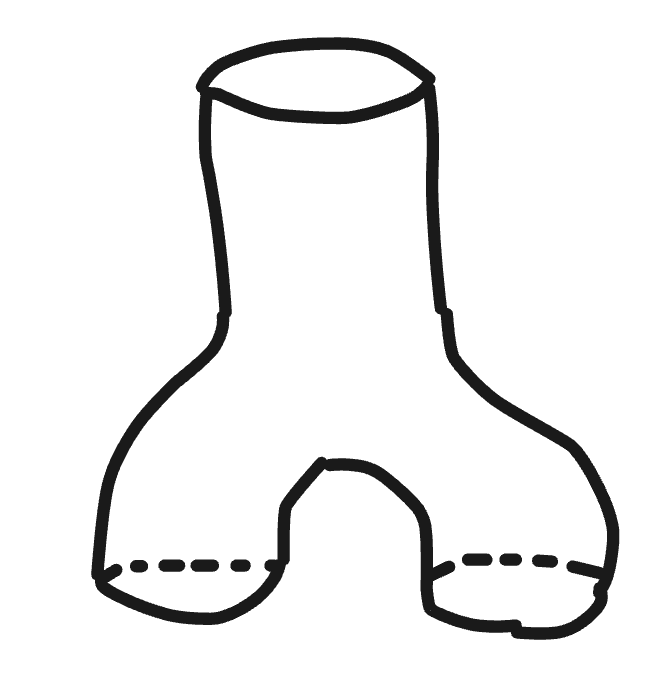
\includegraphics[scale=0.25]{mult.png}
  \end{center}
  and a binary co-operation $d : A \to A \otimes A$:
  \[
  A \xrightarrow{d} A \otimes A
  \]
  \begin{center}
  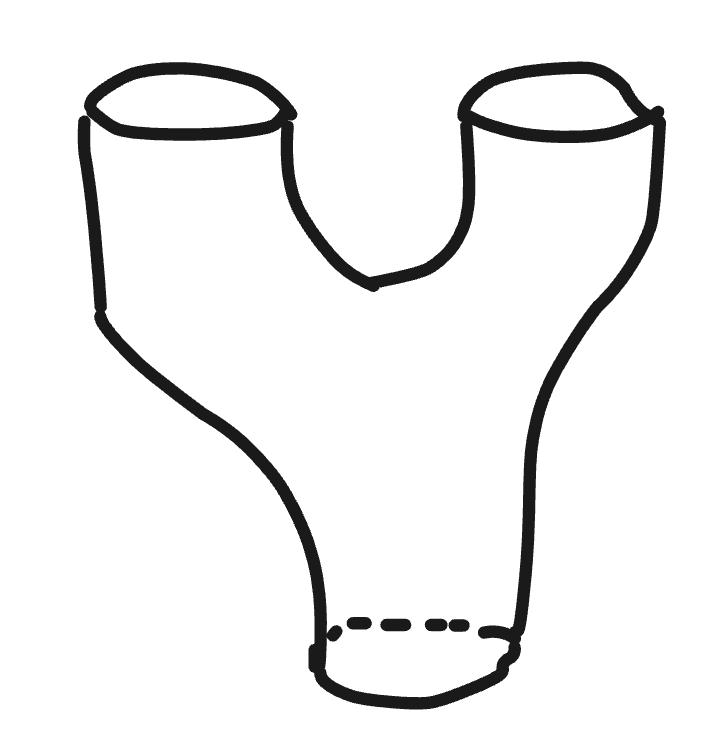
\includegraphics[scale=0.25]{comult.png}
  \end{center}
  such that they are associative and co-associative respectively, and $A$ is also equipped with
  a unit $e : I \to A$ and a counit $A \to I$:
  \begin{center}
  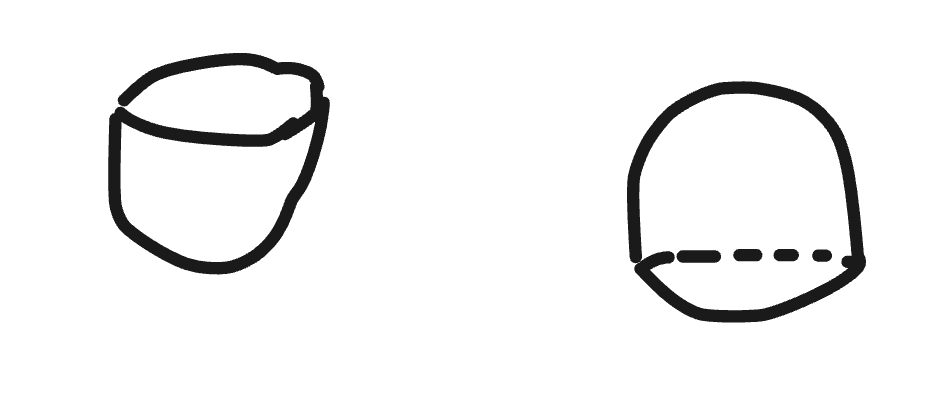
\includegraphics[scale=0.25]{unit-counit.png}
  \end{center}
  
  A bimonoid is \emph{Frobenius} is the following equalities are satisfied:
  \begin{center}
  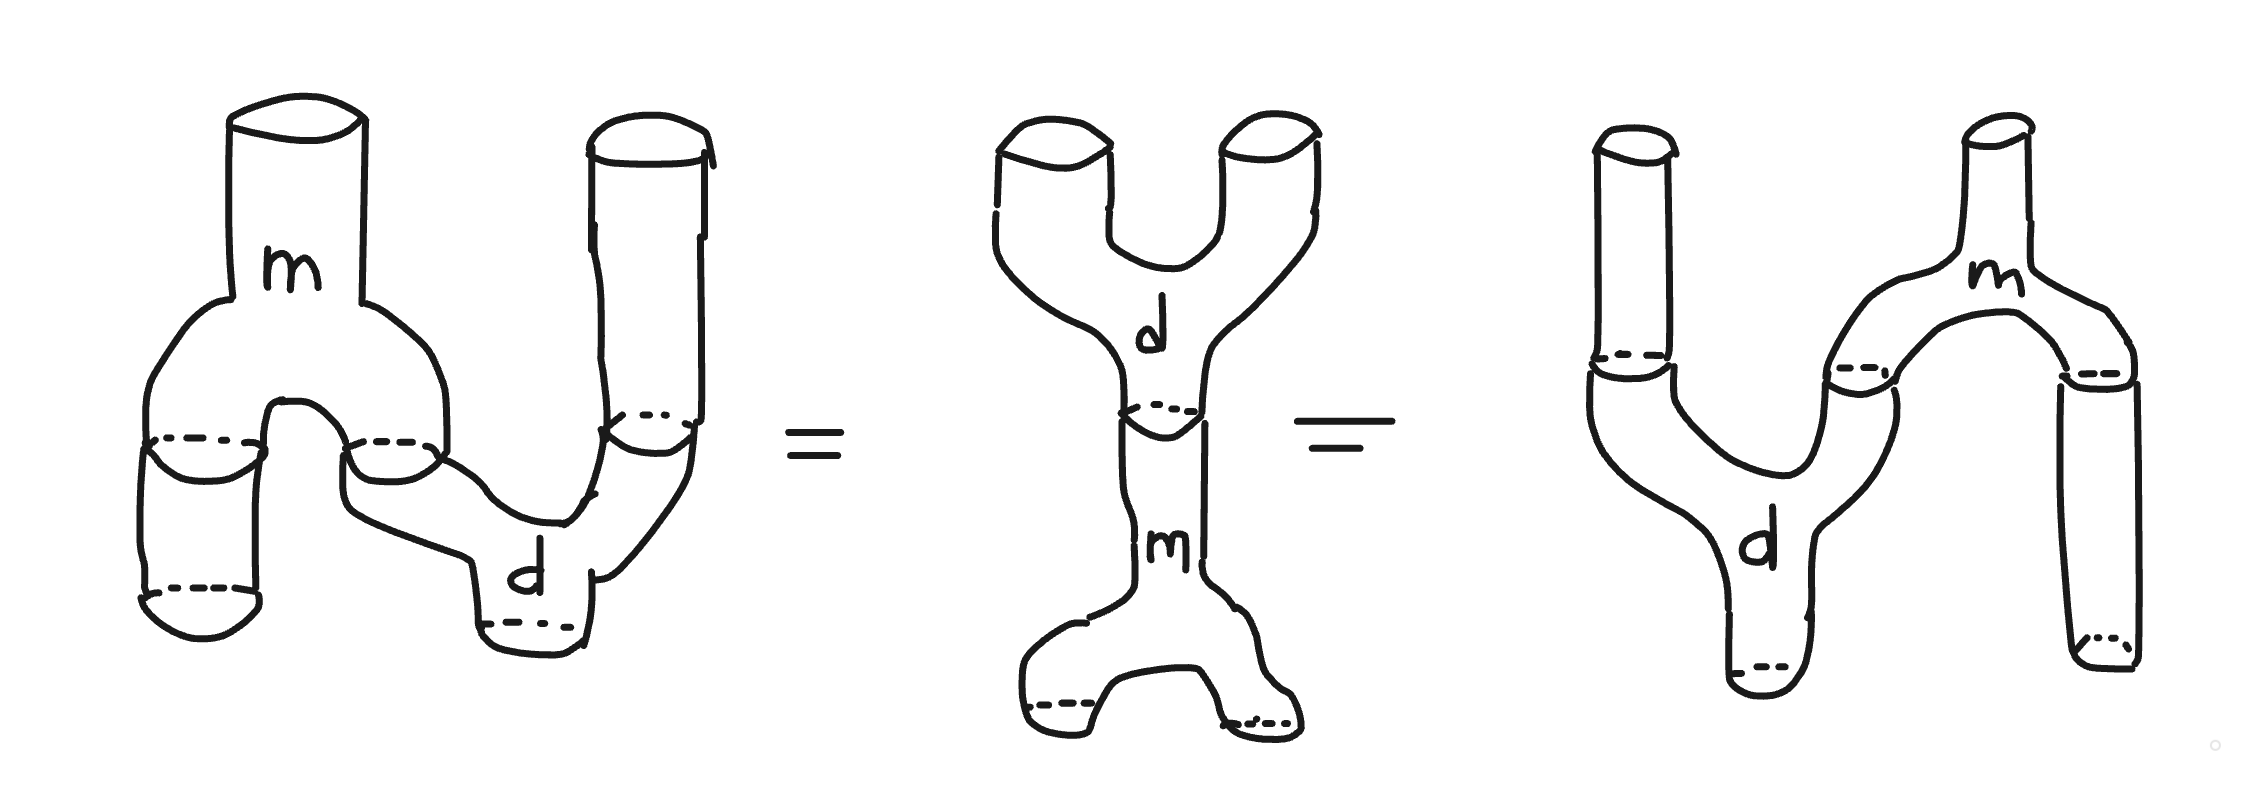
\includegraphics[scale=0.35]{frobenius-axiom.png}
  \end{center}

  A Frobenius monoid is commutative (cocommutative) if its monoid (comonoid) component is commutative (cocommutative).
\end{definition}

The characterisation of topological field theories of dimension 2 is generalisable to an arbitrary symmetric monoidal category.
\begin{prop}
  Let $\mathcal{V}$ be a symmetric monoidal category. 
  There is a 1-to-1 correspondence symmetric monoidal functor ${\bf Cob}(2) \to \mathcal{V}$
  and commutative and cocommutative Frobenius monoids.
\end{prop}

\begin{proof}
  See \cite{kock2004frobenius}.
\end{proof}

The further idea is to study Frobenius monoids in a more logical framework inspired by game semantics.
We decouple the monoid side $(A, m, e)$ from the comonoid side $(B, d, u)$ in the definition of
a Frobenius monoid. Different carriers describe the ``split personality'' aspect of the Frobenius monoid. We
differ operations from cooperations by the blue and red colours:
  \begin{center}
  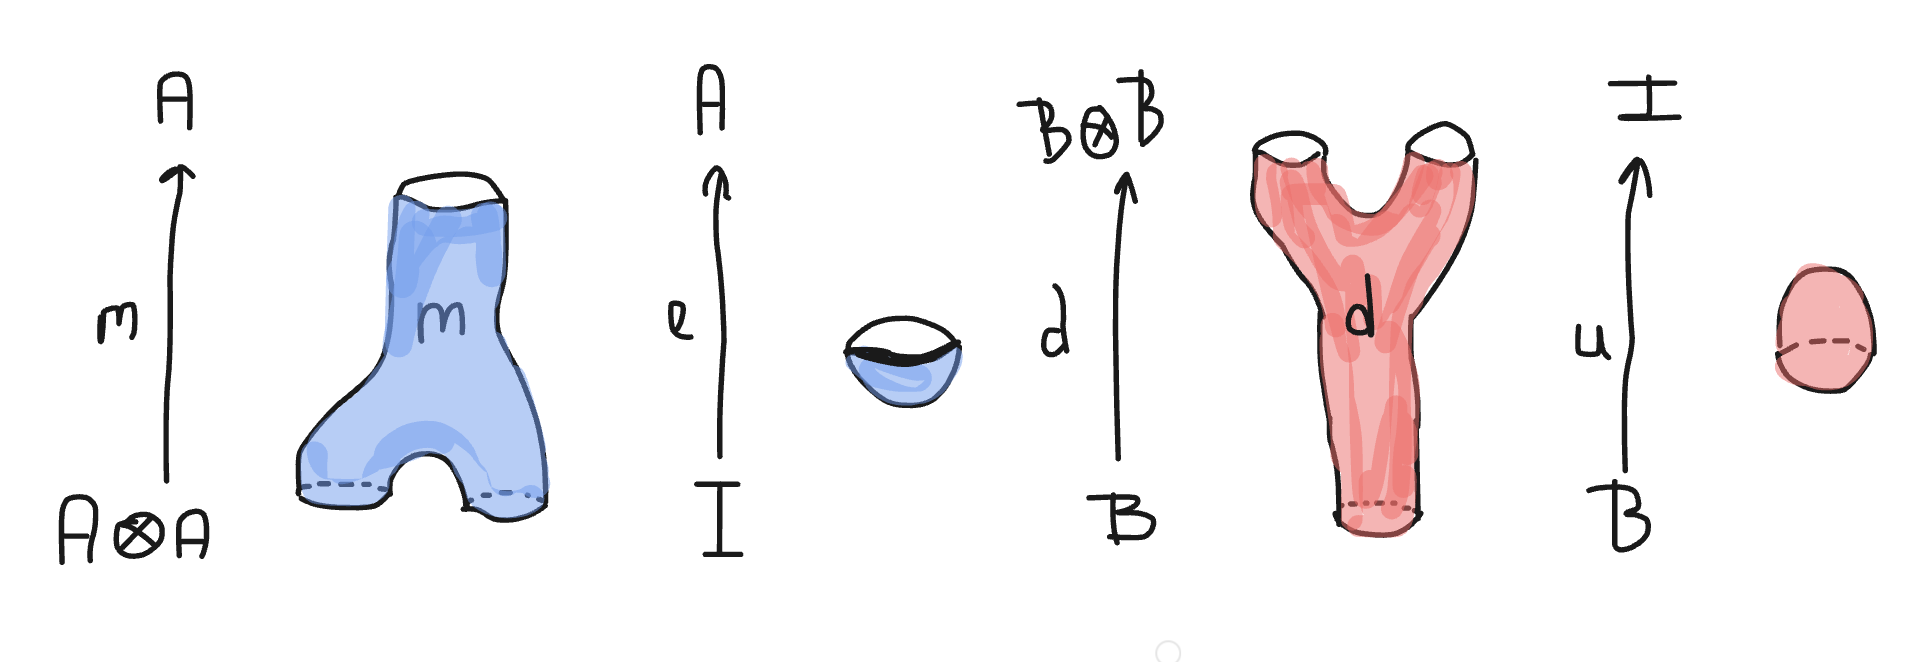
\includegraphics[scale=0.4]{blue-red-1.png}
  \end{center}

The question is how $A$ and $B$ are coupled inside a Frobenius monoid. First of all, $A$ and $B$ should be involved
in \emph{exact pairing} $A \dashv B$ defined as a pair of morphisms:
\begin{itemize}
  \item $\eta : I \to B \otimes A$
  \item $\varepsilon : A \otimes B \to I$
\end{itemize}
satisfying the following zig-zag equations:
  \begin{center}
  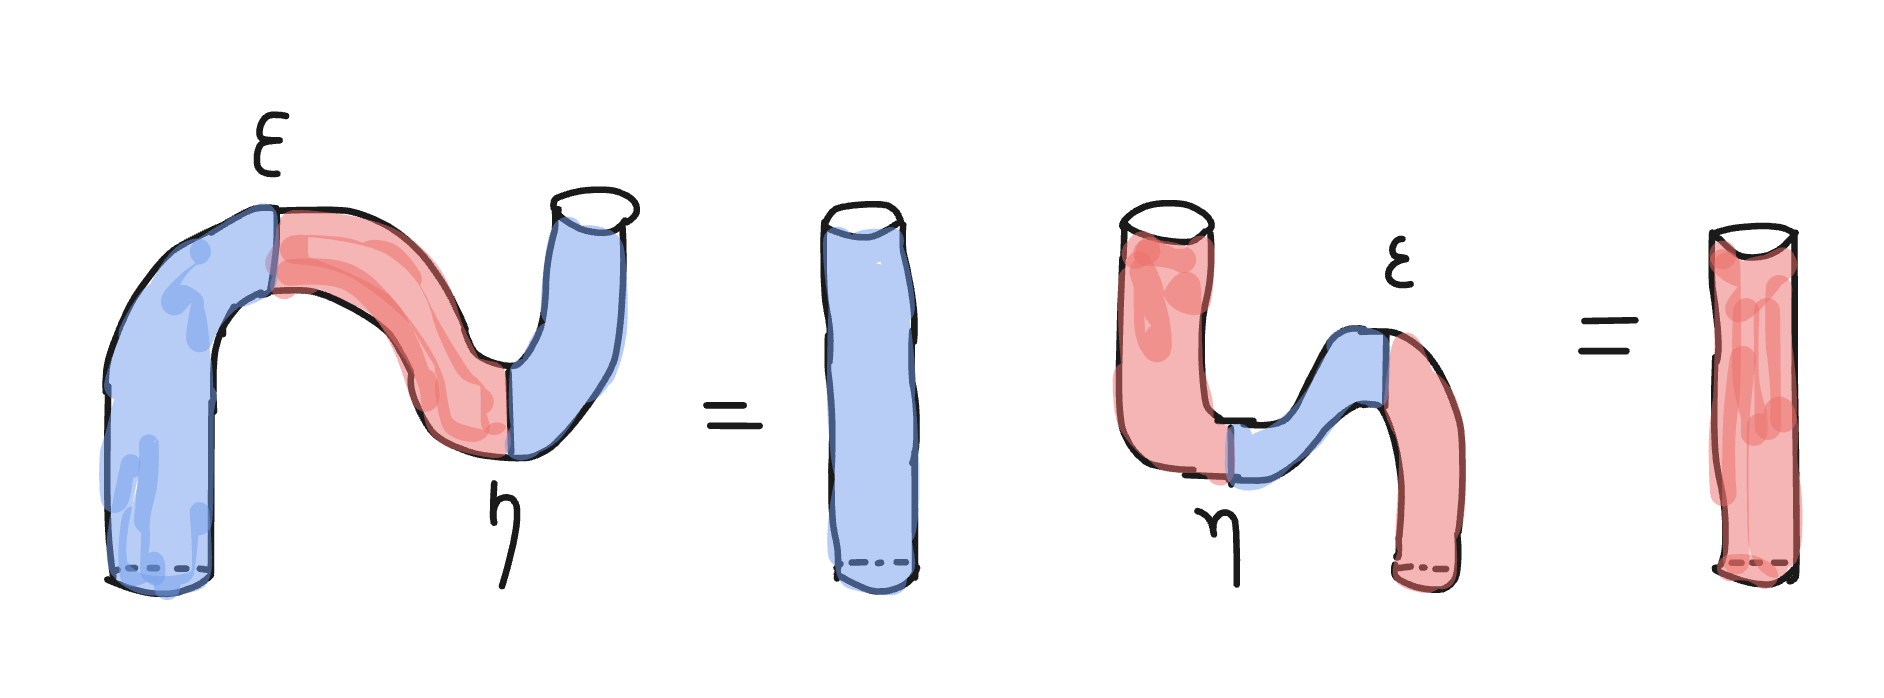
\includegraphics[scale=0.4]{blue-red-2.png}
  \end{center}

If $\mathcal{V}$ is the category of $k$-vector spaces, one can equip $A$ and $B$ with a non-degenerate
form $\varepsilon : A \otimes B \to k$. The exact pairing $A \dashv B$ should be compatible
with the comonoid and monoid structures the following way. We define a monoid-comonoid pairing:
\[
(A, m, e) \dashv (B, d, u)
\]
between a monoid and a comonoid as an exact pairing between carriers $A \dashv B$ satisfying the following two equalities:
  \begin{center}
  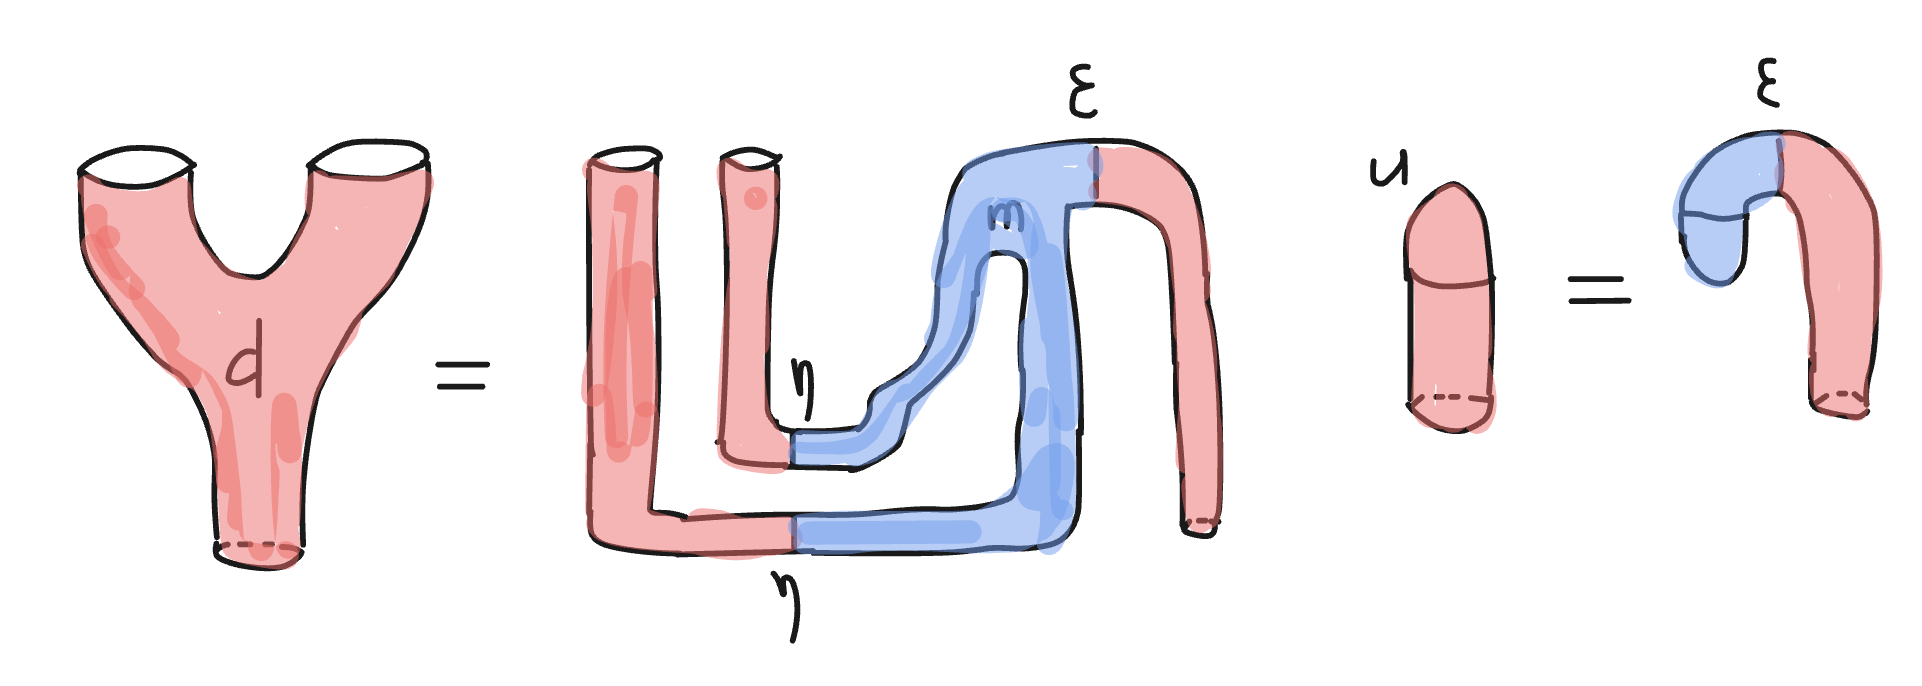
\includegraphics[scale=0.4]{blue-red-3.png}
  \end{center}

Those equations mean that the comonoid structure $(B, d, u)$ can be recovered from the monoid structure
$(A, m, e)$ on $A$ and the other way round. Symmetrically, the existence of a monoid-comonoid pairing
\[
(B, d, u) \dashv (A, m, e)
\]
defined as an exact pairing $B \dashv A$ between the underlying objects with the components
\begin{itemize}
  \item $\eta' : I \to B \otimes A$
  \item $\varepsilon' : A \otimes B \to I$
\end{itemize}
satisfying the following equations:
  \begin{center}
  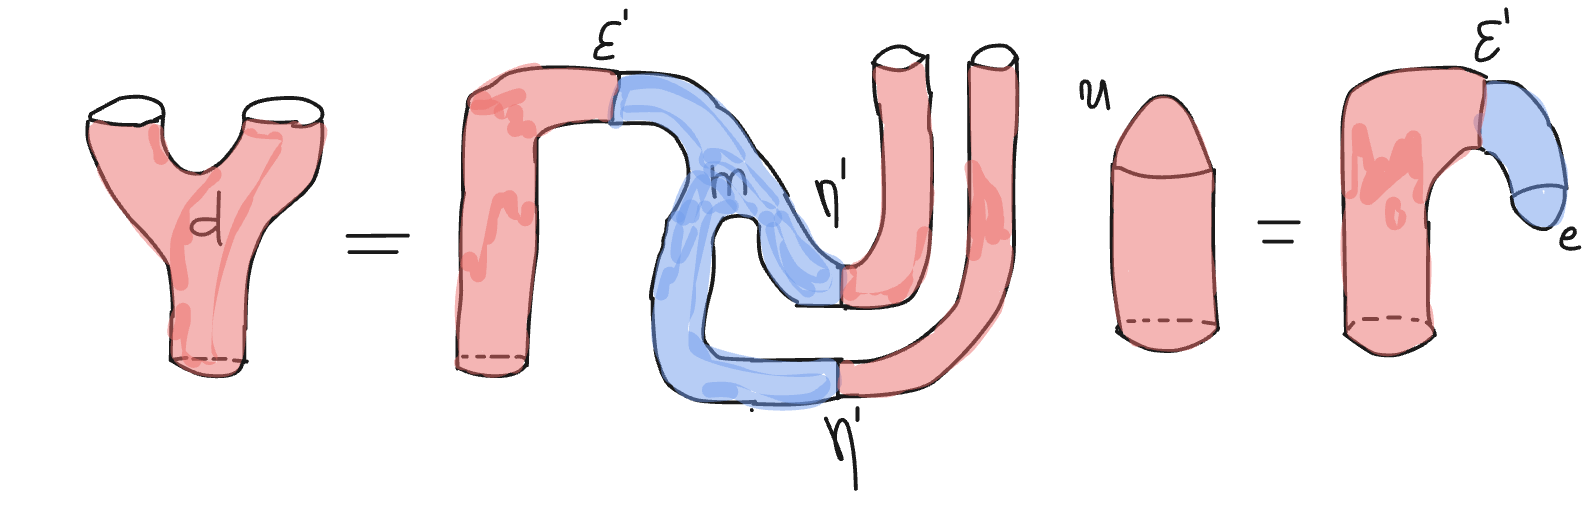
\includegraphics[scale=0.5]{blue-red-4.png}
  \end{center}

This leads to the definition of a Frobenius pair:
\begin{definition}
  A Frobenius pair in a symmetric monoidal category $\mathcal{V}$ consists of a monoid-comonoid exact pairing:
  \[
  (A, m, e) \dashv (B, d, u)
  \]
  and a comonoid-monoid pairing
  \[
  (B, d, u) \dashv (A, m, e)
  \]
  along with an isomorphism $L : A \cong B$ such that the following is satisfied:
  \begin{center}
  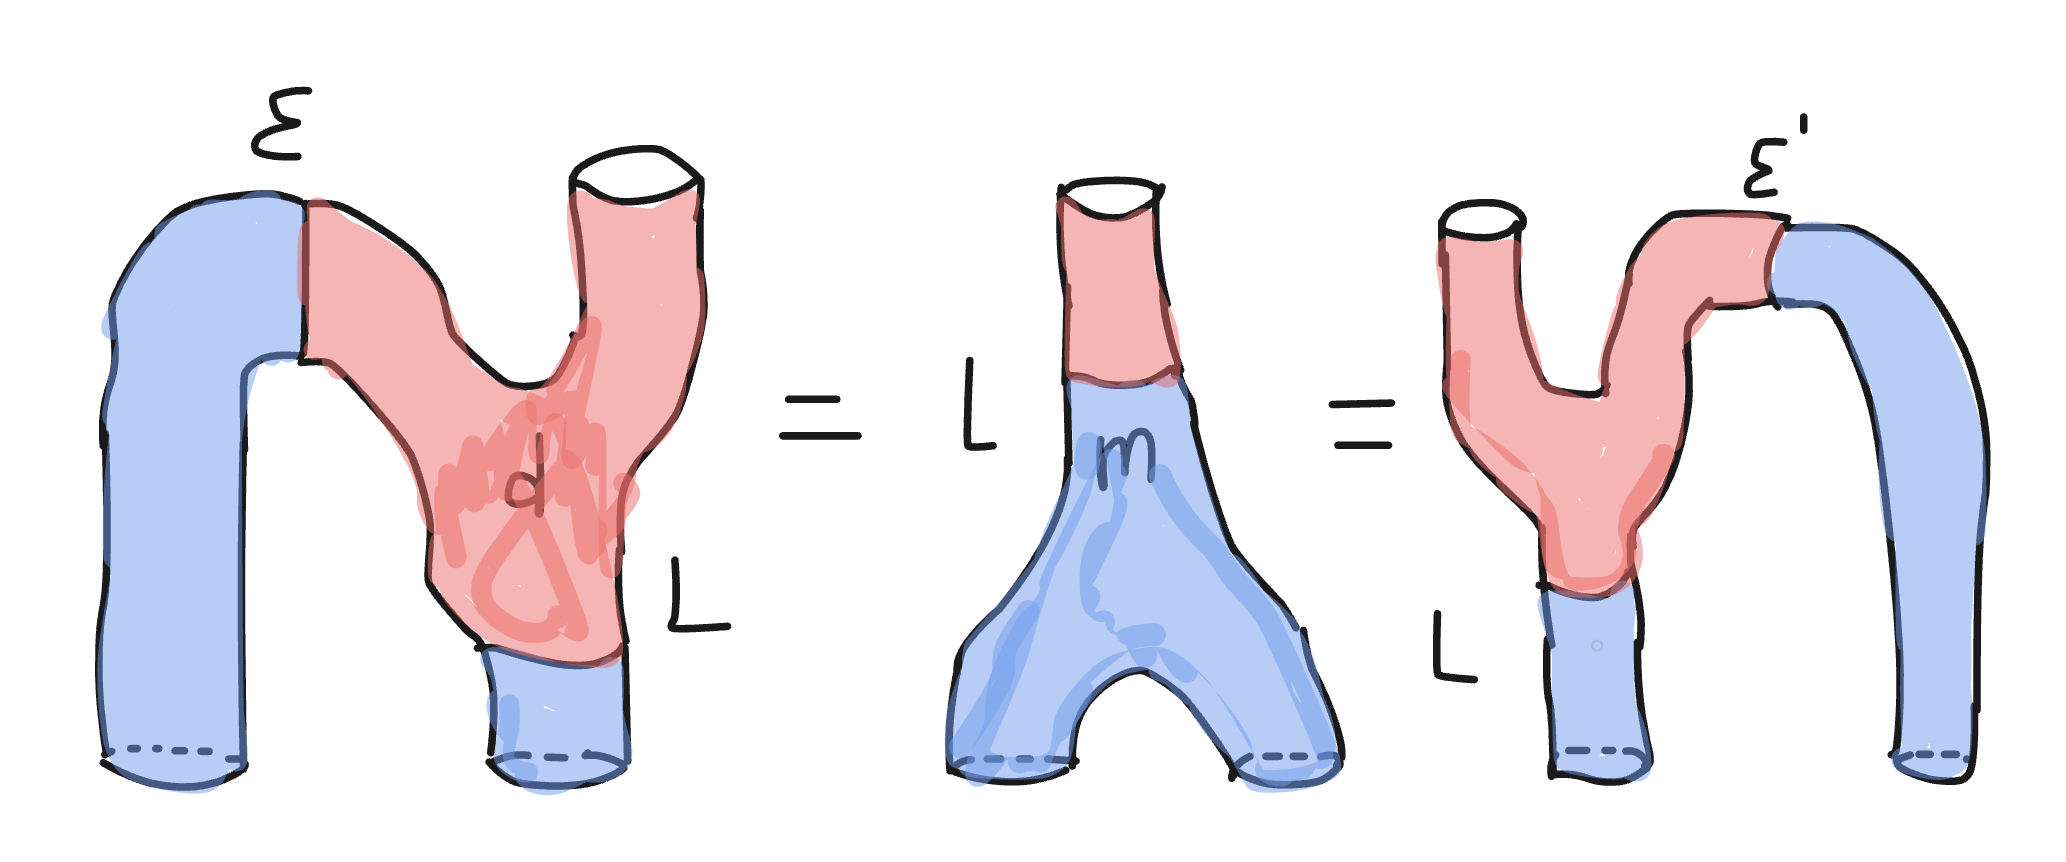
\includegraphics[scale=0.35]{blue-red-5.png}
  \end{center}
\end{definition}
The above equations have the following reformulation:
   \begin{center}
  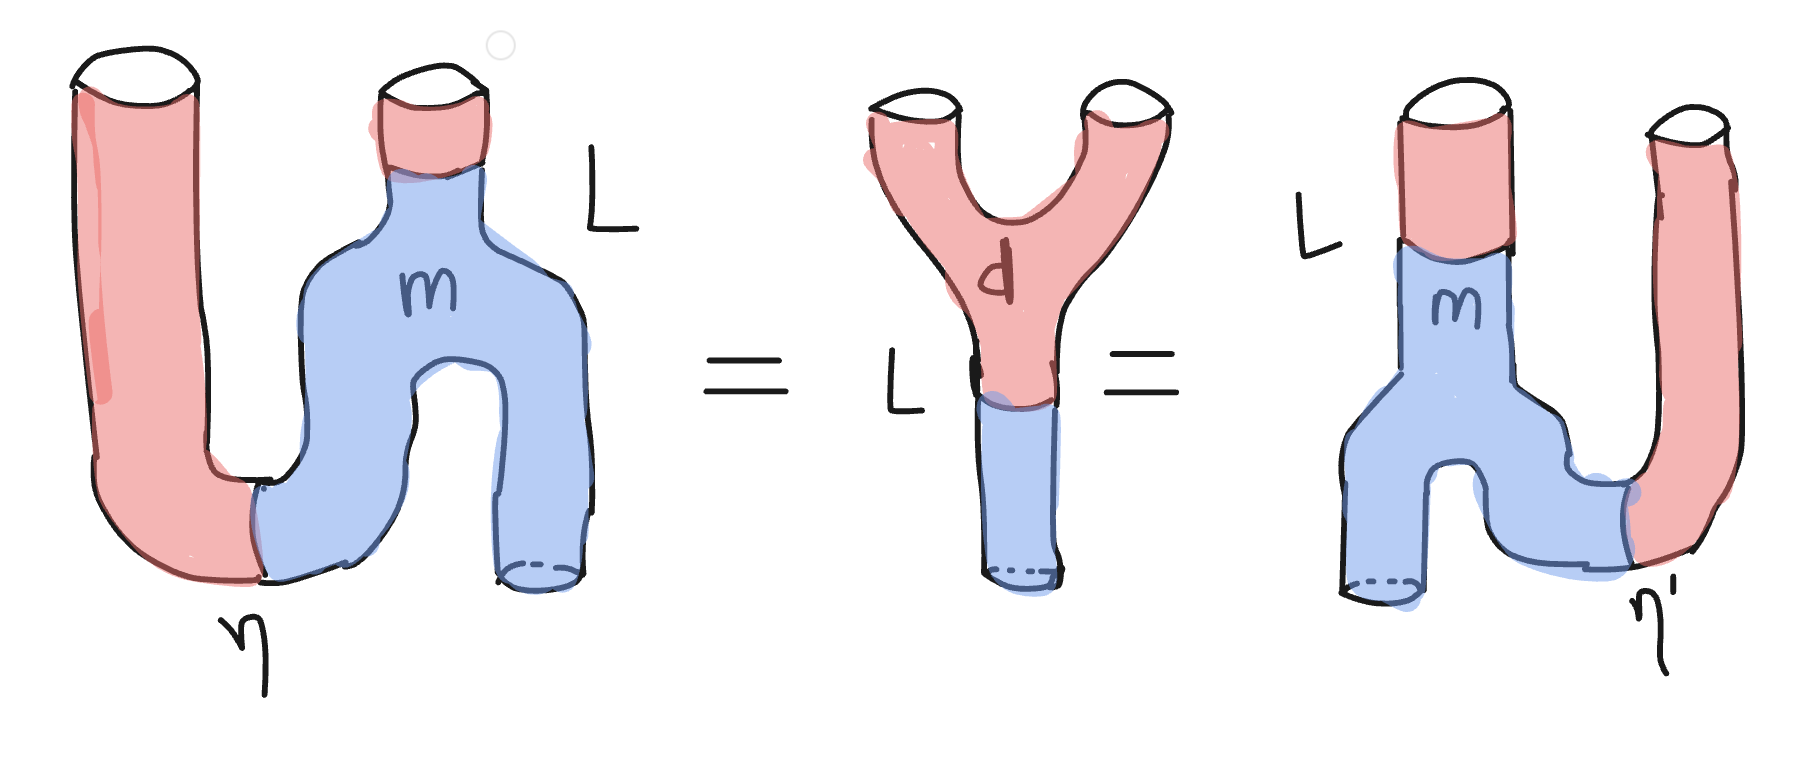
\includegraphics[scale=0.45]{blue-red-6.png}
  \end{center}

These equalities have the following interpretation. The monoid-comonoid pairing $(A, m, e) \dashv (B, d, u)$
induces a left action of the monoid $(A, m, e)$ on $B$:
  \begin{center}
  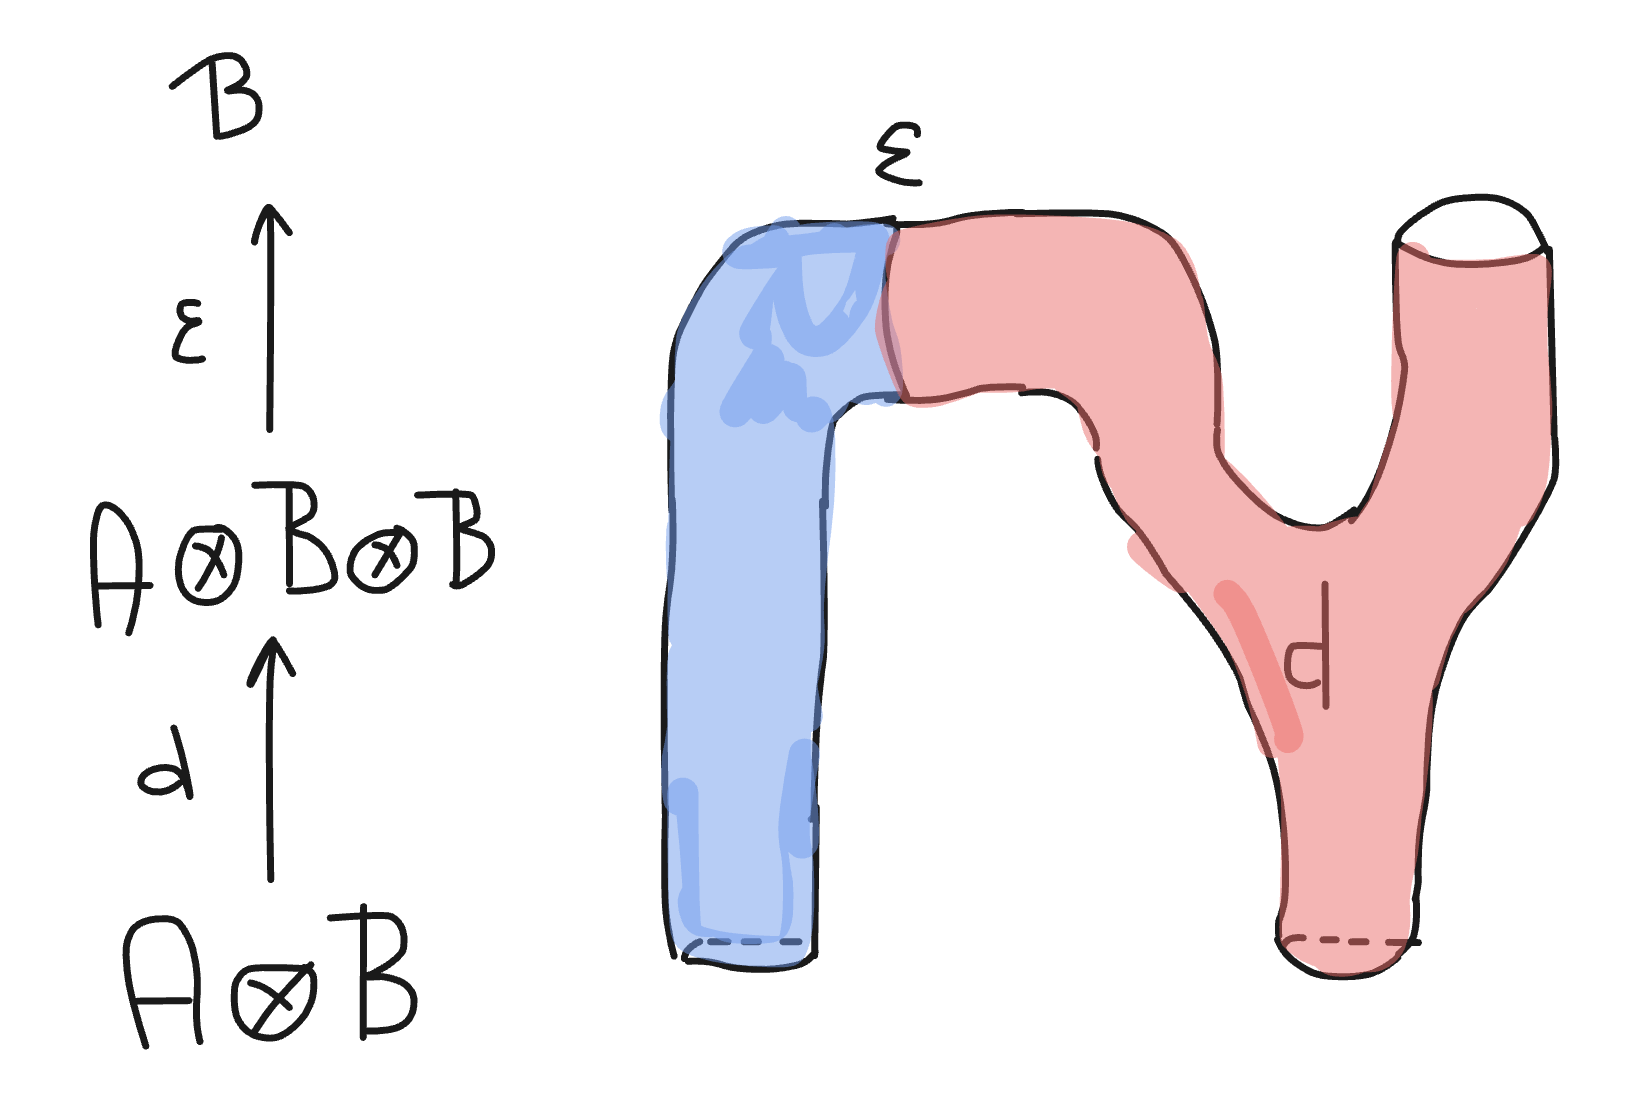
\includegraphics[scale=0.25]{blue-red-7.png}
  \end{center}

The equation from the definition of a Frobenius pair means that the morphism $L$ transports 
the left action of the monoid $A$ on itself into the action of $A$ on the comonoid carrier $B$. Symmetrically,
the exact pairing $B \dashv A$ a right action of the monoid $A$ on $B$, so the second equation from the definition
of a Frobenius pair asks that $L$ transports the canonical right action of $A$ on itself into the right
action of $A$ on $B$. There is the following correspondence between Frobenius pairs and Frobenius monoids.

\begin{prop} Let $\mathcal{V}$ be a monoidal category, then
  there is a 1-to-1 correspondence between Frobenius pairs $(A, B)$ and Frobenius monoids $A$ 
  equipped with an exact pairing $A \dashv B$.
\end{prop}

\begin{proof}
  Given a Frobenius monoid $A$ with an exact pairing $A \dashv B$ and unit $\eta$ and counit $\varepsilon$,
  then one defines the unit $\eta'$ and the counit $\varepsilon'$ of the exact pairing $B \dashv A$ and the isomorphism $L$
  the following way:
  \begin{center}
  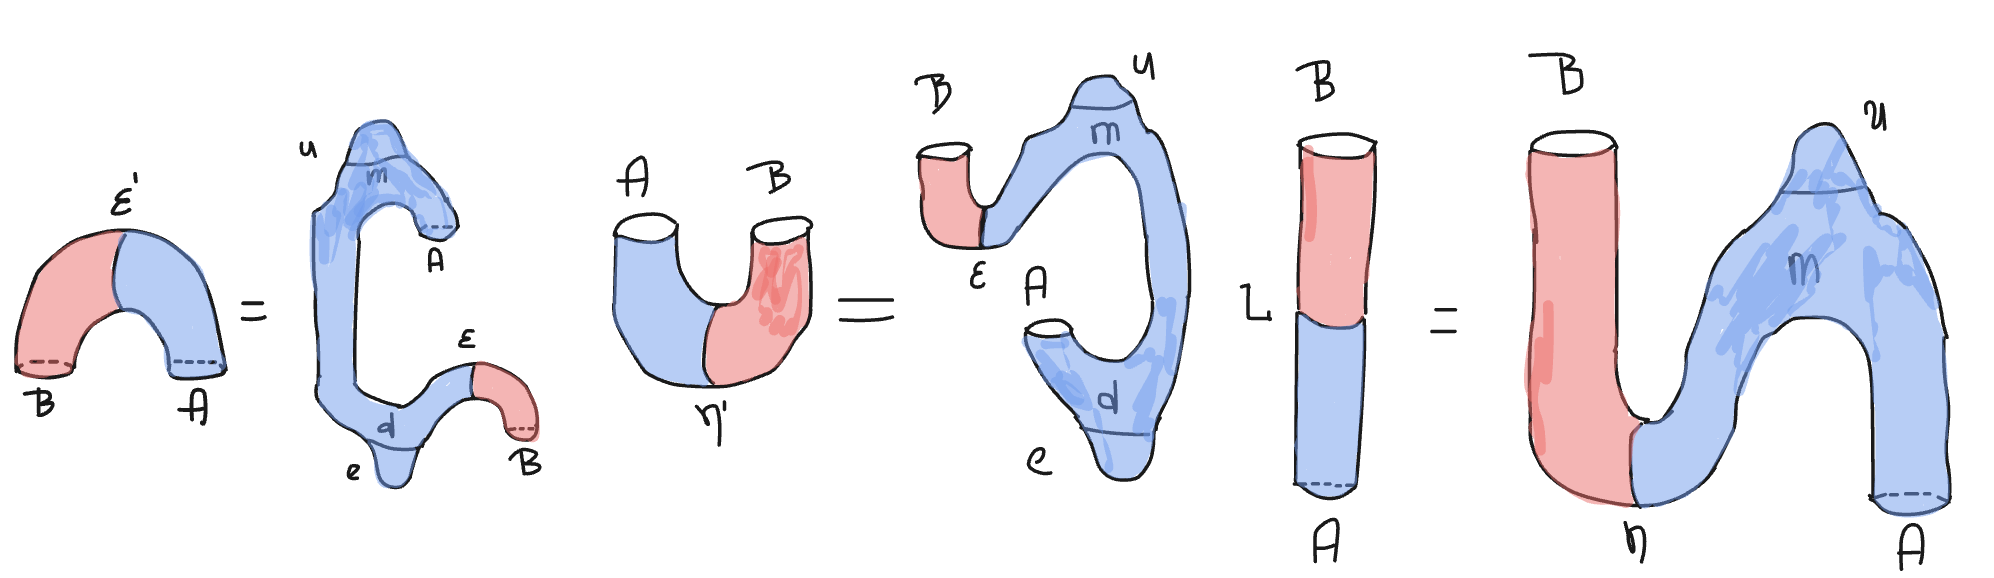
\includegraphics[scale=0.45]{blue-red-8.png}
  \end{center}

  $B$ inherits the comonoid structure $(B, d, u)$ from the monoid structure $(A, m, e)$ and the exact pairing
  $A \dashv B$. Then one checks that the comonoid structure coincides with the comonoid structure induced by
  the exact pairing $B \dashv A$. Finally, one checks the equalities the equalities from the definition of a Frobenius pair.
  Conversely, any Frobenius pair $(A, B)$ induces a Frobenius monoid on $A$ with the monoid structure 
  $(A, m, e)$ and the comonoid structure $(A, d', u')$ induced with the isomorphism with $(B, d, u)$ by $L$.
\end{proof}

Let $(A, B)$ be a Frobenius pair in a monoidal category $\mathcal{V}$, the following morphism
  \begin{center}
  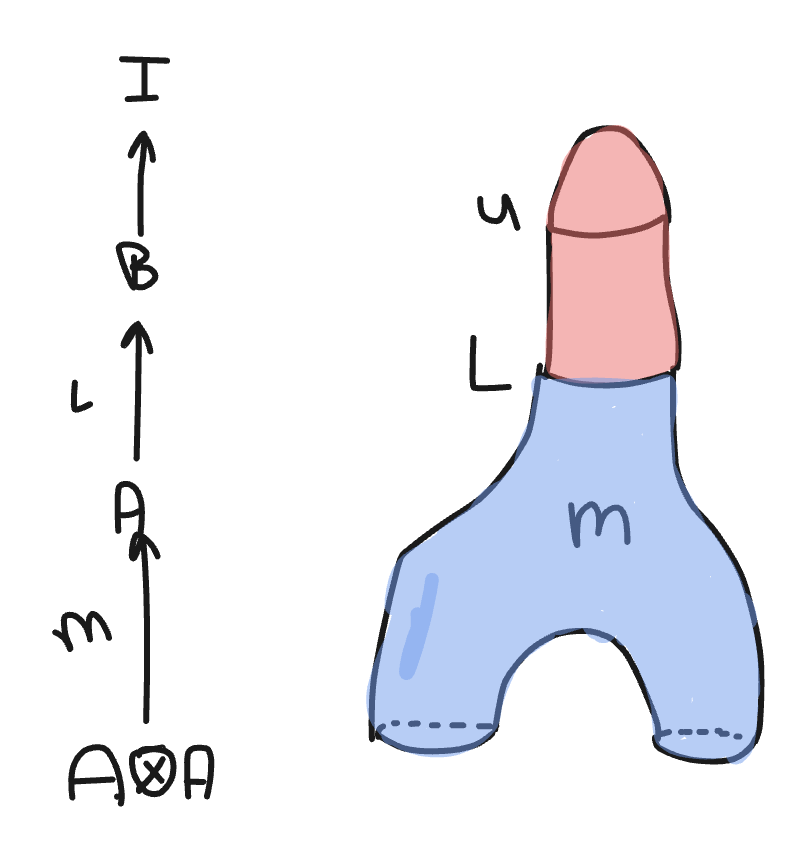
\includegraphics[scale=0.35]{blue-red-9.png}
  \end{center}
defined a bilinear form $||.,.|| : A \otimes A \to I$ called the \emph{Frobenius bracket}. The definition of 
a Frobenius bracket ensures that the following condition is satisfied:
\[
||a_1 \bullet a_2, a_3|| = || a_1, a_2 \bullet a_3 ||
\]
Using the definition of a Frobenius pair, one can reformulate the definition of a Frobenius brackets the following way:
  \begin{center}
  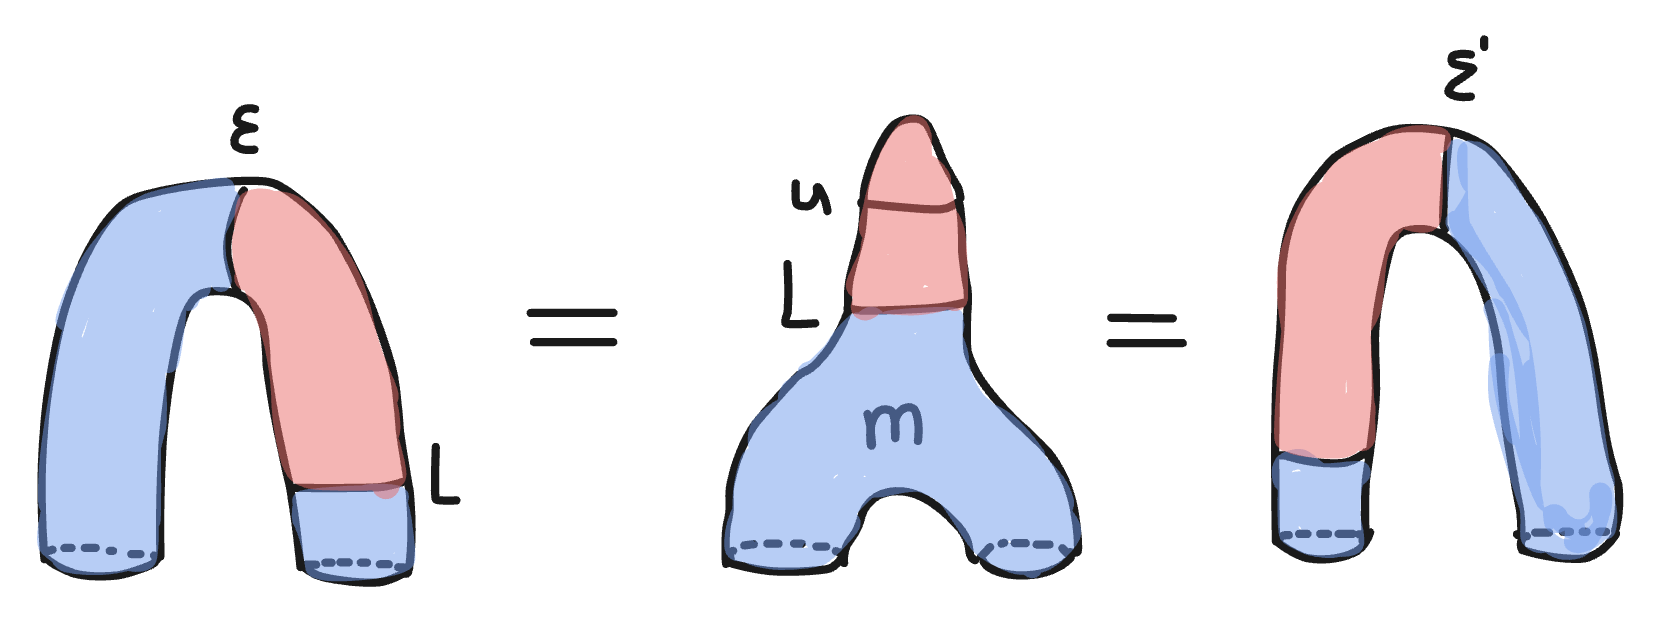
\includegraphics[scale=0.35]{blue-red-10.png}
  \end{center}

A \emph{braiding} for a monoidal category $\mathcal{V}$ is a family of natural isomorphisms:
\[
\gamma_{A, B} : A \otimes B \to B \otimes A
\]
such that the following diagrams commute:
\[
\begin{tikzcd}
  & A \otimes (B \otimes C) \ar[rr, "\gamma_{A, B \otimes C}"] && (B \otimes C) \otimes A \ar[dr, "a_{B,C,A}"] \\
  (A \otimes B) \otimes C \ar[ur, "a_{A,B,C}"] \ar[dr, "\gamma_{A,B} \otimes 1_C"'] &&&& B \otimes (C \otimes A) \\
  & (B \otimes A) \otimes C \ar[rr, "a_{B,A,C}"'] && B \otimes (A \otimes C) \ar[ur, "\gamma_{A,C} \otimes 1"']
\end{tikzcd}
\]
\[
\begin{tikzcd}
  & (A \otimes B) \otimes C \ar[rr, "\gamma_{A \otimes B, C}"] && C \otimes (A \otimes B) \ar[dr, "a{-1}_{C,A,B}"] \\
  A \otimes (B \otimes C) \ar[ur, "a^{-1}_{A,B,C}"] \ar[dr, "1 \otimes \gamma_{B,C}"'] &&&& (C \otimes A) \otimes B \\
  & A \otimes (C \otimes B) \ar[rr, "a^{-1}_{A,C,B}"] && (A \otimes C) \otimes B \ar[ur, "\gamma_{A,C} \otimes 1"']
\end{tikzcd}
\]

A \emph{braided monoidal category} is a monoidal category with a choice of braiding.


Let $\mathcal{V}$ be a braided monoidal category, a twist for $\mathcal{V}$ is a family of isomorphisms $\theta_A : A \to A$
such that $\theta_I = 1_I$ and
\[
\begin{tikzcd}
  A \otimes B \ar[r, "\gamma_{A,B}"] \ar[d, "\theta_{A \otimes B}"'] & B \otimes A \ar[d, "\theta_B \otimes \theta_A"] \\
  A \otimes B & B \otimes A \ar[l, "\gamma_{B,A}"]
\end{tikzcd}
\]

A \emph{balanced monoidal category} is a braided monoidal category with a choice of a twist. 

Typically, a balanced monoidal category $\mathcal{V}$ is given as $\mathcal{V} = {\bf Mod}(H)$, the category of representations
of a quantum group $H$. The braiding $\gamma$ and the twist $\theta$ are represented as follows:
  \begin{center}
  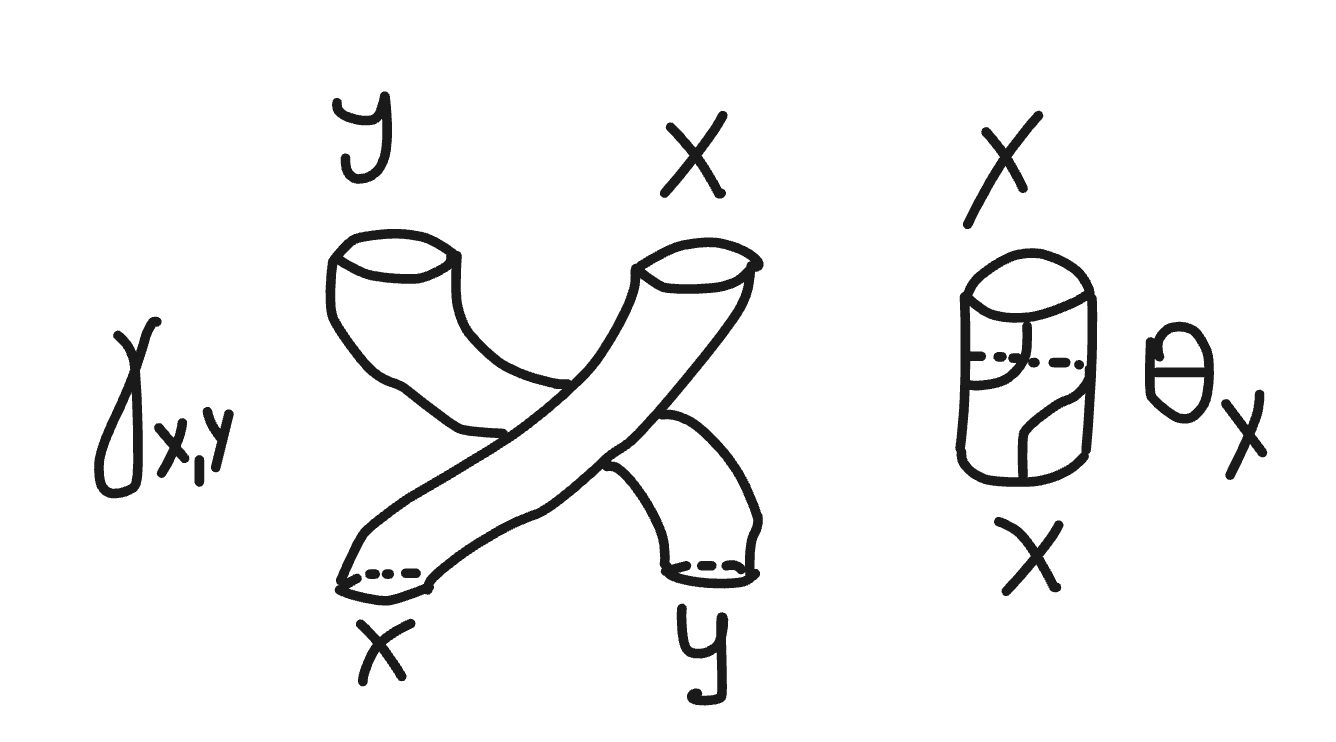
\includegraphics[scale=0.28]{braid-and-twist.png}
  \end{center}

The twist $\theta_X$ is understood as the operation of applying a rotation of angle $2 \pi$ on the border
$X$ of the two-dimensional manifold. The extra structure allows formulating the definition of helical Frobenius monoid.

\begin{definition}
  A Frobenius monoid $A$ in a balanced monoidal category $\mathcal{V}$ is called \emph{helical} if the following is satisfied:
  \begin{center}
  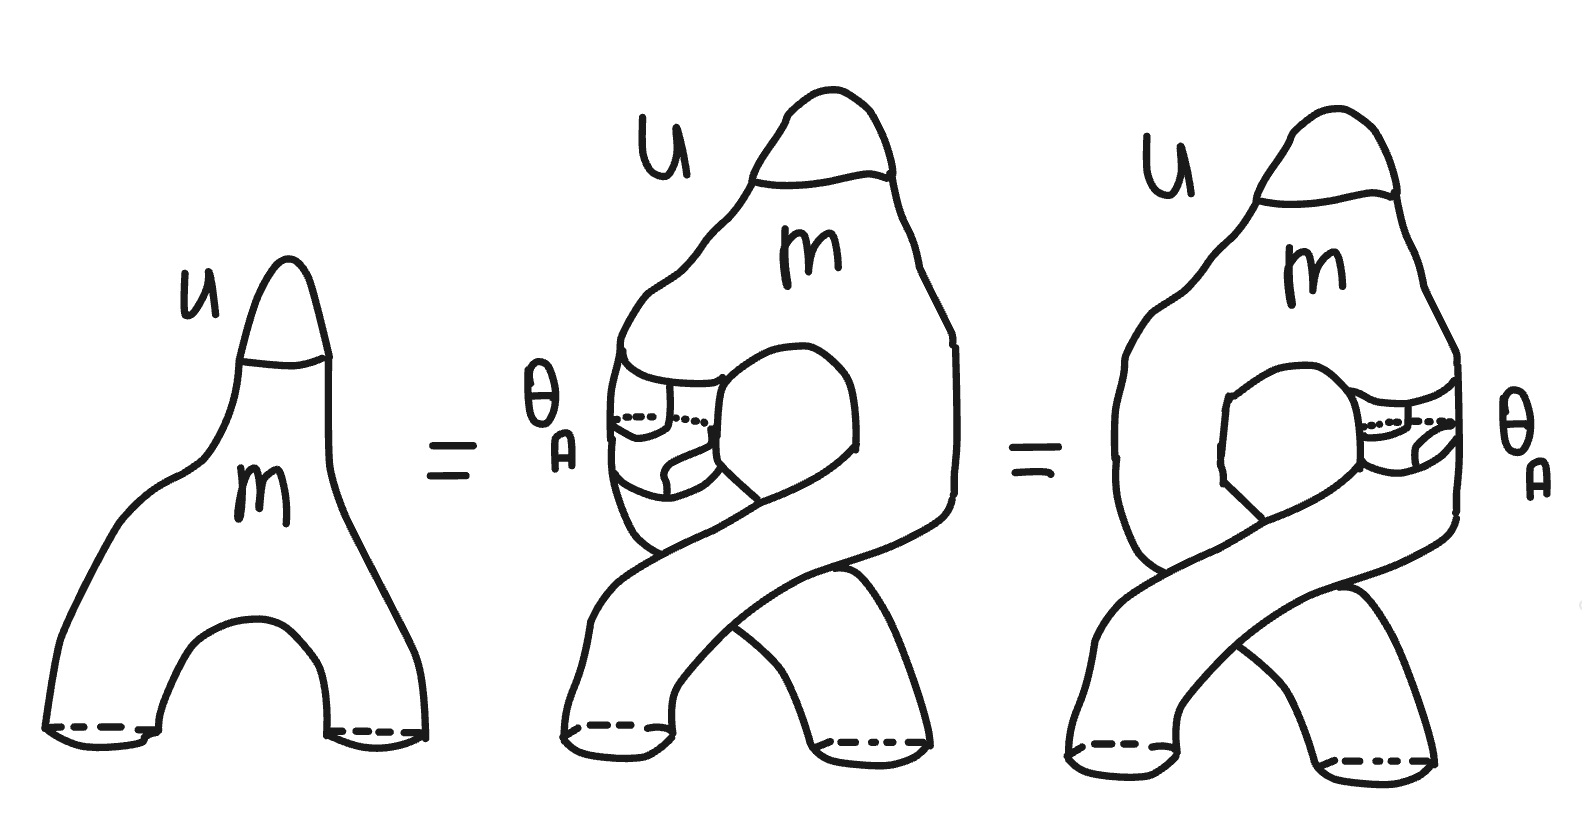
\includegraphics[scale=0.28]{helical-frobenius.png}
  \end{center}
\end{definition}

\begin{definition}
  A Frobenius pair $(A, B)$ is a balanced monoidal category is \emph{helical} if the following equalities are satisfied:
    \begin{center}
  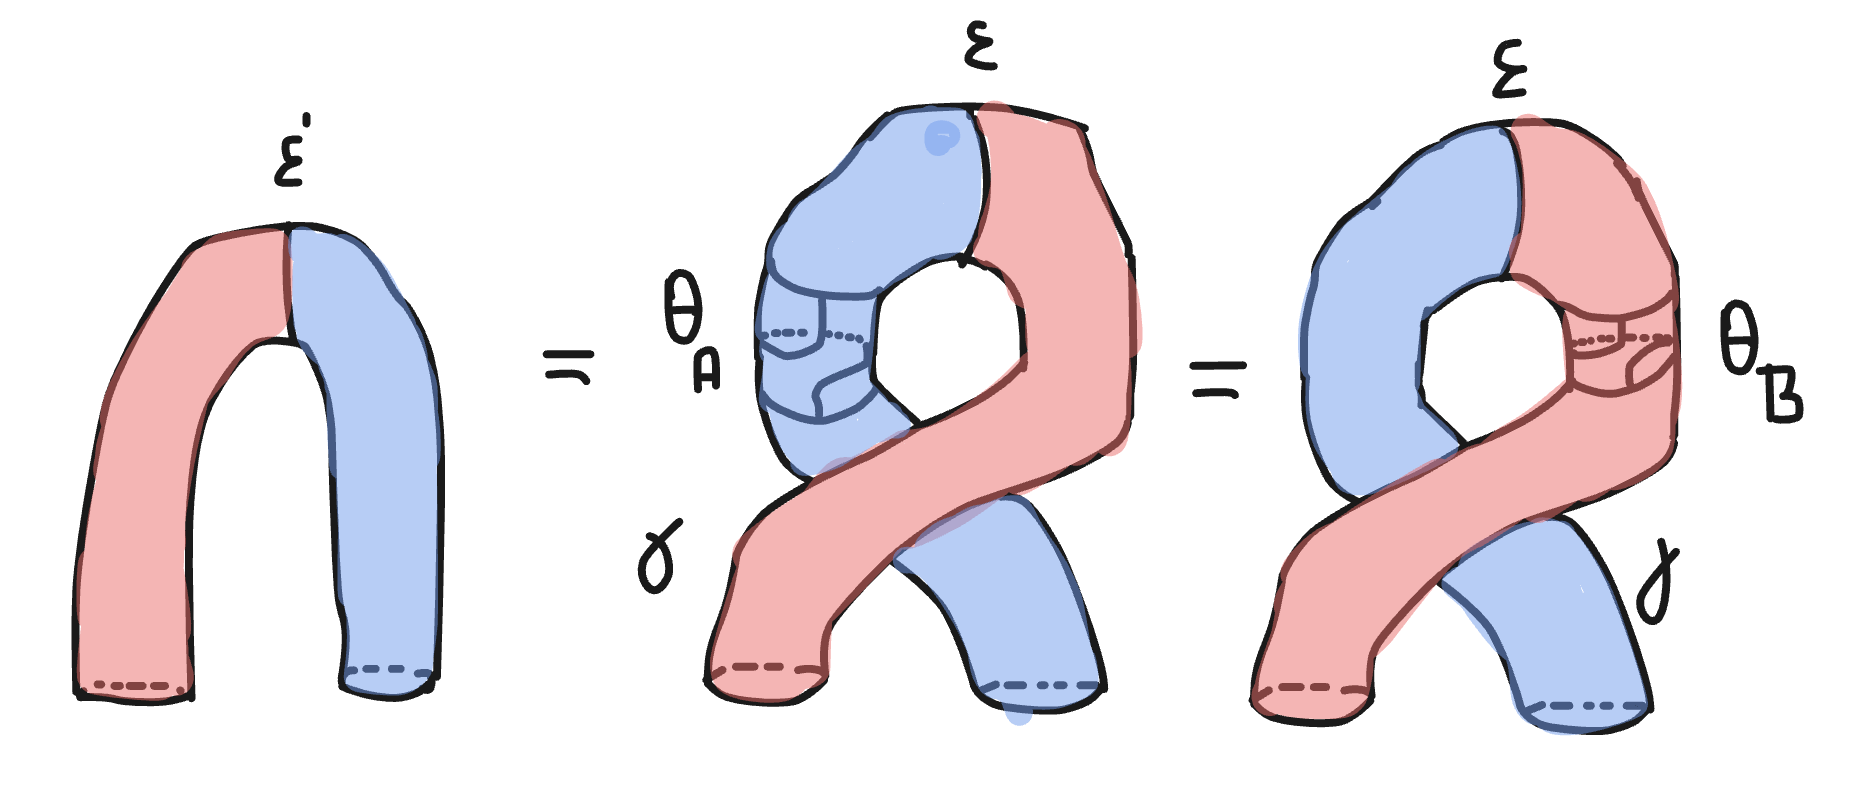
\includegraphics[scale=0.33]{blue-red-11.png}
  \end{center}
\end{definition}

One can reword the definition of helicality of a Frobenius pair the following way using the reversibility of $L$:
  \begin{center}
  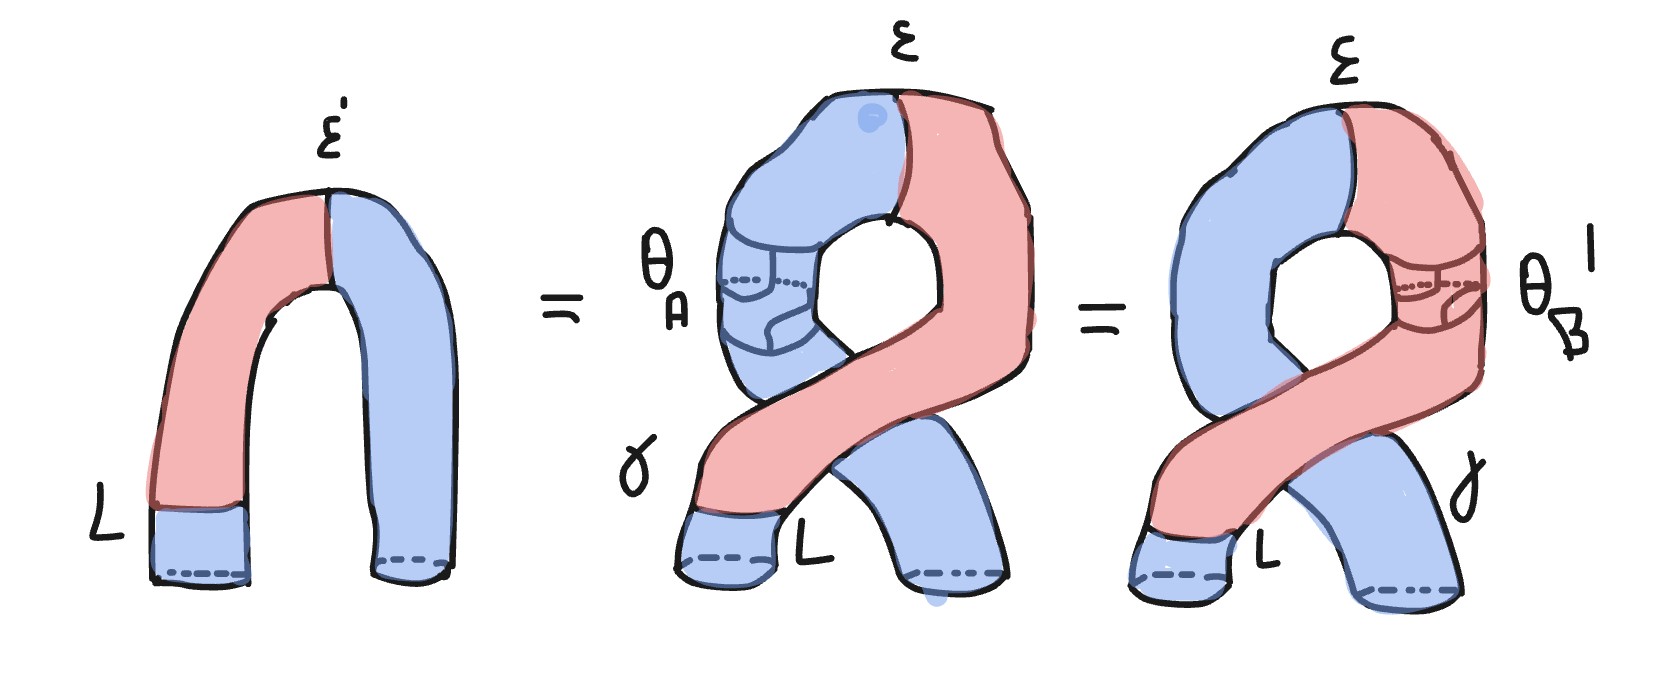
\includegraphics[scale=0.36]{blue-red-12.png}
  \end{center}

In turn, the above condition is equivalent to the condition claiming that the Frobenius bracket is commutative in the sense of the following equalities:
  \begin{center}
  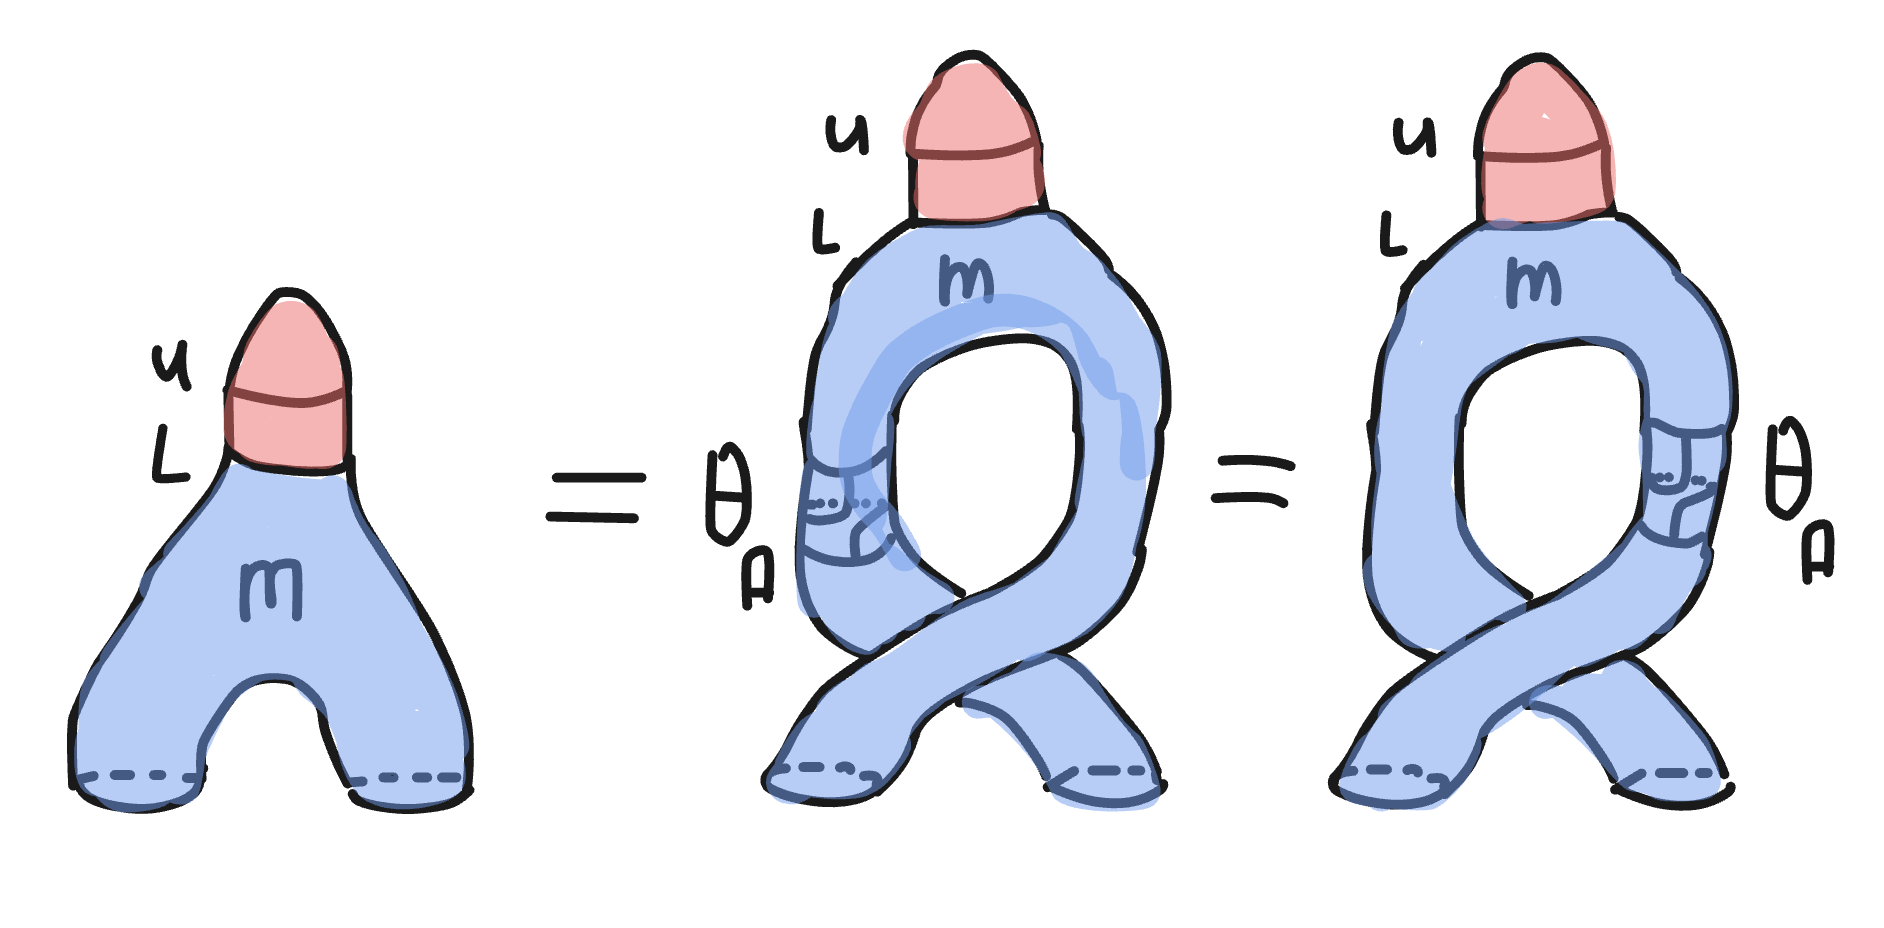
\includegraphics[scale=0.33]{blue-red-13.png}
  \end{center}

The above equivalence, in turn, follows from the fact that the twist operation is a natural isomorphism of the identity functor
with itself, and, therefore, the following is satisfied:
  \begin{center}
  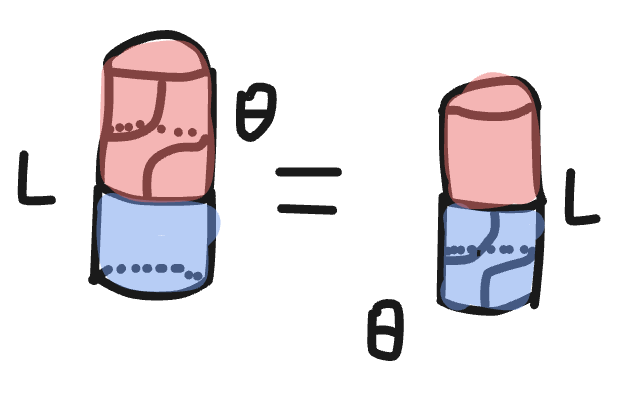
\includegraphics[scale=0.33]{blue-red-14.png}
  \end{center}

So we rephrase the condition the following algebraic way:
\[
||a_1, a_2 || = ||a_2, a_1||
\]
Thus we have the following cycling property of the Frobenius bracket:
\[
|| a_1 \bullet a_2, a_3 || = || a_3 \bullet a_1, a_2 || = ||a_2 \bullet a_3, a_1 ||.
\]

\begin{prop}
  Let $\mathcal{V}$ be a balanced monoidal category, then there is a 1-to-1 correspondence between helical Frobenius pairs and helical Frobenius monoids $A$
  equipped with exact pairing $A \dashv B$.
\end{prop}

\begin{definition}
  Let $\mathcal{V}$ be a balanced monoidal category, then $\mathcal{V}$ is \emph{ribbon} if each $A \in \mathcal{V}$
  is equipped with an exact pairing $A \dashv A^*$ whose counit $\varepsilon_A : A \otimes A^* \to I$ satisfies the following equatition:
  \begin{center}
  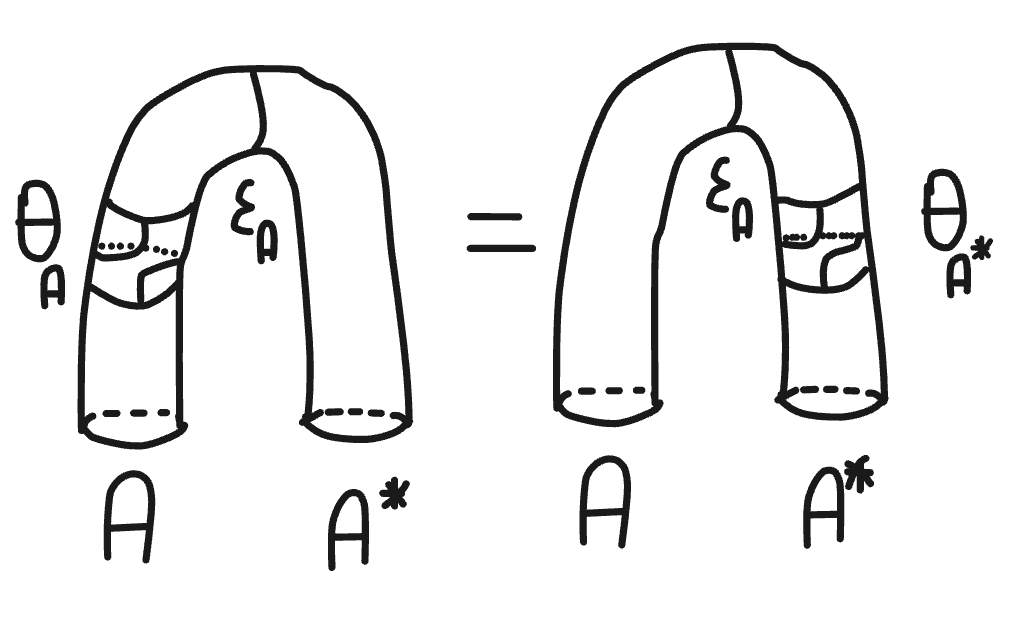
\includegraphics[scale=0.3]{ribbon.png}
  \end{center}
\end{definition}

From this definition, we have that if the right dual $A^*$ of $A$ is also a left dual of $A$, when counit $\varepsilon'_A$ of the exact
pairing $A^* \dashv A$ defined the following way:
  \begin{center}
  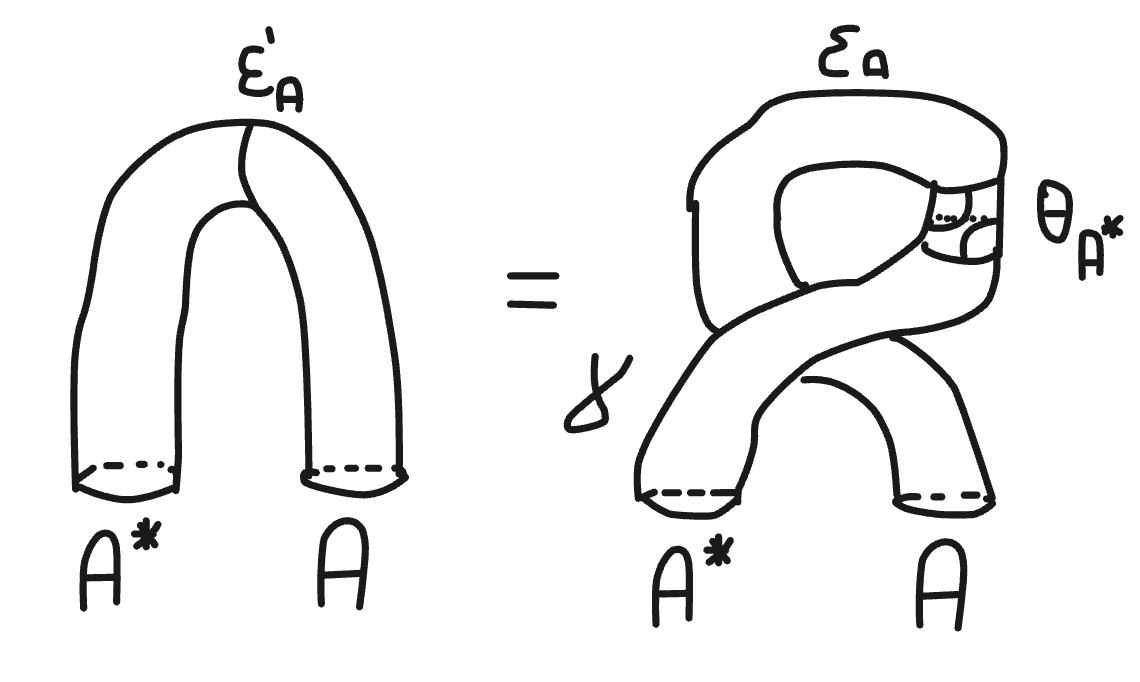
\includegraphics[scale=0.3]{ribbon-2.png}
  \end{center}

Also, any Frobenius pair in a ribbon category $\mathcal{V}$ satisfies the following:
  \begin{center}
  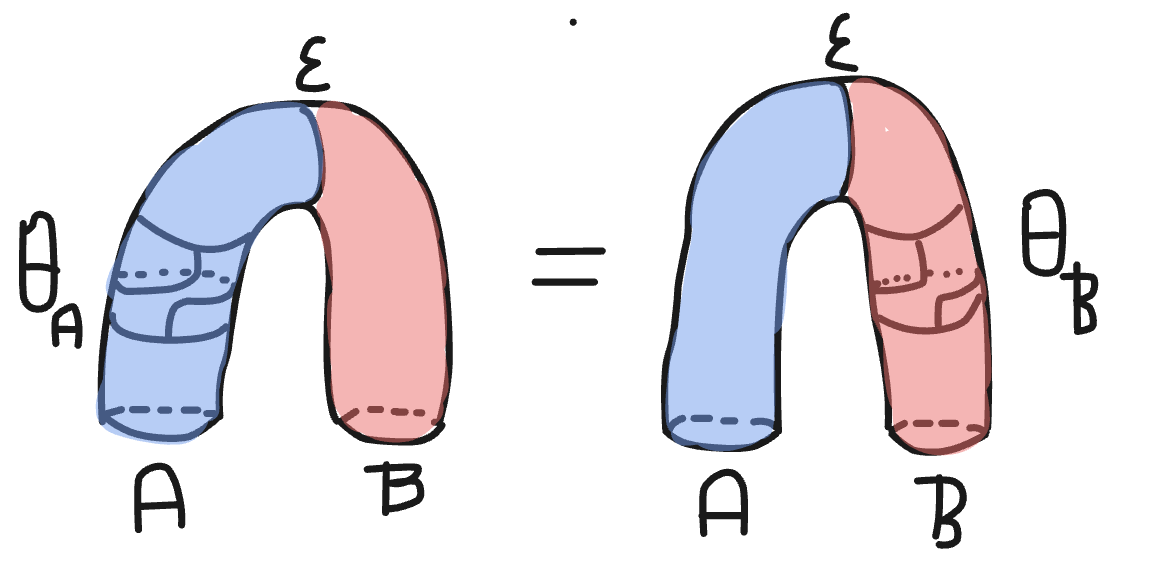
\includegraphics[scale=0.3]{blue-red-15.png}
  \end{center}

One can also observe the opposite category ${\mathcal{V}^{op}}^{(0,1)}$ of a balanced monoidal category $\mathcal{V}$ is also balanced,
the twist and the braiding operations are inherited from $\mathcal{V}$. By ${\mathcal{V}^{op}}^{(0,1)}$, we mean that the orientations
of the tensor product and morphism are reserved. The transformation $\mathcal{V} \mapsto {\mathcal{V}^{op}}^{(0,1)}$ 
consists in applying a central symmetry to string diagrams. The exact pairing $A \dashv A^*$ induces a monoidal functor
$(.) : \mathcal{V} \to {\mathcal{V}^{op}}^{(0,1)}$ transporting the ribbon structure to the ribbon structure.
Therefore, every exact pairing $A \dashv A^*$ in $\mathcal{V}$ defines an exact pairing $A \dashv A^*$ in ${\mathcal{V}^{op}}^{(0,1)}$
with unit defined as the image $\varepsilon^*_A : I \to A^* \otimes^{op} A$ of the counit $\varepsilon_A$. Therefore, a ribbon structure
on $\mathcal{V}$ induces the ribbon structure on ${\mathcal{V}^{op}}^{(0,1)}$.

Let $(A, B)$ a Frobenius pair in a ribbon category. The monoidal structure of $(.)^*$ sends the comonoid structure on $B$ to the monoid structure
on $B^*$. The resulting monoid structure $(B^*, d^*, u^*)$ can be constructed from either the exact pairing $B^* \dashv B$ or from the exact pairing
$B \dashv B^*$. Therefore, the monoid $(B^*, d^*, u^*)$ is involved in two exact pairing with the comonoid $(B, d, u)$ as a left and as a right dual:
\begin{center}
  $(B^*, d^*, u^*) \dashv (B, d, u)$

  $(B, d, u) \dashv (B^*, d^*, u^*)$
\end{center}
with unit $\eta_B$ and counit $\varepsilon_B$ and unit $\eta'_B$ and counit $\varepsilon'_B$ respectively. 
Let us compare those exact pairings between $(A, m, e)$ and $(B, d, u)$ involved in the definition of a Frobenius pair:
\begin{center}
  $(A, m, e) \dashv (B, d, u)$

  $(B, d, u) \dashv (A, m, e)$
\end{center}
with unit $\eta$ and counit $\varepsilon$ and unit $\eta'$ and counit $\varepsilon'$ respectively. Each comparison
induces a monoid isomorphism of $(A, m, e)$ with $(B^*, d^*, u^*)$ defined as:

\begin{center}
  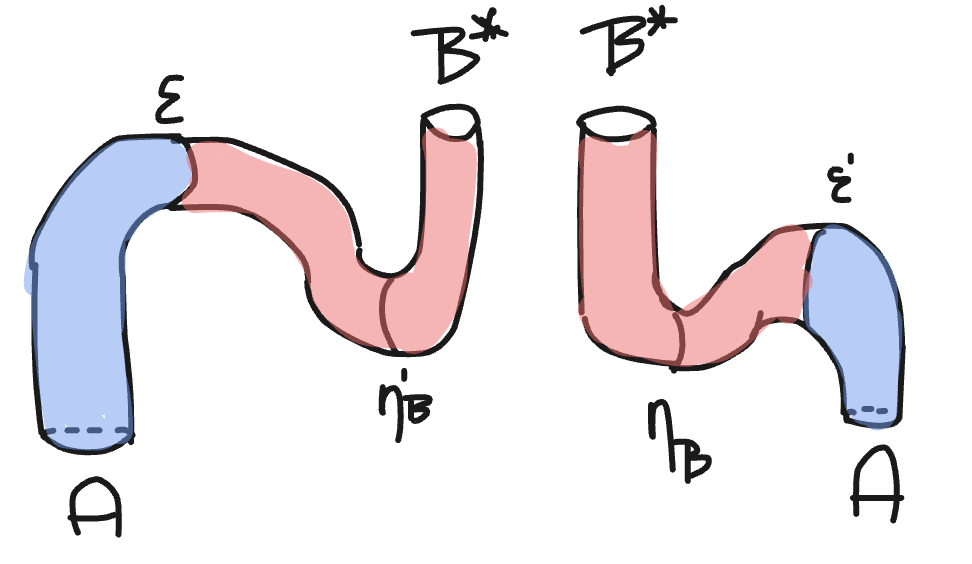
\includegraphics[scale=0.35]{blue-red-16.png}
\end{center}

The point is that the two isomorphisms $A \to B^*$ coincide exactly when a Frobenius pair $(A, B)$ is helical.
In this case, one obtains the following isomorphisms:
\[
\begin{tikzcd}
(A, m, e) \ar[rr, shift left=1.25ex, "(.)^{*}", ""{name=Fl}] && (B^*, d^*, u^*) \ar[ll, shift left=1.25ex, "{}^{*}(.)", ""{name=Fr}]
\end{tikzcd}
\] 
where $(.)^{*} : A \to B^*$ and ${}^{*}(.) : B^* \to A$ are isomorphisms defined as:
\begin{center}
  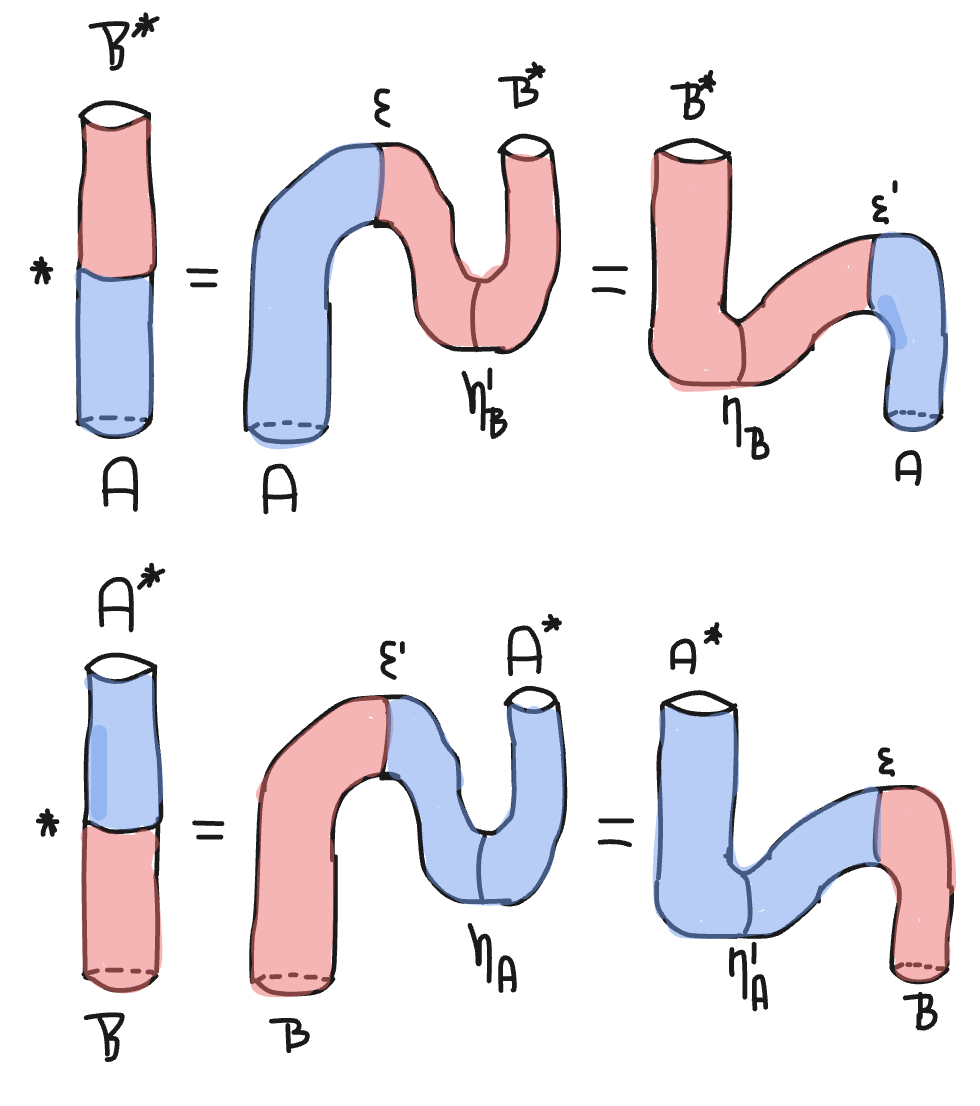
\includegraphics[scale=0.42]{blue-red-17.png}
\end{center}

From the definitions, we also conclude the following equalities:
\begin{center}
  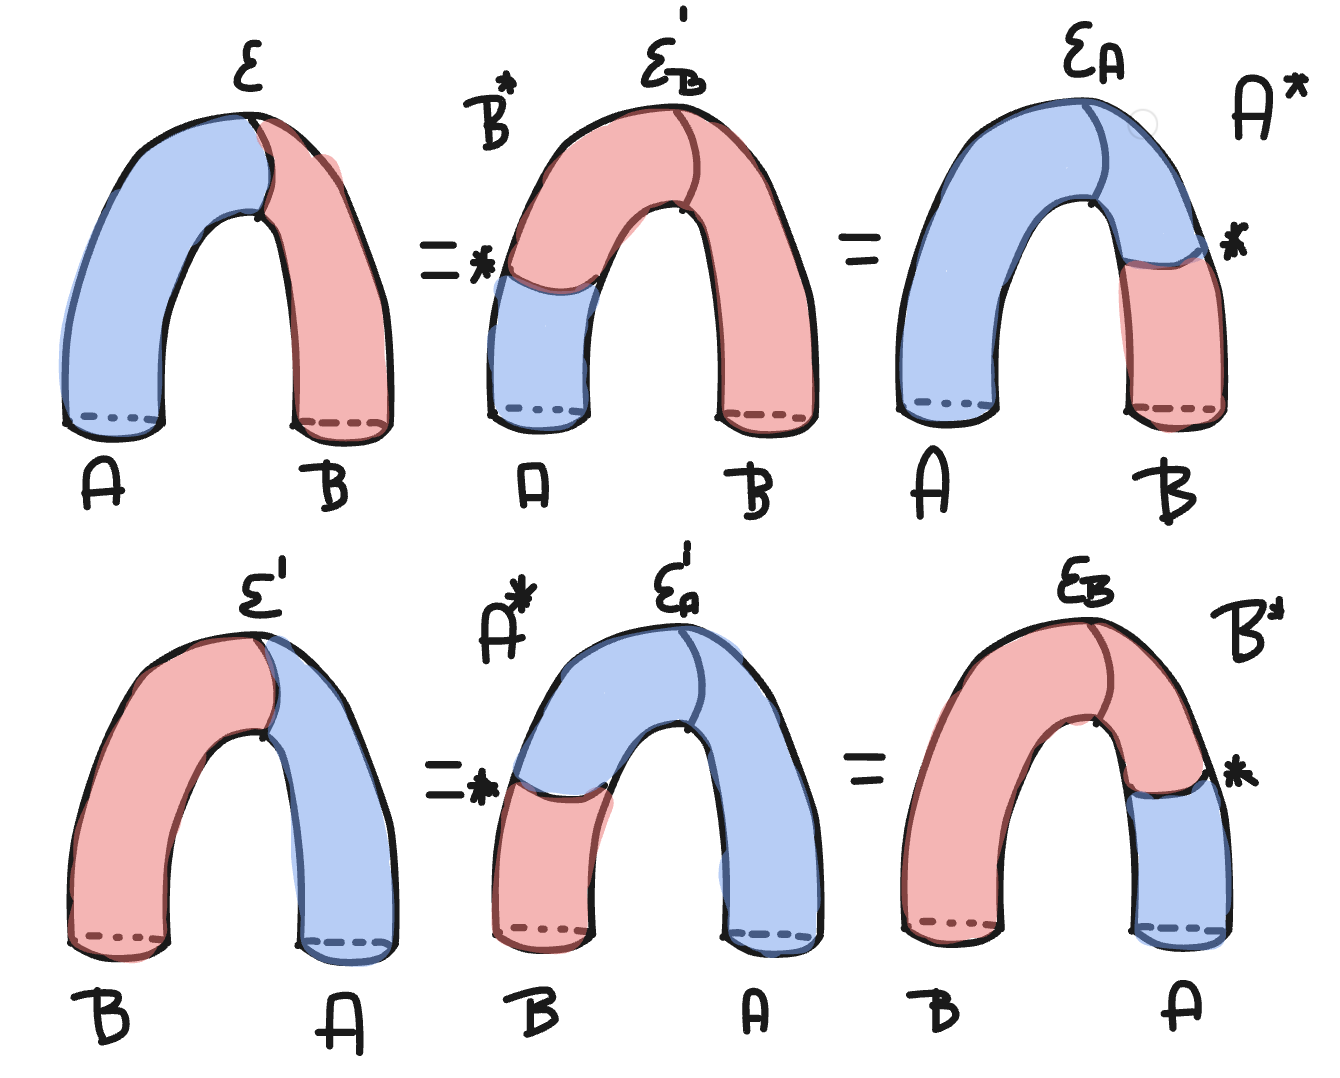
\includegraphics[scale=0.37]{blue-red-18.png}
\end{center}

Those equalities imply the following equivalent definition

\begin{prop}
  A helical Frobenius pair $(A, B)$ in a ribbon category is the same thing as a monoid $(A, m, e)$ and a comonoid $(B, d, u)$ equipped
  with a monoid isomorphism $(.)^* : (A, m, e) \to (B^*, d^*, u^*)$ and an isomorphism $L : A \to B^*$ such that the following equalities
  are satisfied:
  \begin{center}
  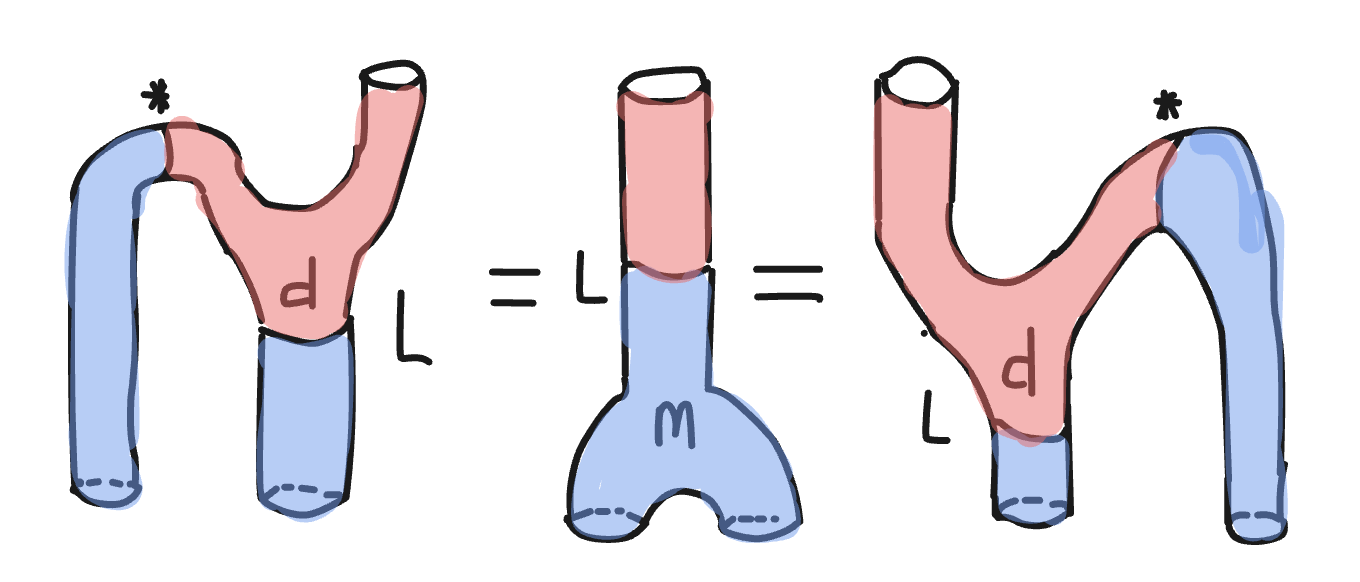
\includegraphics[scale=0.3]{blue-red-19.png}
  \end{center}
\end{prop}

\section{Dialogue Categories and Chiralities}

\begin{definition}
  A dialogue category is a monoidal category $(\mathcal{C}, \otimes, e)$ equipped with an object $\bot$ along with a family
  of isomorphisms
  \[
  \varphi_{x,y} : \mathcal{C}(x \otimes y, \bot) \cong \mathcal{C}(y, x \multimap \bot)
  \]
  natural in $x$ and $y$; along with a family of isomorphisms
  \[
  \psi_{x, y} : \mathcal{C}(x \otimes y, \bot) \cong \mathcal{C}(x, \bot \multimapinv y)
  \]
  natural in $x$ and $y$ as well.
\end{definition}

\begin{definition}
  A helical dialogue category is a dialogue category $\mathcal{C}$ equipped with a family of bijections natural in $x$ and $y$
  \[
  \operatorname{wheel}_{x,y} : \mathcal{C}(x \otimes y, \bot)
  \]
  such that the following diagram commutes for each $x, y, z \in \mathcal{C}$:
  \[
  \begin{tikzcd}
    \mathcal{C}((y \otimes z) \otimes x, \bot) \ar[rr, "\cong"] && \mathcal{C}(y \otimes (z \otimes x), \bot) \ar[dd, "\operatorname{wheel}_{y,z\otimes x}"] \\
    \\
    \mathcal{C}(x \otimes (y \otimes z), \bot) \ar[dd, "\cong"'] \ar[uu, "\operatorname{wheel}_{x,y\otimes z}"] && \mathcal{C}((z \otimes x) \otimes y, \bot) \\
    \\
    \mathcal{C}((x \otimes y) \otimes z, \bot) \ar[rr, "\operatorname{wheel}_{x \otimes y, z}"'] && \mathcal{C}(z \otimes (x \otimes y), \bot) \ar[uu, "\cong"']
  \end{tikzcd}
  \]
\end{definition}
Graphically, $\operatorname{wheel}_{x,y}$ is visualised as:
  \begin{center}
  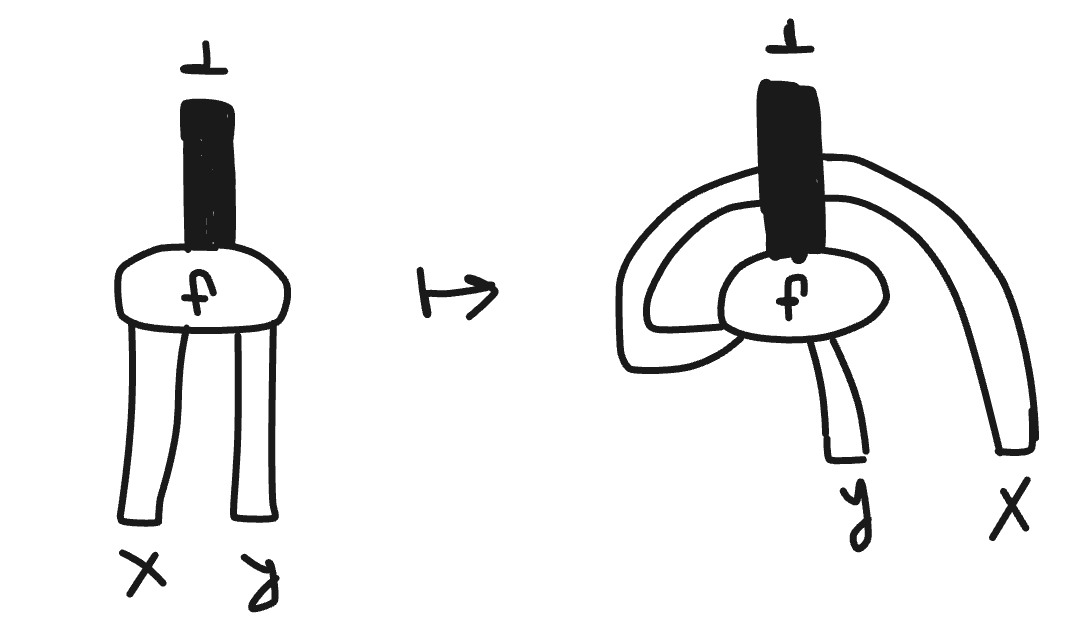
\includegraphics[scale=0.3]{wheel.png}
  \end{center}

\begin{definition}
  A helical chirality is a pair of monoidal categories $(\mathcal{A}, \circwedge, true)$ and $(\mathcal{B}, \circvee, false)$
  equipped with a monoidal equivalence and an adjunction respectively:
  \[
  \begin{tikzcd}
  \mathcal{A} \ar[rr, shift left=1.25ex, "(.)^*", ""{name=Fl}] && \mathcal{B} \ar[ll, shift left=1.25ex, "{}^{*}(.)", ""{name=Fr}]
  \end{tikzcd}
  \]
  \[
  \begin{tikzcd}
  \mathcal{A} \ar[rr, shift left=1.25ex, "L", ""{name=Fl}] && \mathcal{B} \ar[ll, shift left=1.25ex, "R", ""{name=Fr}]
  \arrow[phantom, from=Fr, to=Fl, "\dashv" rotate=-90]
  \end{tikzcd}
  \]
  with the following isomorphisms:
  \[
  \chi^{L}_{m,a,b} : \langle m \circwedge a \: | \: b \rangle \to \langle a \: | \: m^* \circvee b \rangle
  \]
  \[
  \chi^{R}_{m,a,b} : \langle a \circwedge m \: | \: b \rangle \to \langle a \: | \: b \circvee m^* \rangle
  \]
  where $\langle . | . \rangle := \mathcal{A}(., R(.)) : \mathcal{A}^{op} \times B \to Set$ is the evaluation bracket.
  The currified combinators $\chi^{L}$ and $\chi^R$ satisfy the following diagrams for each $m, n, a \in \mathcal{A}$ and for $b \in \mathcal{B}$:
  \[
  \begin{tikzcd}
  \langle (m \circwedge n) \circwedge a \: | \: b \rangle \ar[d, "\cong"'] \ar[rrrr, "\chi^L_{m \circwedge n}"] &&&& \langle a \: | \: (m \circwedge n)^* \circvee b \rangle  \\
  \langle m \circwedge (n \circwedge a) \: | \: b \rangle \ar[rr, "\chi^L_m"'] && \langle n \circwedge a \: | \: m^* \circvee b \rangle \ar[rr, "\chi^L_n"'] && \langle a \: | \: n^* \circvee m^* \circvee b \rangle \ar[u, "\cong"']
  \end{tikzcd}
  \]
  \[
  \begin{tikzcd}
  \langle a \circwedge (m \circwedge n) \: | \: b \rangle \ar[d, "\cong"'] \ar[rrrr, "\chi^R_{m \circwedge n}"] &&&& \langle a \: | \: b \circvee (m \circwedge n)^* \rangle  \\
  \langle (a \circwedge m) \circwedge n \: | \: b \rangle \ar[rr, "\chi^R_n"'] && \langle a \circwedge m \: | \: b \circvee n^* \rangle \ar[rr, "\chi^R_m"'] && \langle a \: | \: (b \circvee n^*) \circvee m^* \rangle \ar[u, "\cong"']
  \end{tikzcd}
  \]
  \[
  \begin{tikzcd}
    \langle (m \circwedge a) \circwedge n \: | \: b \rangle \ar[d, "\cong"'] \ar[rr, "\chi^R_n"] && \langle m \circwedge a \: | \: b \circvee n^* \rangle  \ar[rr, "\chi^R_n"] && \langle a \: | \: m^* \circvee (b \circvee n^*) \rangle \ar[d, "\cong"] \\
    \langle m \circwedge (a \circwedge n) \: | \: b \rangle \ar[rr, "\chi^L_m"'] && \langle a \circwedge n \: | \: m^* \circvee b \rangle \ar[rr, "\chi^R_n"'] && \langle a \: | \: (m^* \circvee b) \circvee n^* \rangle \\
  \end{tikzcd}
  \]
\end{definition}

Every helical dialogue category $\mathcal{C}$ induces defines a helical dialogue chirality by taking
$\mathcal{A} = \mathcal{C}$, $\mathcal{B} = \mathcal{C}^{op^{(0,1)}}$, $La := a \multimap \bot$, 
$Rb := \bot \multimapinv b$. The right currification of the combinator $\chi^R$ is simply defined
by using the dialogue structure of the category $\mathcal{C}$:
\[
\langle a \circwedge m \: | \: b \rangle = \mathcal{C}(a \otimes m, \bot \multimapinv b) \xrightarrow{\psi^{-1}_{a \otimes m, b}} \mathcal{C}(a \otimes m \otimes b, \bot) \xrightarrow{\psi_{a, m \otimes b}} \mathcal{C}(a, \bot \multimapinv m \otimes b) = \langle a | b \circvee m^* \rangle 
\]
The left currification $\chi^L$ requires the helical structure:
\[
\begin{array}{lll}
& \langle m \circwedge a \: | \: b \rangle = \mathcal{C}(m \circwedge a, \bot \multimapinv b) \xrightarrow{\psi^{-1}_{m \otimes a, b}} \mathcal{C}(m \otimes a \otimes b, \bot) \xrightarrow{\operatorname{wheel}_{m, a \otimes b}}& \\ 
& \:\:\:\: \mathcal{C}(a \otimes b \otimes m, \bot) \xrightarrow{\psi_{m \otimes b, a}} \mathcal{C}(a, \bot \multimapinv b \otimes m) = \langle a \: | \: m^* \circvee b \rangle &
\end{array}
\]

\section{Categorical Bimodules}

Let $\mathcal{A}$ and $\mathcal{B}$ be categories, an $\mathcal{A}\mathcal{B}$-module $M$ is defined as a bifunctor
$M : \mathcal{A}^{op} \times \mathcal{B} \to \operatorname{Set}$. The bicategory (a weak 2-category) ${\bf BiMod}$ of bimodules consists of
the following data:
\begin{itemize}
  \item small categories as 0-cells,
  \item $\mathcal{A}\mathcal{B}$-modules $M$ as 1-cells $M : A \to B$,
  \item natural transformations $\theta : N \Rightarrow M : \mathcal{A}^{op} \times \mathcal{B} \to \operatorname{Set}$ as 2-cells
  $\theta : M \Rightarrow N : \mathcal{A} \to \mathcal{B}$.
\end{itemize}
The orientation of 2-cells allows defining a 2-monoidal functor ${\bf Cat} \to {\bf BiMod}$ transporting every functor
$F : \mathcal{A} \to \mathcal{B}$ to the bimodule:
\[
F_{\bullet} : (a, b) \mapsto \mathcal{A}(Fa, b)
\]
One can view ${\bf BiMod}$ as a 2-dimensional Kleisli construction on the small limit completion 
$\mathcal{C} \mapsto [\mathcal{C}, \operatorname{Set}]^{op}$. One can recover the more familiar
convention corresponding to the small colimit completion $\mathcal{C} \mapsto [\mathcal{C}^{op}, \operatorname{Set}]$
by taking the bicategory ${\bf BiMod}^{op^{(1,2)}}$ obtained from ${\bf BiMod}$ by reversing 1 and 2-cells.

There is also a monoidal 2-functor ${\bf Cat} \to {\bf BiMod}^{op^{(1,2)}}$ defined as follows. First of all,
the operation $(.)^{op} : \mathcal{C} \mapsto \mathcal{C}^{op}$ defines a 2-functor 
${\bf Cat} \to {\bf Cat}^{op^{(1,2)}}$. ${\bf BiMod}$ is also symmetric monoidal with $\otimes = \times$. 
It is also autonomous, and its ribbons are trivial.
There exists a 2-monoidal functor $(.)^* : {\bf BiMod} \to {\bf BiMod}^{op^{(0,1)}}$ transporting every $A$
to its dual $A^*$. $A^*$ happens to coincide with $A^{op}$. Therefore, one has a 2-monoidal functor:
\[
{\bf Cat} \xrightarrow{op} {\bf Cat}^{op^{(0,1)}} \rightarrow {\bf BiMod}^{op^{(2)}} \xrightarrow{*} {\bf BiMod}^{op^{(1,2)}}
\]
transporting every category $\mathcal{A}$ to itself and every $F : \mathcal{A} \to \mathcal{B}$ to the bimodule
\[
F^{\bullet} : (a, b) \mapsto \mathcal{A}(a, Fb)
\]
$F^{\bullet}$ is also left adjoint to $F_{\bullet}$ in ${\bf BiMod}$.

\section{Frobenius Pseudomonoids}

The concept of a Frobenius pseudomonoid reflects the properties of a dialogue category $\mathcal{A}$
transported from ${\bf Cat}$ to the monoidal bicategory ${\bf BiMod}$.

\begin{definition}
  A lax pairing $\mathcal{A} \dashv \mathcal{B}$ in a monoidal bicategory consists of a pair of
  1-cells $\eta_{[1]} : \mathcal{A} \otimes \mathcal{B} \to I$ and 
  $\varepsilon_{[1]} : \mathcal{B} \otimes \mathcal{A} \to I$ along with a pair of 2-cells:
  \begin{center}
  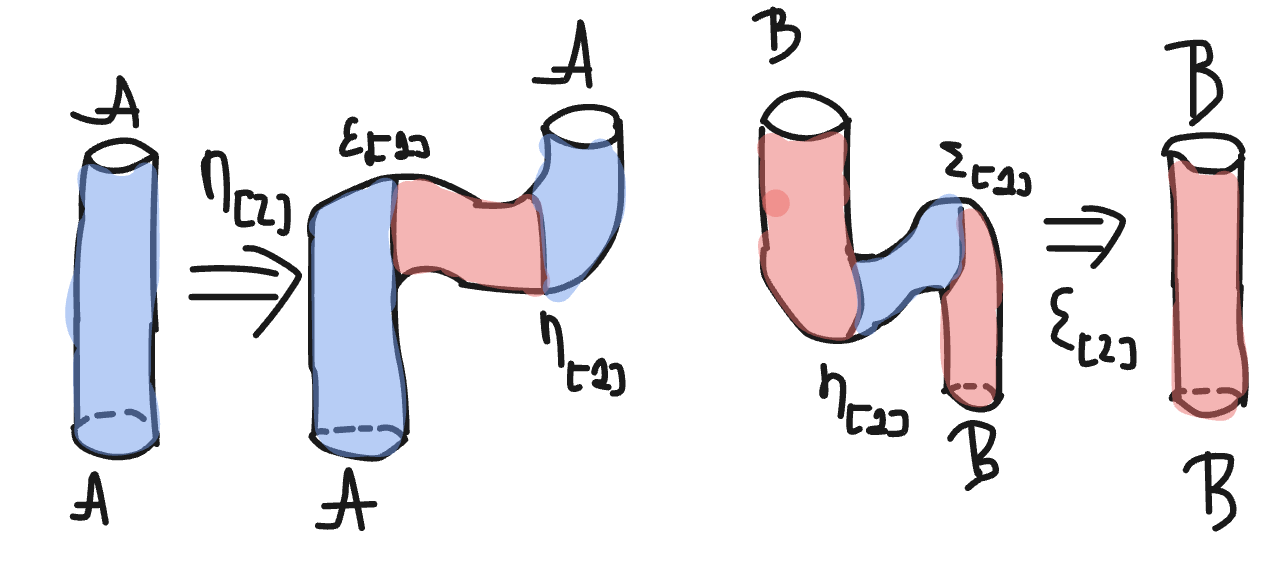
\includegraphics[scale=0.4]{blue-red-20.png}
  \end{center}
  such that the following composite 2-cell
  \begin{center}
  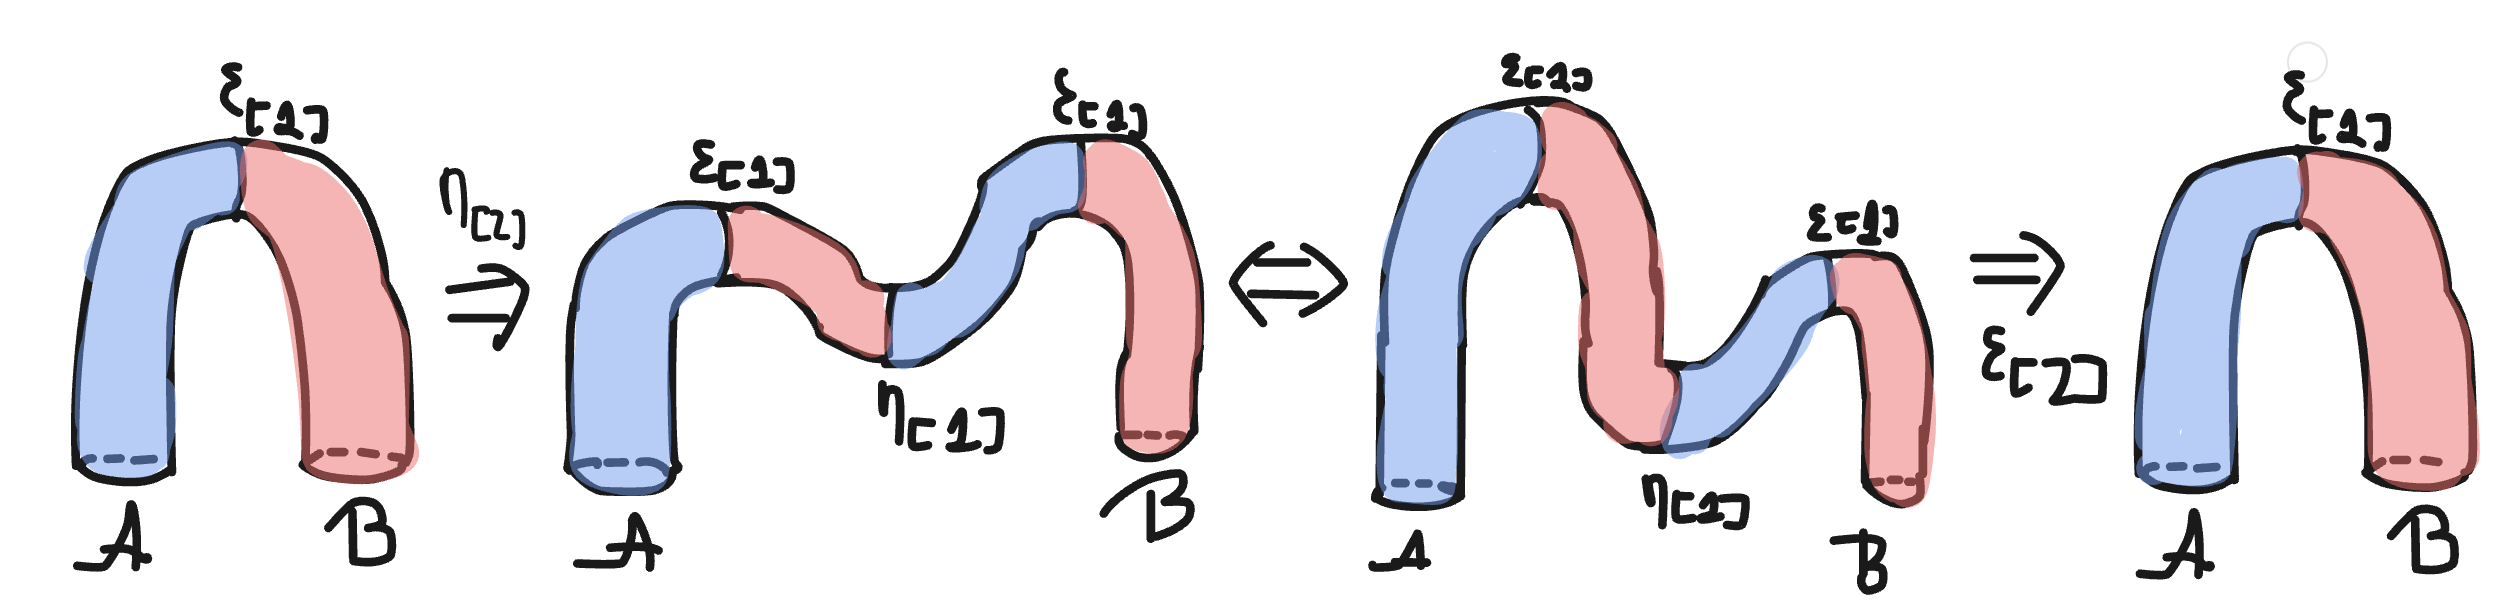
\includegraphics[scale=0.36]{blue-red-21.png}
  \end{center}
  coincides with the identity on the 1-cell $\varepsilon_{[1]}$ and, symmetrically, the opposite 
  2-cell:
  \begin{center}
  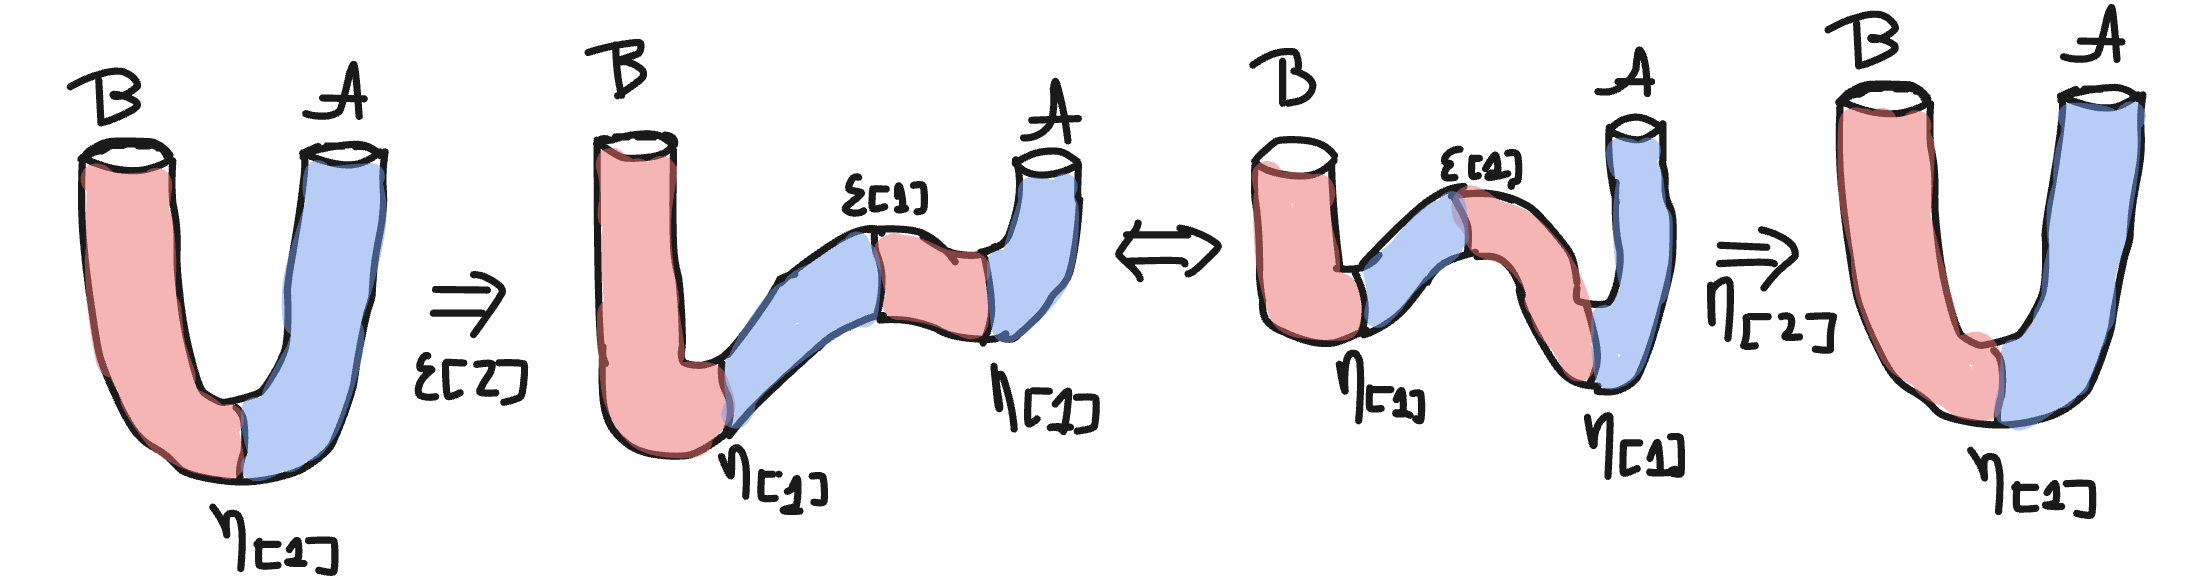
\includegraphics[scale=0.4]{blue-red-22.png}
  \end{center}
  coincides with the identity on the 1-cell $\eta_{[1]}$.
\end{definition}

\begin{definition}
  A \emph{Frobenius form} on a pseudomonoid $\mathcal{A}$ is a monoidal bicategory is a lax pairing 
  $\mathcal{A} \dashv \mathcal{A}$ equipped with a 2-cell
  \begin{center}
  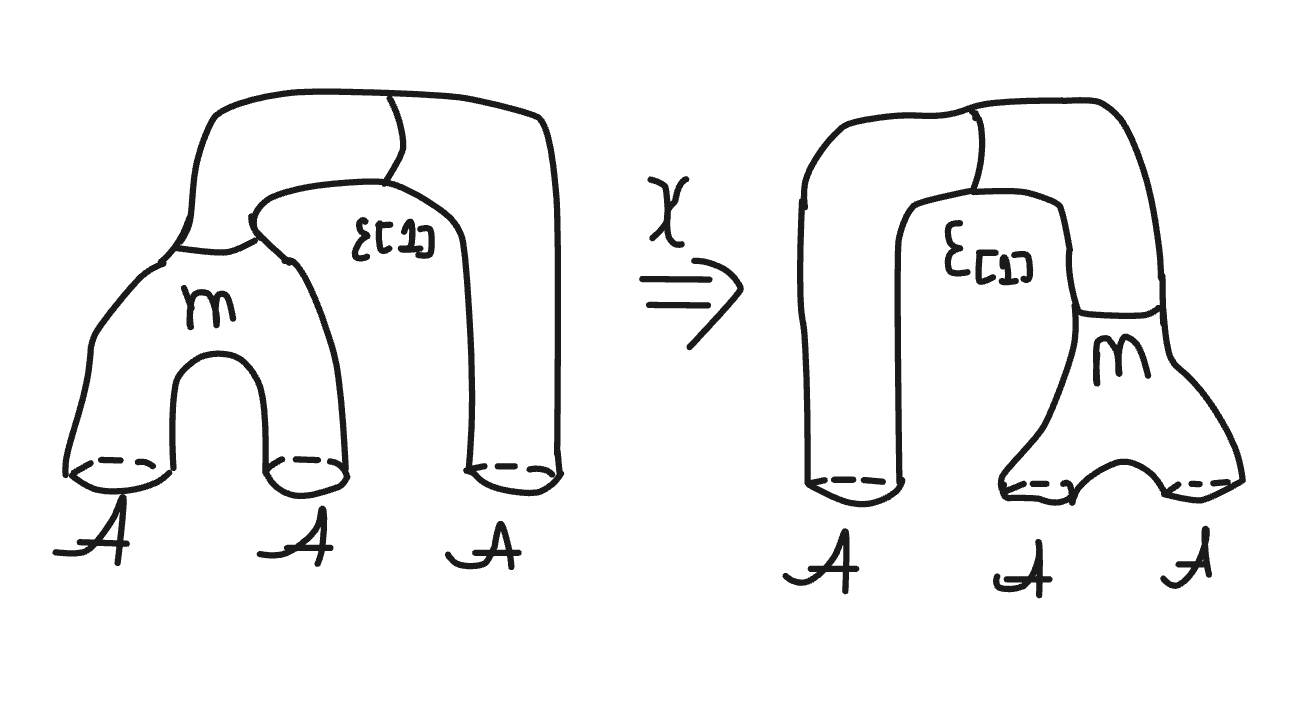
\includegraphics[scale=0.3]{frobenius-form-1.png}
  \end{center}
  called \emph{the associativity law of a Frobenius form} such that the following variation of 
  the MacLane pentagon is satisfied
  \begin{center}
  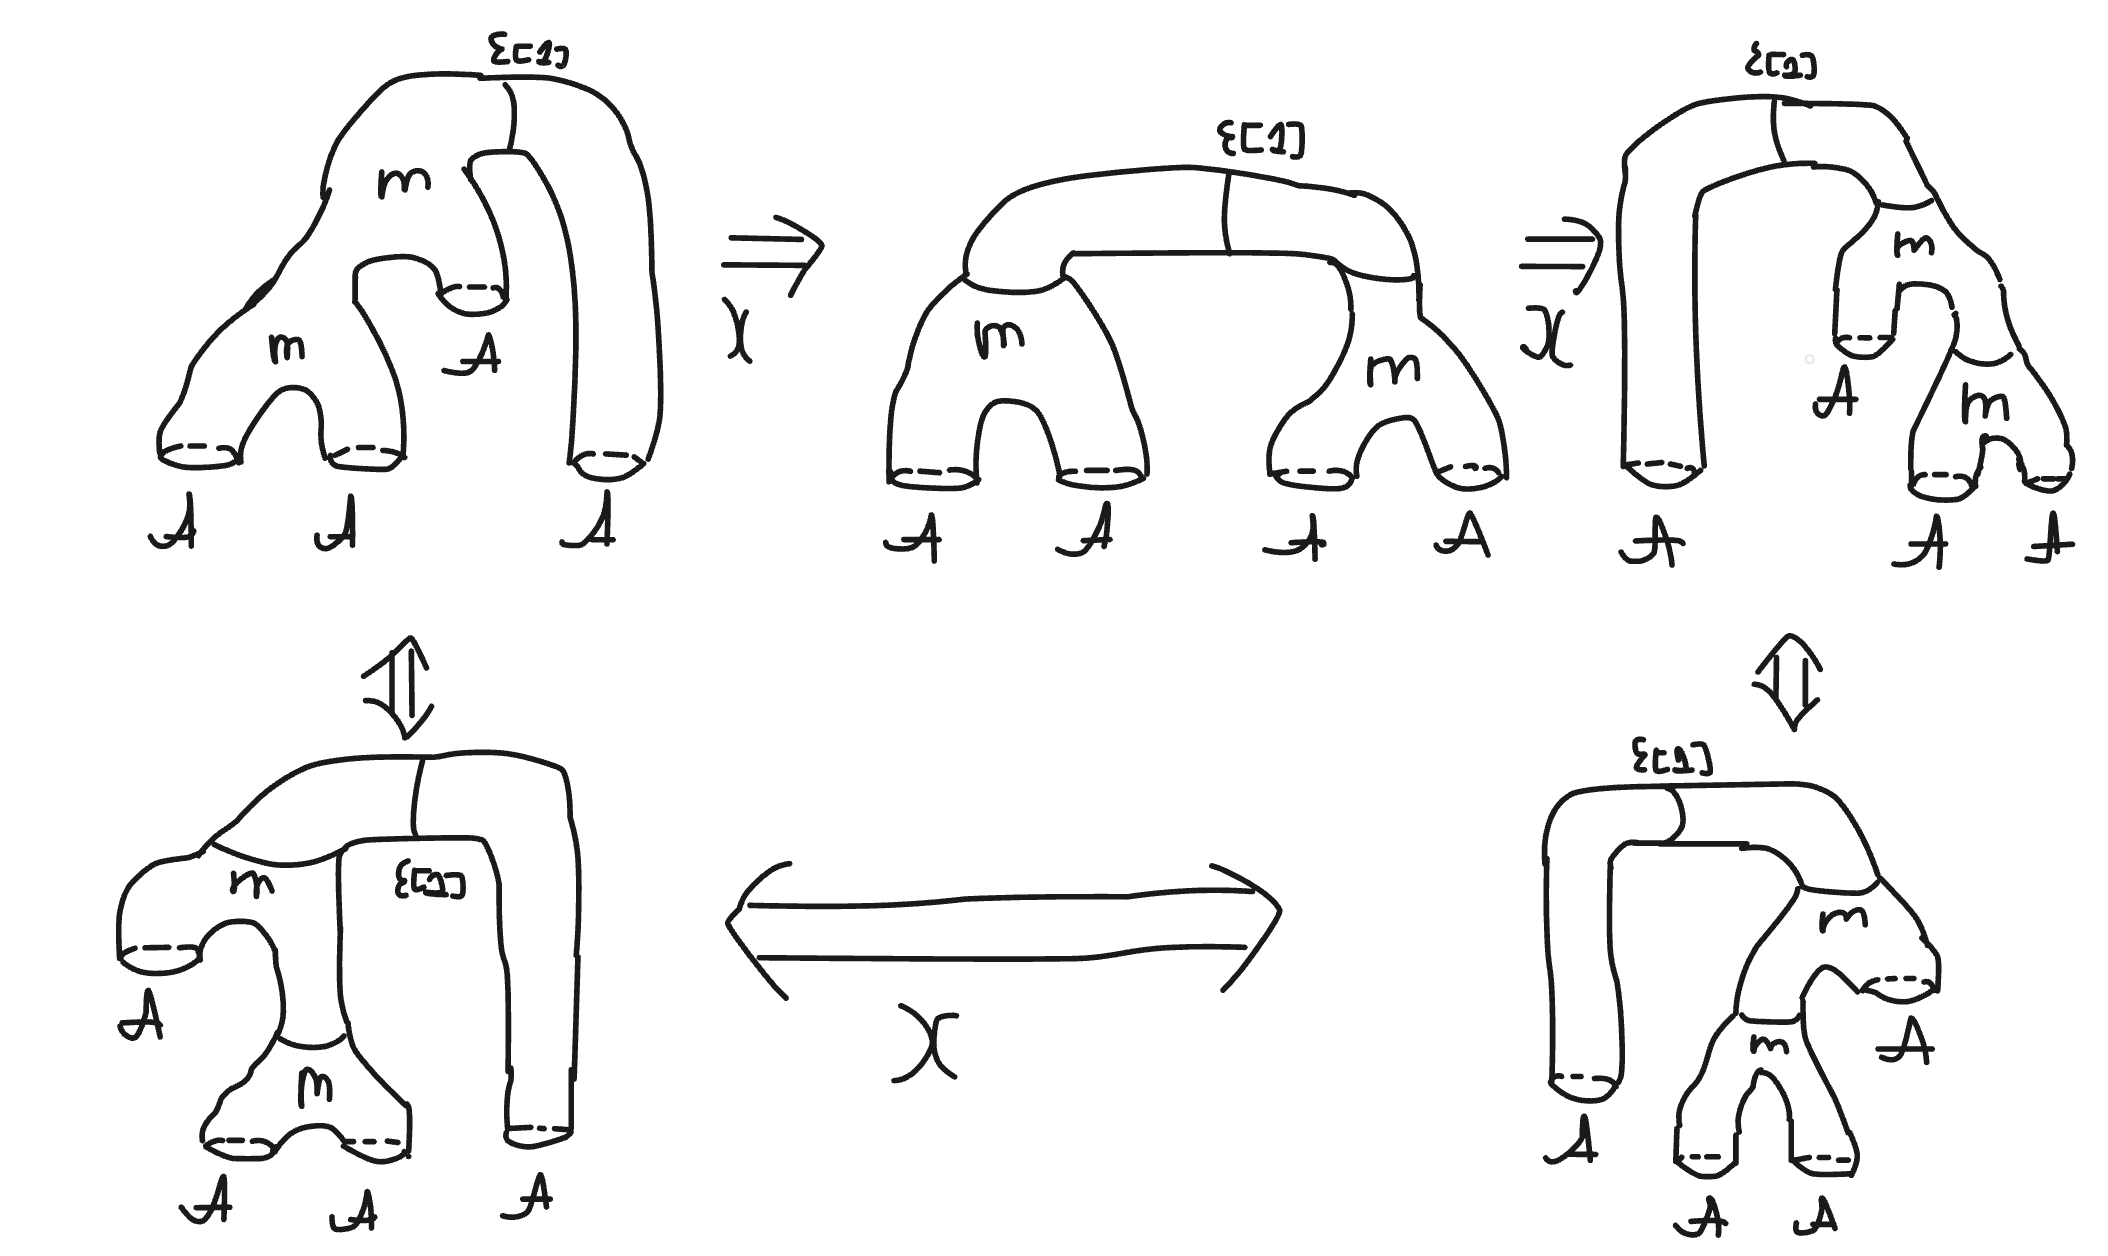
\includegraphics[scale=0.4]{frobenius-form-2.png}
  \end{center}

  A \emph{Frobenius pseudomonoid} is a pseudomonoid equipped with a Frobenius from.
\end{definition}

Observe that in ${\bf BiMod}$, every dialogue category $\mathcal{A}$ defined a Frobenius pseudomonoid with Frobenius form
defined as:
\begin{center}
  $\varepsilon_{[1]} : (a_1, a_2) \mapsto \mathcal{A}(a_1 \otimes a_2, \bot)$

  $\eta_{[1]} : (a_1, a_2) \mapsto \mathcal{A}(\bot \multimapinv a_1, a_2)$
\end{center}
and $\chi$ is defined by the associativity law from $\mathcal{A}$. 
But the above notion of Frobenius pseudomonoid does not coincide with the notion of a Frobenius monoid
when the underlying monoidal bicategory is a monoidal category with trivialised 2-cells.

\begin{definition} A ribbon structute on a lax pairing $\mathcal{A} \dashv \mathcal{B}$ in a balanced monoidal
  bicategory is a pair of invertible 2-cells
  \begin{center}
  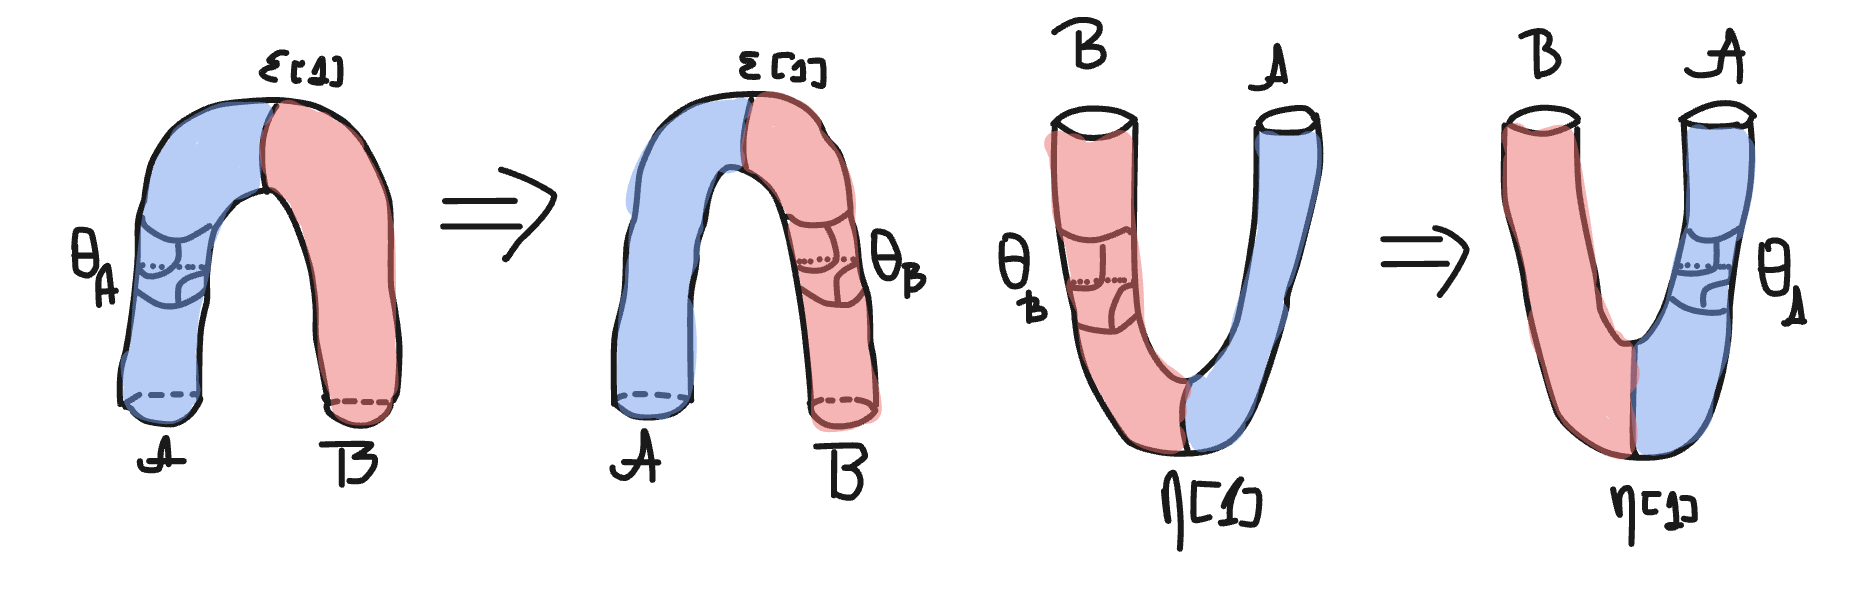
\includegraphics[scale=0.45]{blue-red-23.png}
  \end{center}
  such that both composite 2-cells
  \begin{center}
  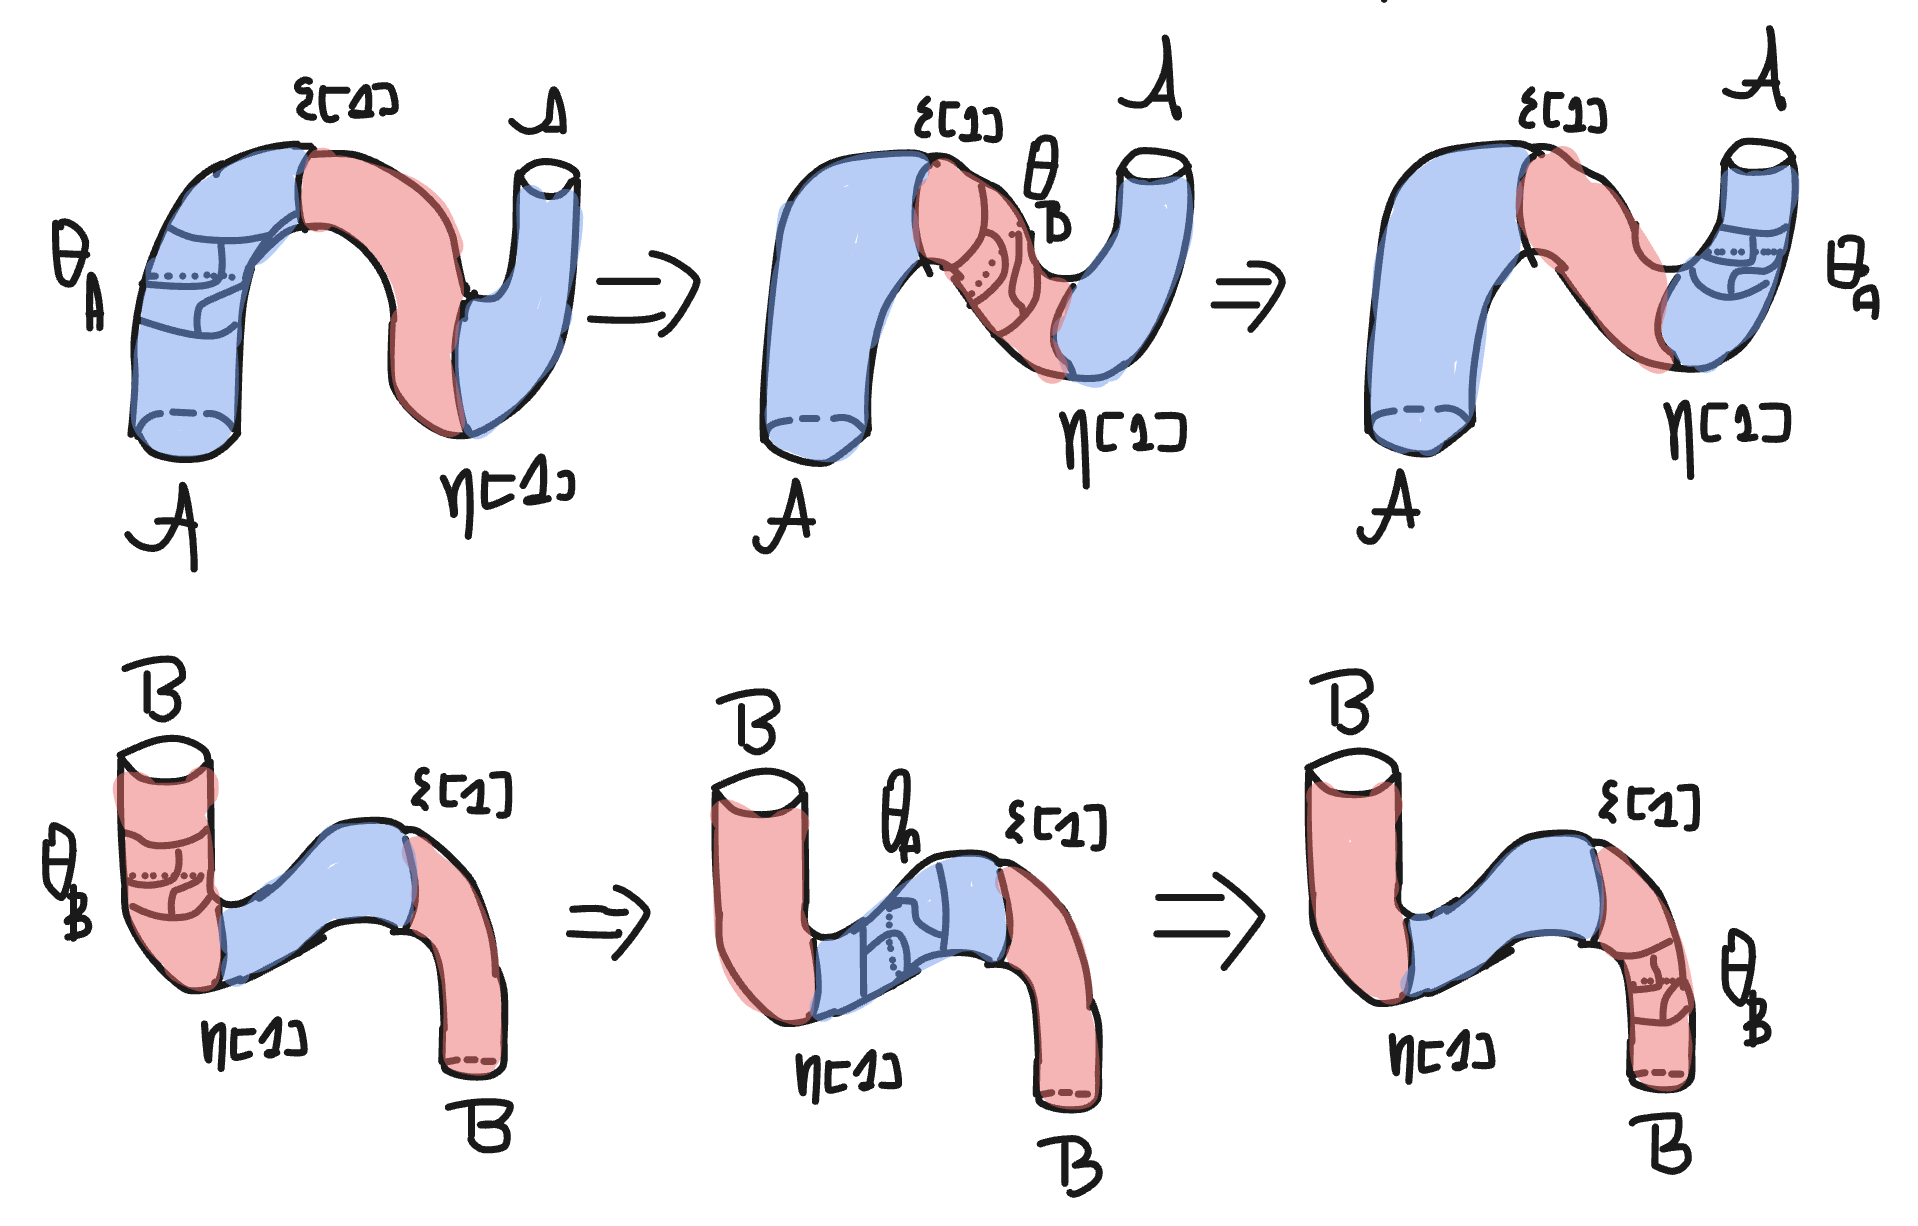
\includegraphics[scale=0.45]{blue-red-24.png}
  \end{center}
  coincide with the identity 2-cells.

  A \emph{lax ribbon pairing} is a lax pairing equipped with a pairing structure.
\end{definition}

\begin{definition}
  A helical Frobenius pseudomonoid in a balanced monoidal category is a Frobenius pseudomonoid
  whose lax pairing is equipped with a ribbon structure and the following invertible 2-cell:
  \begin{center}
  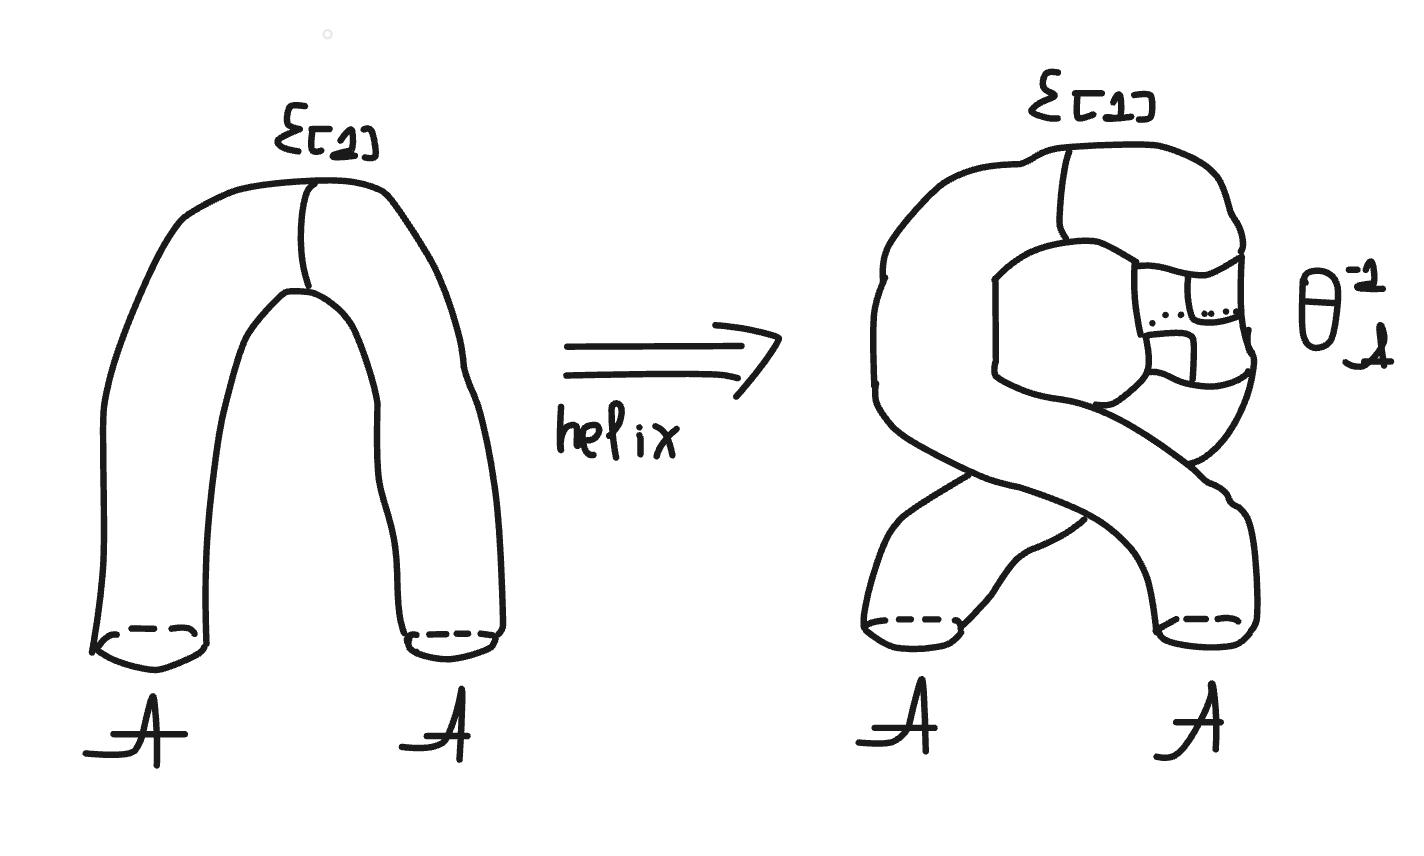
\includegraphics[scale=0.35]{helical-frobenius-pseudo.png}
  \end{center}

$\operatorname{helix}$ can be viewed as a 2-cell $||a_1, a_2|| \Rightarrow ||a_2, a_1||$ such that
the following commutes:
\[
\begin{tikzcd}
  {||a_1 \bullet a_2, a_3 ||} \ar[d, Rightarrow, "\operatorname{helix}"] \ar[rr, Rightarrow, "\chi"] && {||a_1, a_2 \bullet a_3 ||} \ar[rr, Rightarrow, "\operatorname{helix}"] && {||a_2 \bullet a_3, a_1 ||} \ar[d, Rightarrow, "\chi"] \\
  {||a_3, a_1 \bullet a_2 ||} && {||a_3 \bullet a_1, a_2||} \ar[ll, Rightarrow, "\chi"] && {||a_2, a_3 \bullet a_2||} \ar[ll, Rightarrow, "\operatorname{helix}"]
\end{tikzcd}
\]
\end{definition}
Every helical dialogue category $\mathcal{A}$ induces a Frobenius pseudomonoid in ${\bf BiMod}$ with $\operatorname{helix}$
defined as follows:
\[
\operatorname{helix}_{a_1, a_2} := \operatorname{wheel}^{-1}_{a_1, a_2} : \mathcal{A}(a_2 \otimes a_1, \bot) \Rightarrow \mathcal{A}(a_1 \otimes a_2, \bot)
\]

\section{Frobenius Amphimonoids}

\begin{definition}
  A \emph{biexact} pairing $\mathcal{A} \dashv \mathcal{B}$ is a lax pairing whose 2-cells 
  $\eta_{[2]}$ and $\varepsilon_{[2]}$ are reversible. A \emph{biexact ribbon pairing} is a biexact pairing with a ribbon structure.
\end{definition}

\begin{definition}
  An \emph{amphimonoid} $(\mathcal{A}, \mathcal{B})$ in a balanced monoidal bicategory $\mathcal{W}$
  is defined as a pseudomonoid $(\mathcal{A}, \circwedge, true)$ and a pseudocomonoid $(\mathcal{B}, \circvee, false)$
  equipped with biexact pairing $\mathcal{A} \dashv \mathcal{B}$ (noted as * below) and a pair of 2-cells:
  \begin{center}
  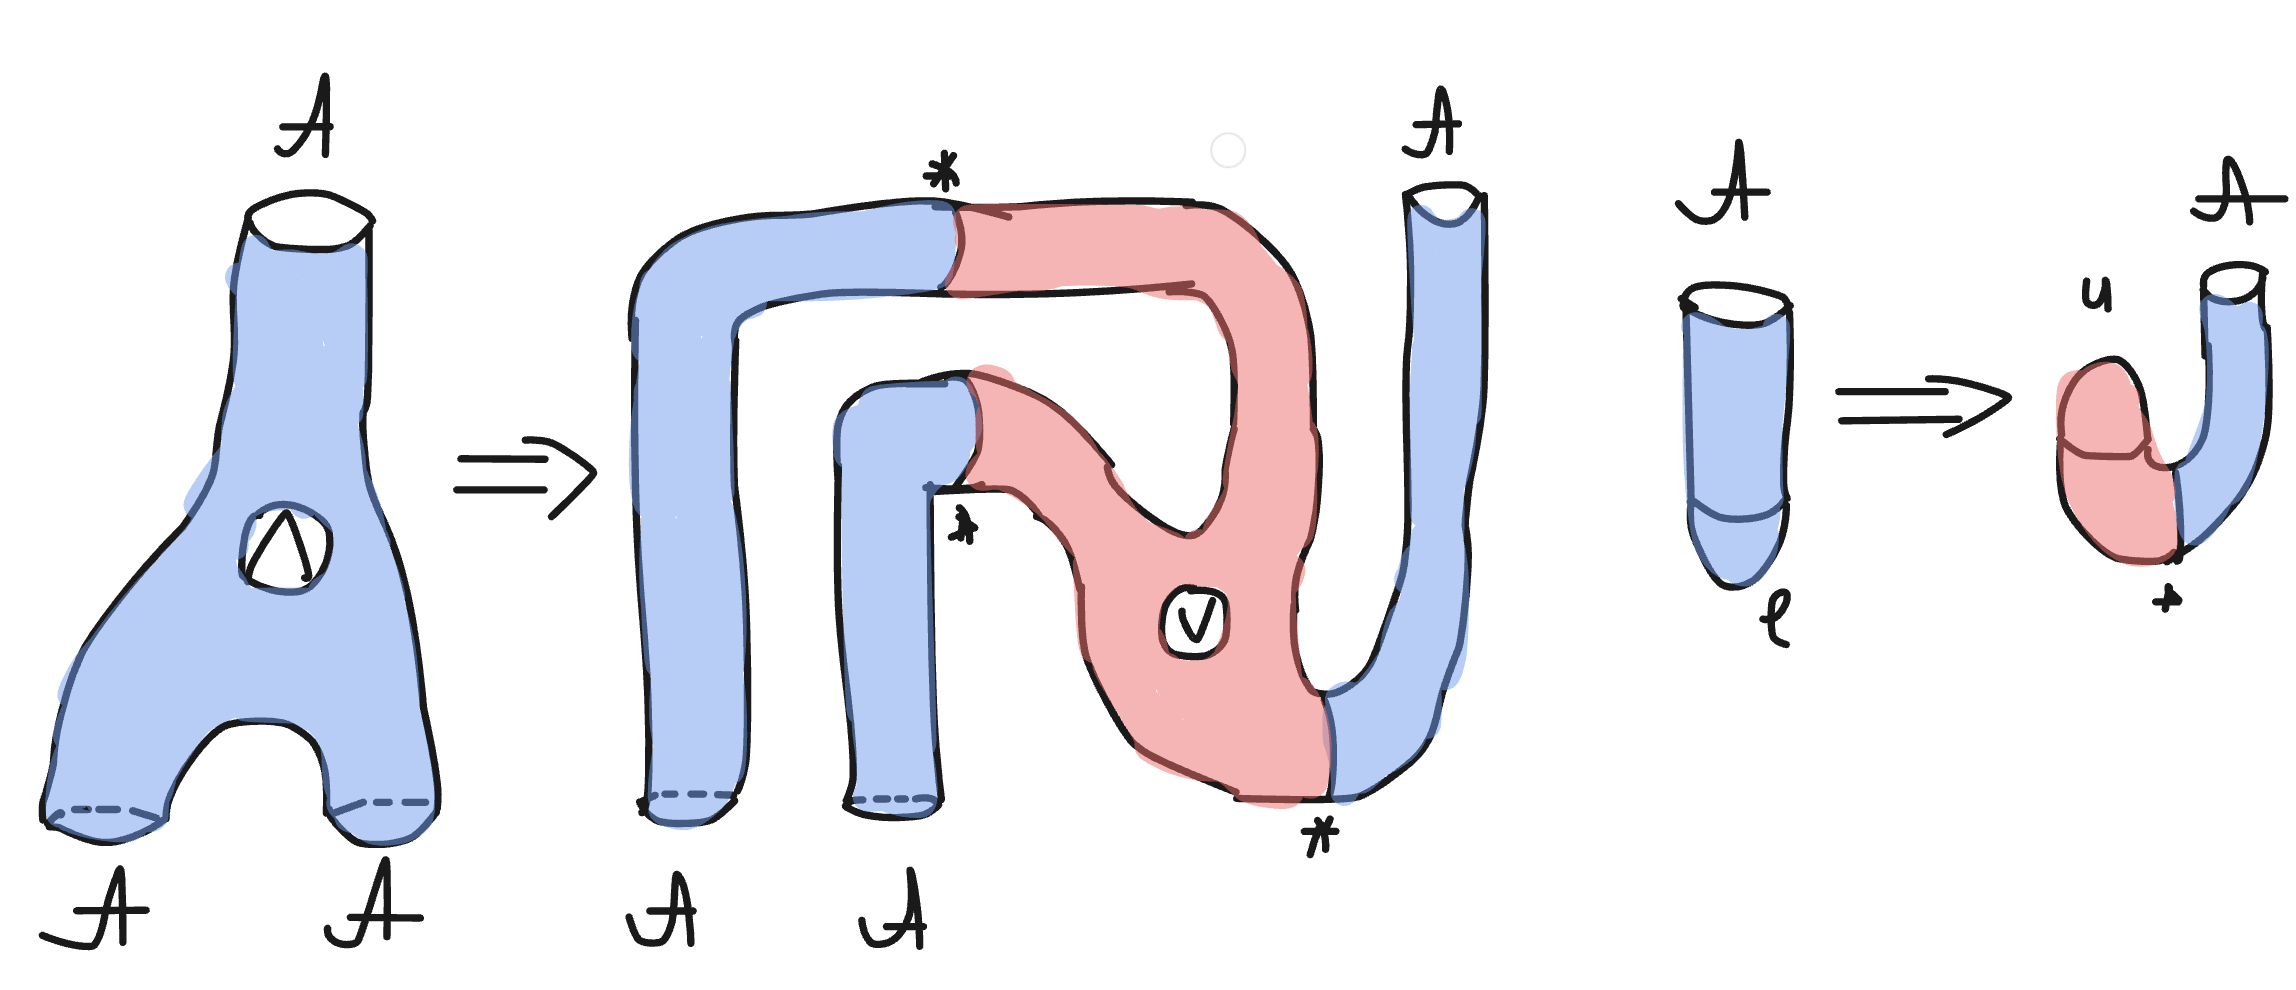
\includegraphics[scale=0.3]{blue-red-25.png}
  \end{center}
  establishing a pseudomonoid equivalence between $(\mathcal{A}, \circwedge, true)$ and a pseudomonoid on $\mathcal{B}$
  induced by the structure of a biexact pairing. 
\end{definition}

Moreover, every amphimonoid induces a biexact ribbon pairing $\mathcal{B} \dashv \mathcal{A}$ defined as follows:
  \begin{center}
  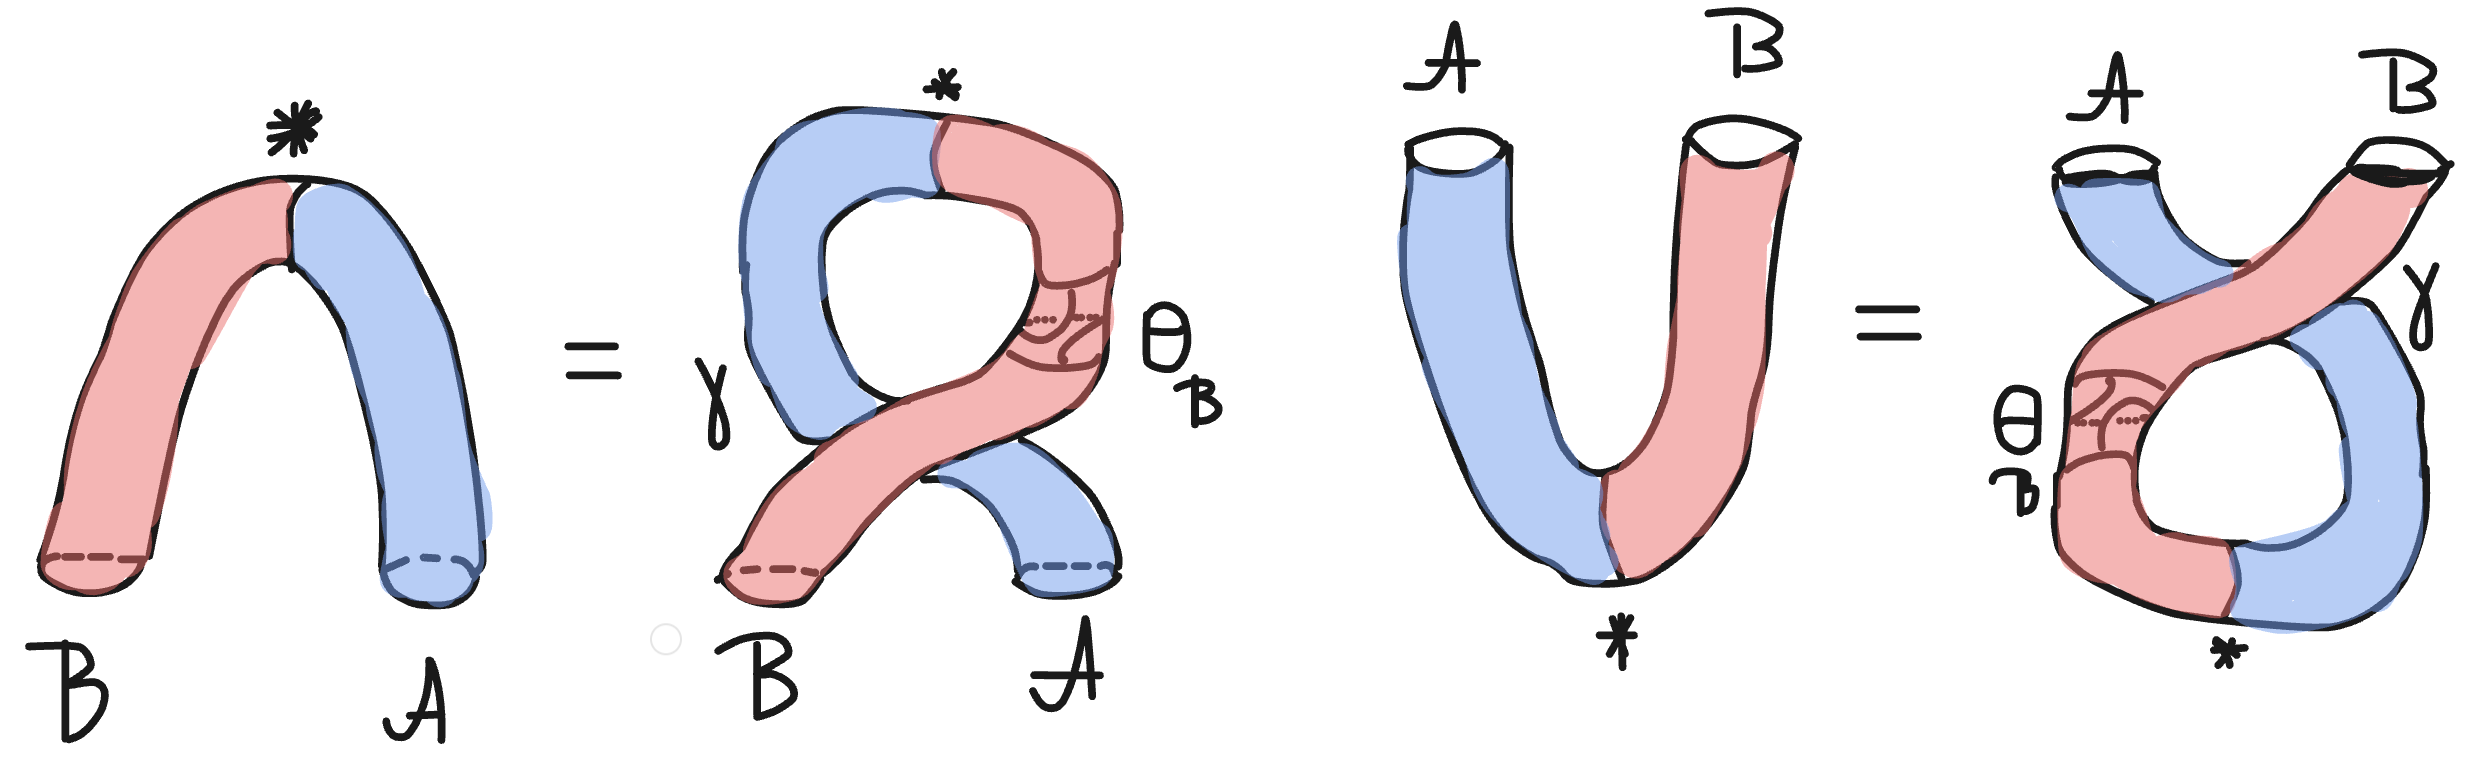
\includegraphics[scale=0.3]{blue-red-26.png}
  \end{center}
  along with a pair of invertible 2-cells
  \begin{center}
  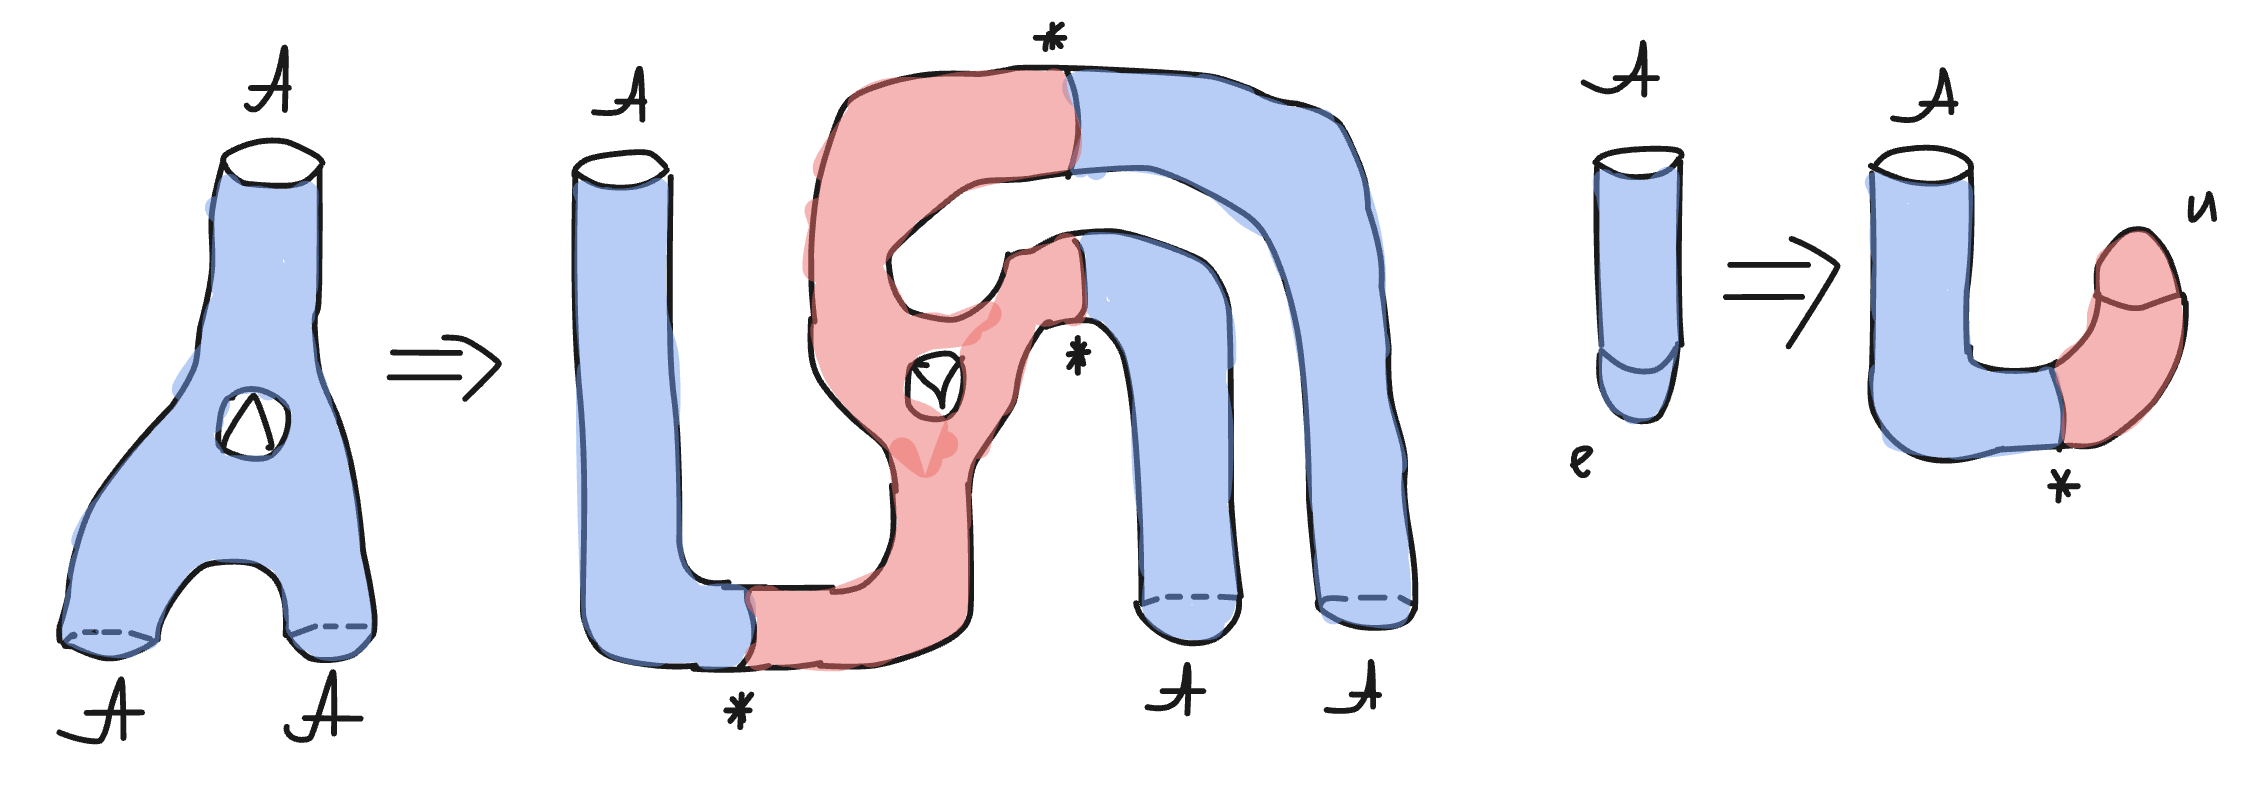
\includegraphics[scale=0.3]{blue-red-27.png}
  \end{center}

\begin{definition}
  A Frobenius amphimonoid $(\mathcal{A}, \mathcal{B}, L, R)$ consists of an amphimonoid $(\mathcal{A}, \mathcal{B})$
  along with an adjunction
  \[
  \begin{tikzcd}
  \mathcal{A} \ar[rr, shift left=1.25ex, "L", ""{name=Fl}] && \mathcal{B} \ar[ll, shift left=1.25ex, "R", ""{name=Fr}]
  \arrow[phantom, from=Fr, to=Fl, "\dashv" rotate=-90]
  \end{tikzcd}
  \]
  along with two inverible 2-cells
  \begin{center}
  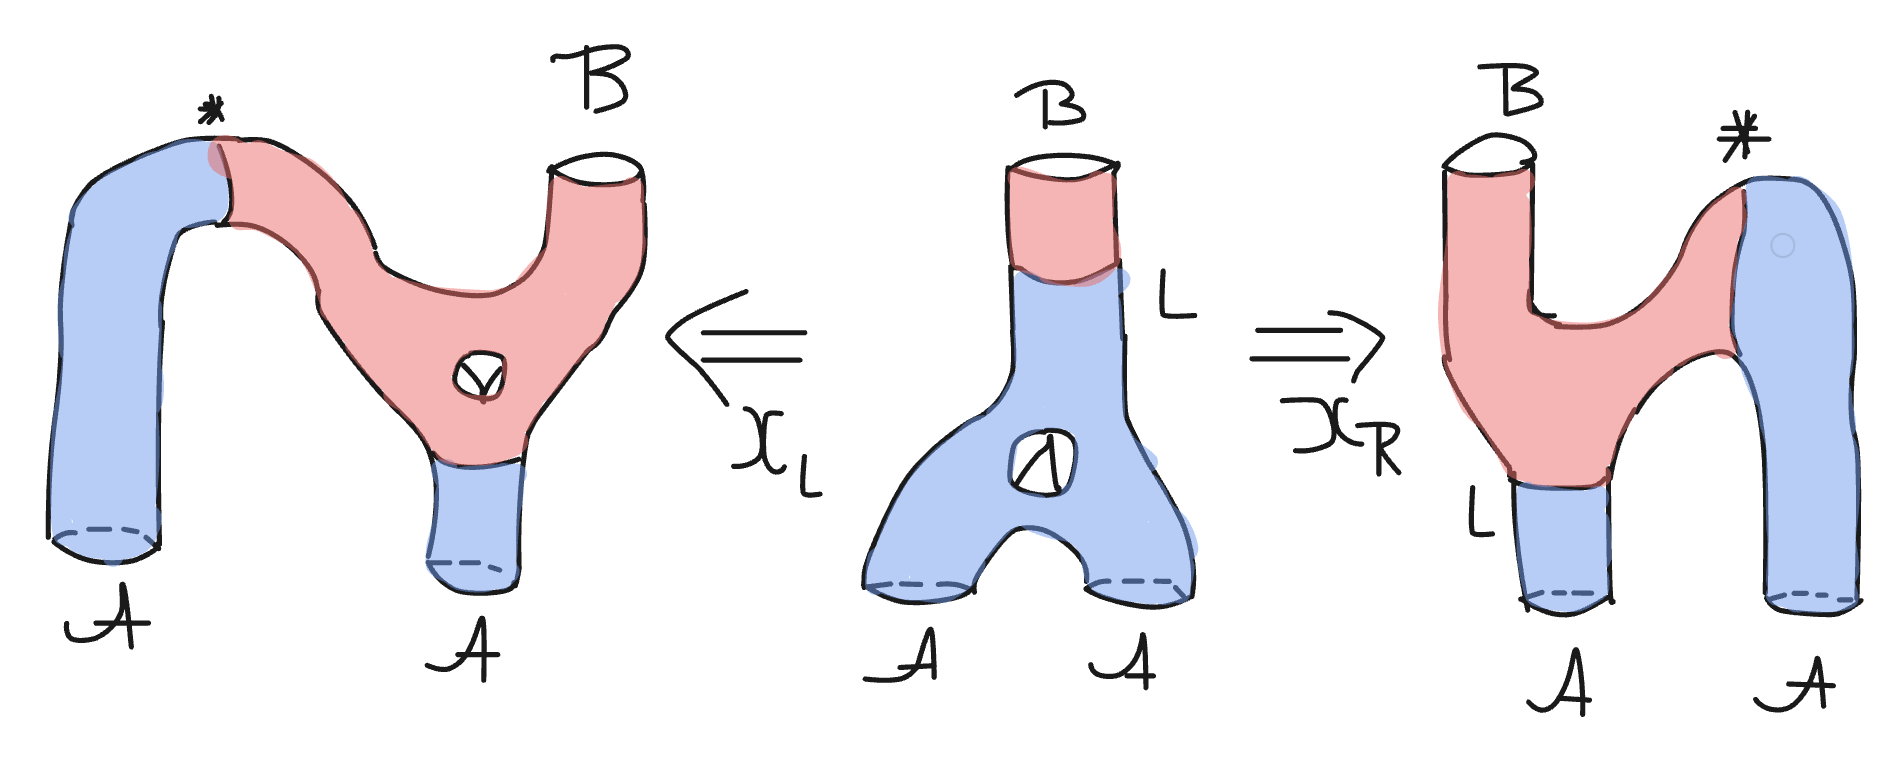
\includegraphics[scale=0.38]{blue-red-28.png}
  \end{center}

  The 1-cell $L : \mathcal{A} \to \mathcal{B}$ is understood as a bracket $\langle a | b \rangle$ between
  $\mathcal{A}$ and $\mathcal{B}$ of the bicategory $\mathcal{V}$. Each side of the above equation may be
  seen as implementing currification set:
  \begin{center}
    $\chi_L : \langle a_1 \circwedge a_2 | b \rangle \Rightarrow \langle a_2 | a^*_1 \circvee b \rangle$

    $\chi_R : \langle a_1 \circwedge a_2 | b \rangle \Rightarrow \langle a_1 | b \circvee a^*_2 \rangle$
  \end{center}
\end{definition}

Every helical dialogue category defines a Frobenius amphimonoid in ${\bf BiMon}$, by taking $La := a \multimap \bot$
and $Ra := \bot \multimapinv a$.

\begin{prop}
  Let $(\mathcal{A}, \mathcal{B})$ be an amphimonoid in a balanced monoidal category $\mathcal{W}$, then
  there is a back-and-forth translation between the following two data:
  \begin{itemize}
    \item the helical Frobenius structures on the pseudomonoids $(\mathcal{A}, \circwedge, true)$,
    \item the Frobenius structures $(L, R, \chi_L, \chi_R)$ on the amphimonoids $(\mathcal{A}, \mathcal{B})$.
  \end{itemize}
\end{prop}

\begin{proof}
  Given an amphimonoid $(\mathcal{A}, \mathcal{B})$, whose $\mathcal{A}$-side is a Frobenius pseudomonoid 
  $(\mathcal{A}, \circwedge, true)$ with Frobenius form noted $||.,.||$, one defines the 1-cells $L$ and $R$ of the
  Frobenius amphimonoid as follows:
  \begin{center}
  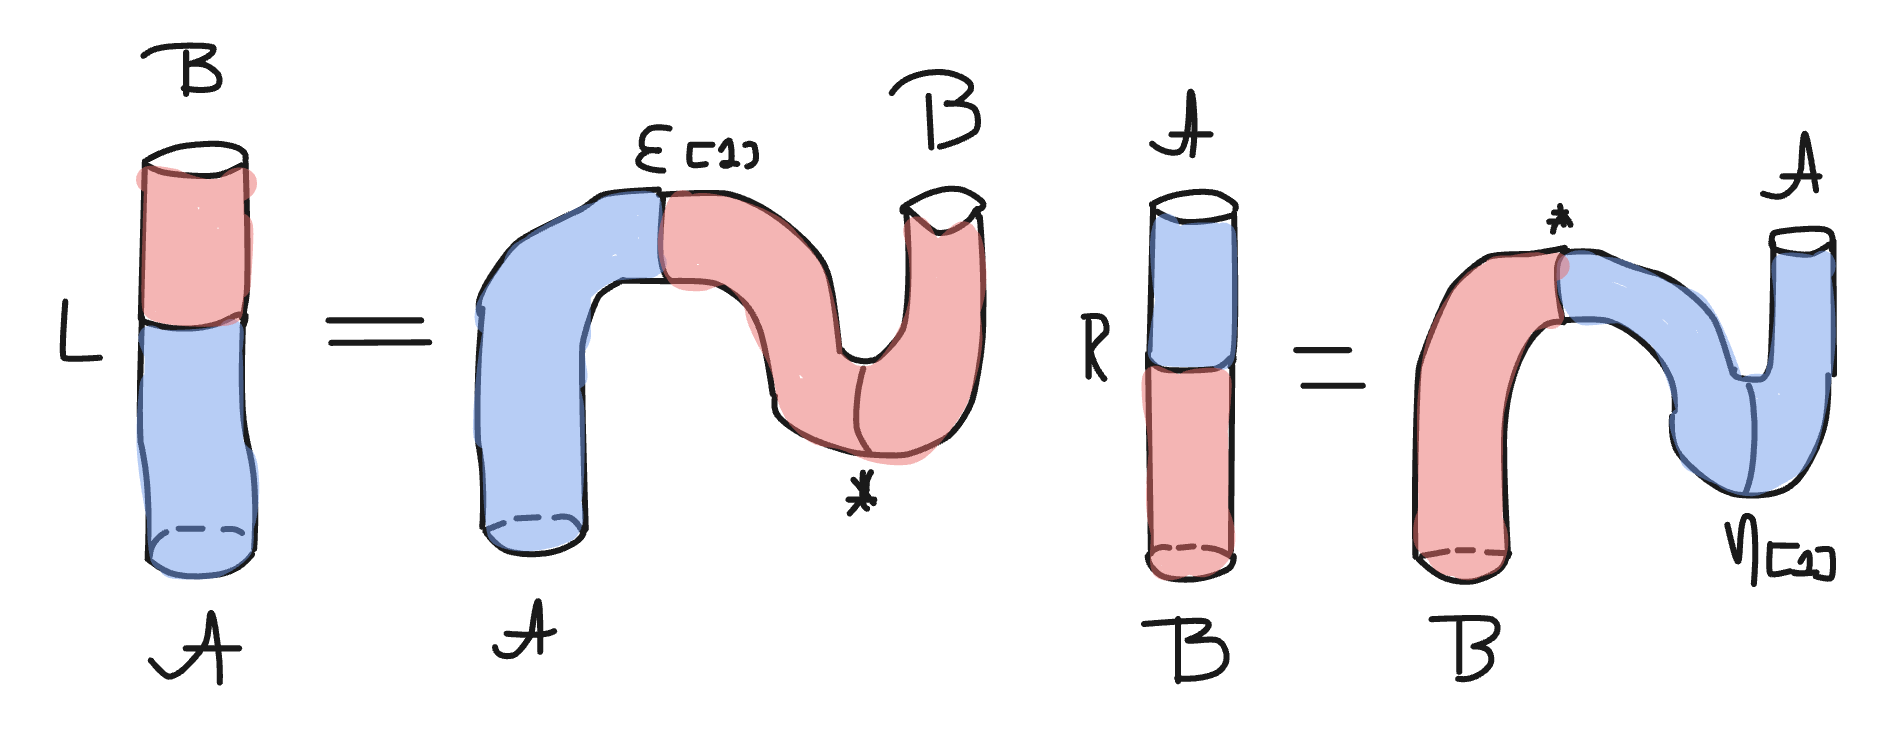
\includegraphics[scale=0.38]{blue-red-29.png}
  \end{center}
  The definition of a lax pairing ensures $L \dashv R$ is indeed an adjunction in $\mathcal{W}$. The 2-cell
  $\chi_R$ is defined as:
  \[
  \begin{tikzcd}
    {||a_1 \circwedge m, a_2||} \ar[rr, Rightarrow, "\chi"] && {||a_1, m \circwedge a_2||}
  \end{tikzcd}
  \]
  whilst $\chi_L$ is given as
  \[
  \begin{tikzcd}
    {||m \circwedge a_1, a_2||} \ar[rr, Rightarrow, "\operatorname{helix}"] && {||a_2, m \circwedge a_1||} \ar[rr, Rightarrow, "\chi^{-1}"] && {||a_2 \circwedge m, a_1||} \ar[rr, Rightarrow, "\operatorname{helix}^{-1}"] && {||a_1, a_2 \circwedge m||}
  \end{tikzcd}
  \]

  Conversely, let $(\mathcal{A}, \mathcal{B}, L, R)$ be a Frobenius amphimonoid in a balanced monoidal
  bicategory $\mathcal{W}$, a Frobenius form is defined the following way on the pseudomonoid $\mathcal{A}$:
  \begin{center}
  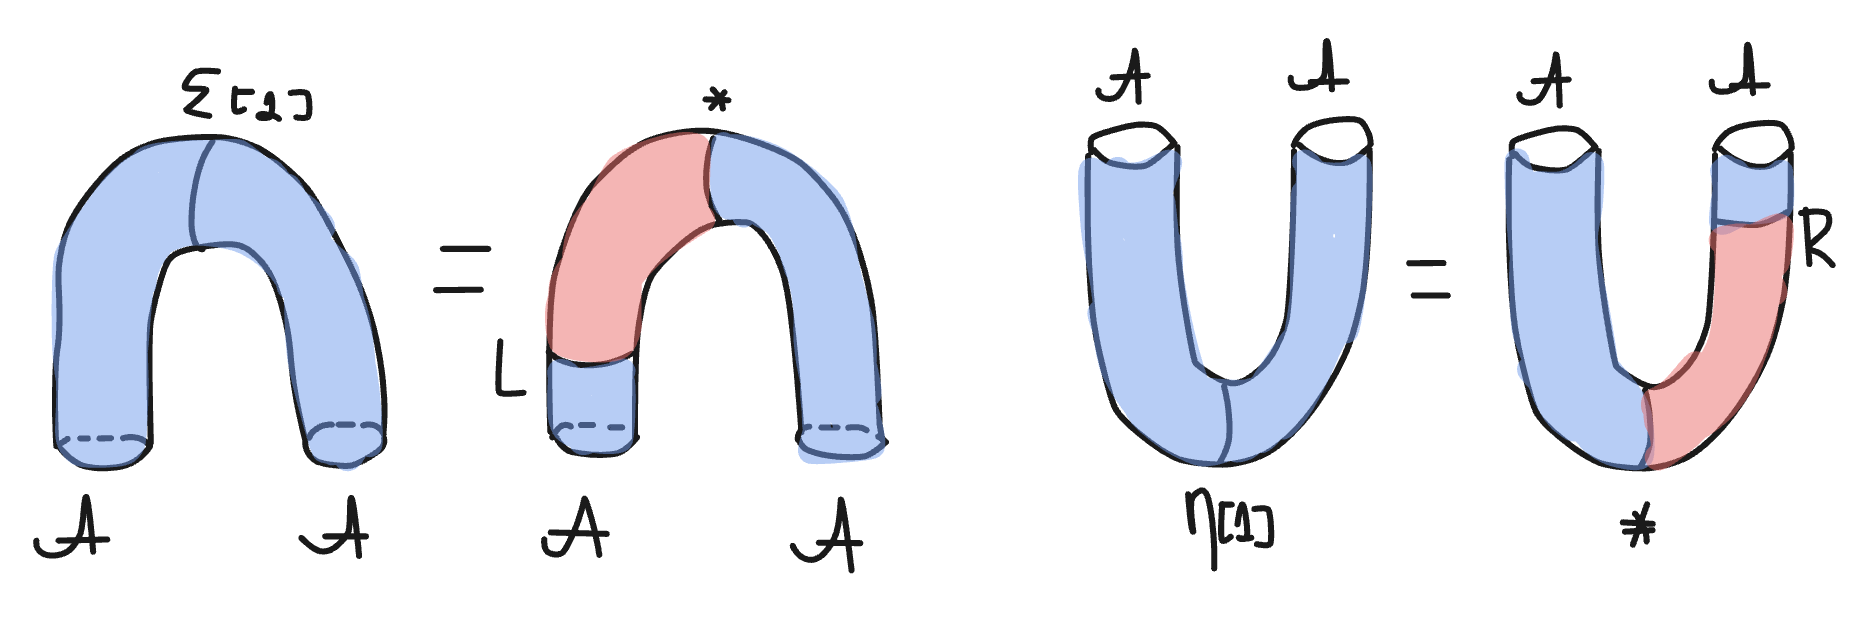
\includegraphics[scale=0.38]{blue-red-30.png}
  \end{center}
  The associativity law $\chi$ of the Frobenius form is defined using $\chi_R$ along with the coercion
  from the definition of a Frobenius amphimonoid and the 2-dimensional structure of the biexact pairing
  $\mathcal{A} \dashv \mathcal{B}$. One obtains a Frobenius pseudomonoid $(\mathcal{A}, \circwedge, true)$,
  whose helical structure is defined using the currification combinators $\chi_L$ and $\chi_R$:
  \begin{center}
  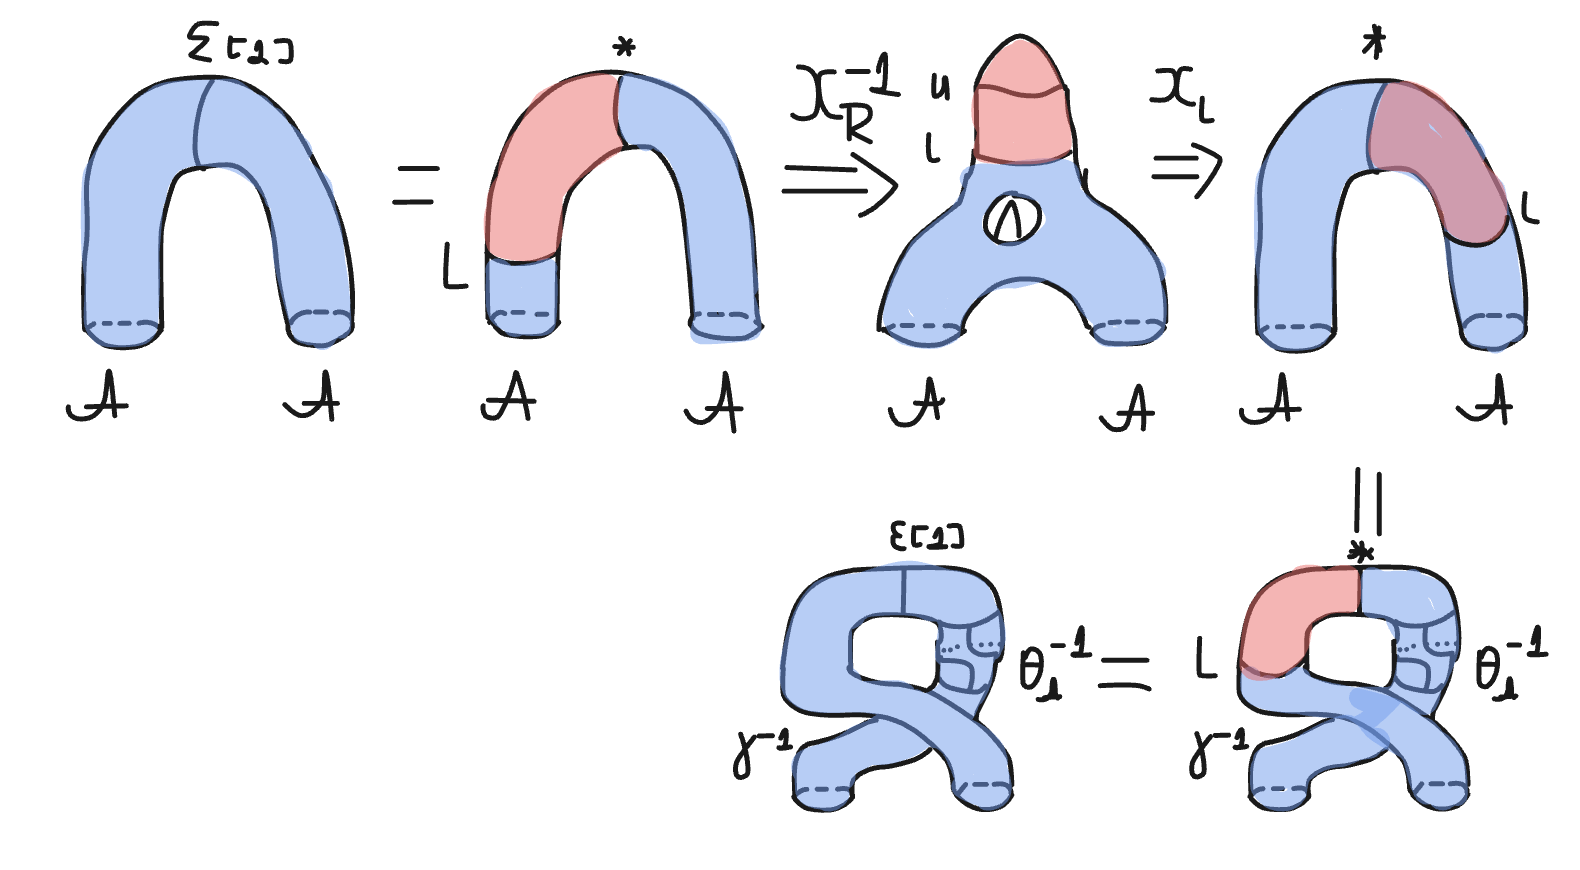
\includegraphics[scale=0.38]{blue-red-31.png}
  \end{center}
\end{proof}

Now let us apply the above proposition to the specific monoidal bicategory ${\bf BiMod}$, where every category
$\mathcal{A}$ comes with the exact pairing $\mathcal{A} \dashv \mathcal{A}^{op}$ whose unit and counit are defined as
the bimodule:
\begin{center}
  $\operatorname{hom} : \mathcal{A}^{op} \times \mathcal{A} \to \operatorname{Set}$

  $\operatorname{hom} : (a_1, a_2) \mapsto \mathcal{A}(a_1, a_2)$
\end{center}

\begin{theorem}{\emph{(First correspondece theorem)}}
  A helical chirality is the same thing as a Frobenius amphimonoid in the bicategory ${\bf BiMod}$
  whose 1-cells
  \begin{center}
  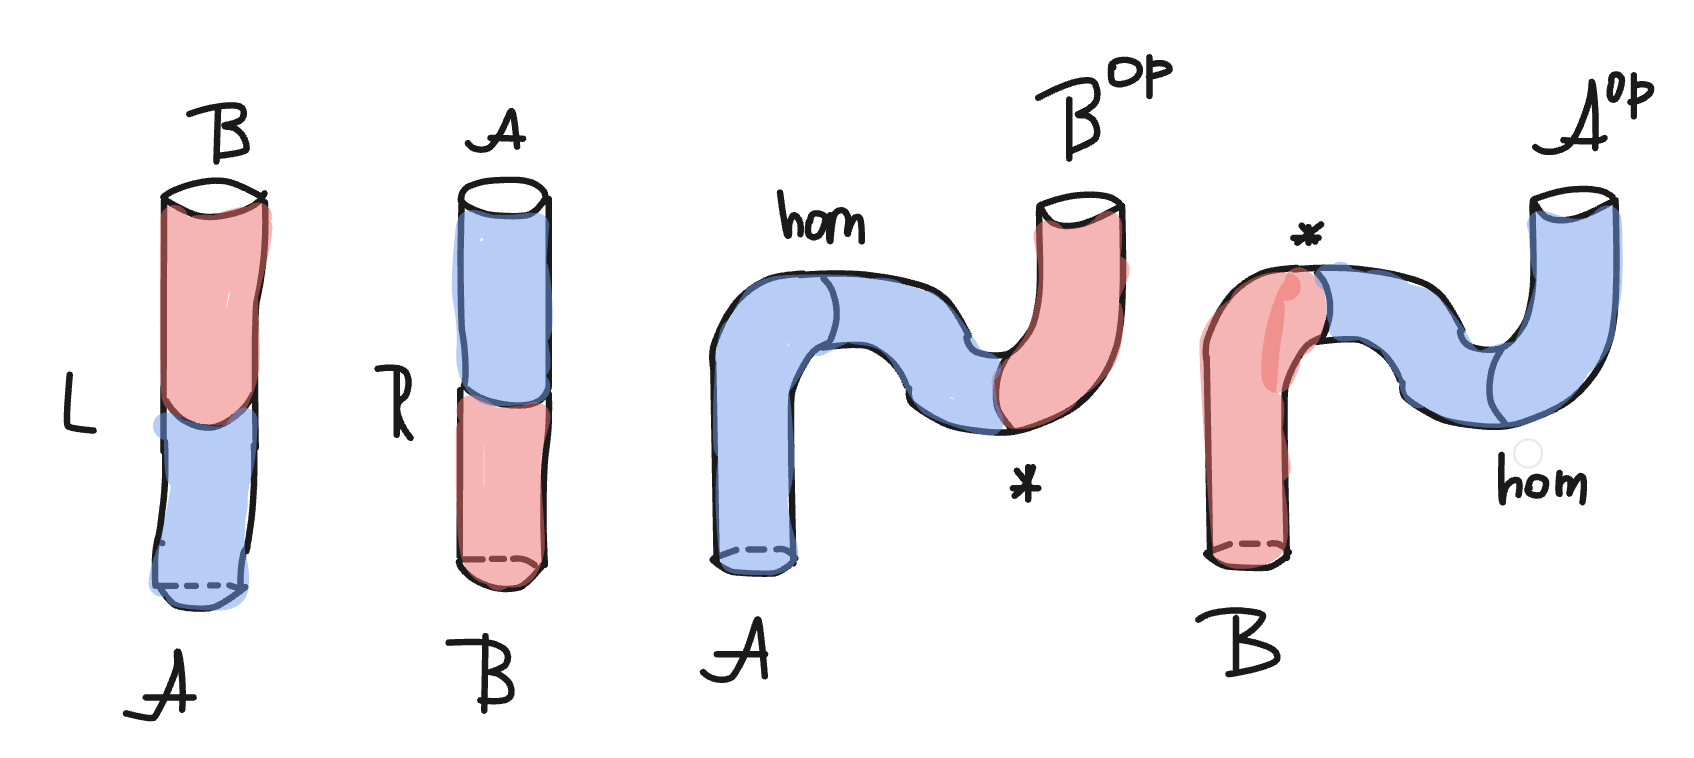
\includegraphics[scale=0.38]{blue-red-32.png}
  \end{center}
  are representable, i.e., images of functors along the 2-dimensional functor $(.)_{\bullet} : {\bf Cat} \to {\bf BiMod}$.
\end{theorem}

\begin{theorem}{\emph{(Second correspondece theorem)}}
  A helical dialogue category is the same thing as a helical Frobenius amphimonoid in the bicategory ${\bf BiMod}$
  whose 1-cells
  \begin{center}
  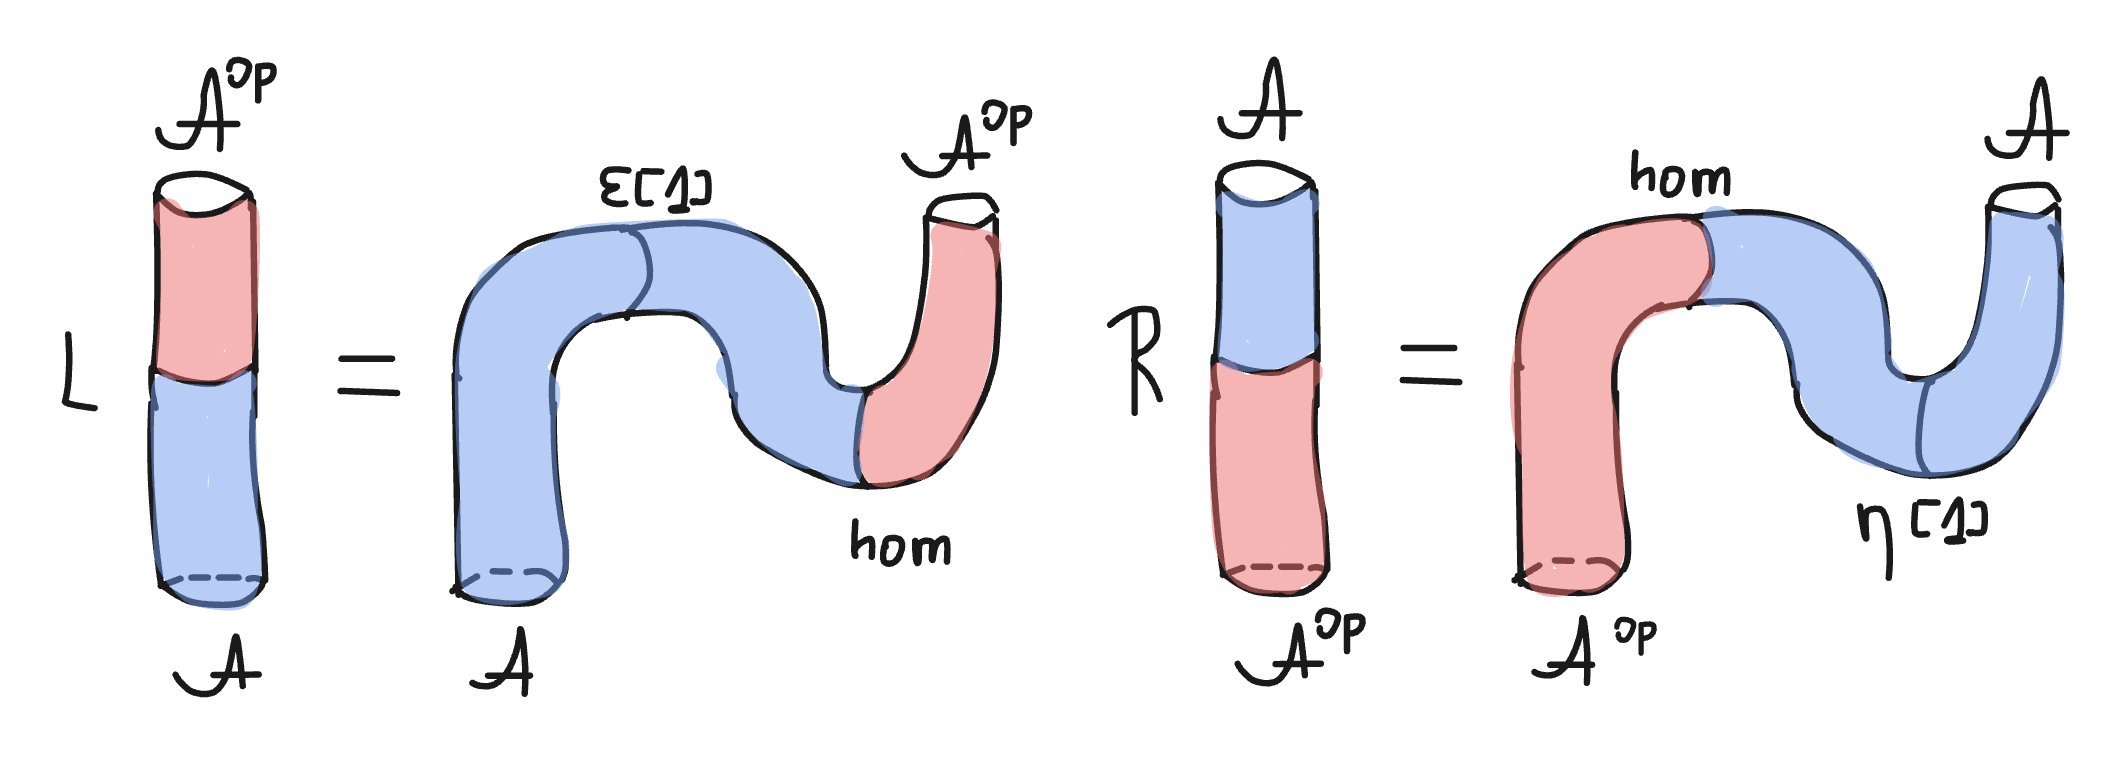
\includegraphics[scale=0.35]{blue-red-33.png}
  \end{center}
  are representable, i.e., images of functors along the 2-dimensional functor $(.)_{\bullet} : {\bf Cat} \to {\bf BiMod}$.
\end{theorem}

\begin{definition}
  A *-autonomous pseudomonoid is a Frobenius pseudomonoid whose Frobenius form is based on the exact pairing $\mathcal{A} \dashv \mathcal{A}$.
\end{definition}

\begin{prop}
  A pseudomonoid $(\mathcal{A}, m, e)$ is Frobenius if and only if it is equipped with 1-cell
  $l : \mathcal{A} \to I$ such that
  \[
  \mathcal{A} \otimes \mathcal{A} \xrightarrow{m} \mathcal{A} \xrightarrow{l} I
  \]
  forms the unit $\eta_{[1]}$ in a lax pairing $\mathcal{A} \dashv \mathcal{A}$.
\end{prop}

\section{Ribbon Tensorial Logic: basic remarks}

Category-theoretically, sequents $A \land A^* \vdash {\bf false}$ and ${\bf true} \vdash A \lor A^*$ define
the following combinators:
\begin{center}
  $\operatorname{cut} : A \land A^* \to {\bf false}$

  $\operatorname{axiom} : {\bf true} \to A \lor A^*$
\end{center}
In the geometry of interaction, those combinators implement input-output channels:
  \begin{center}
  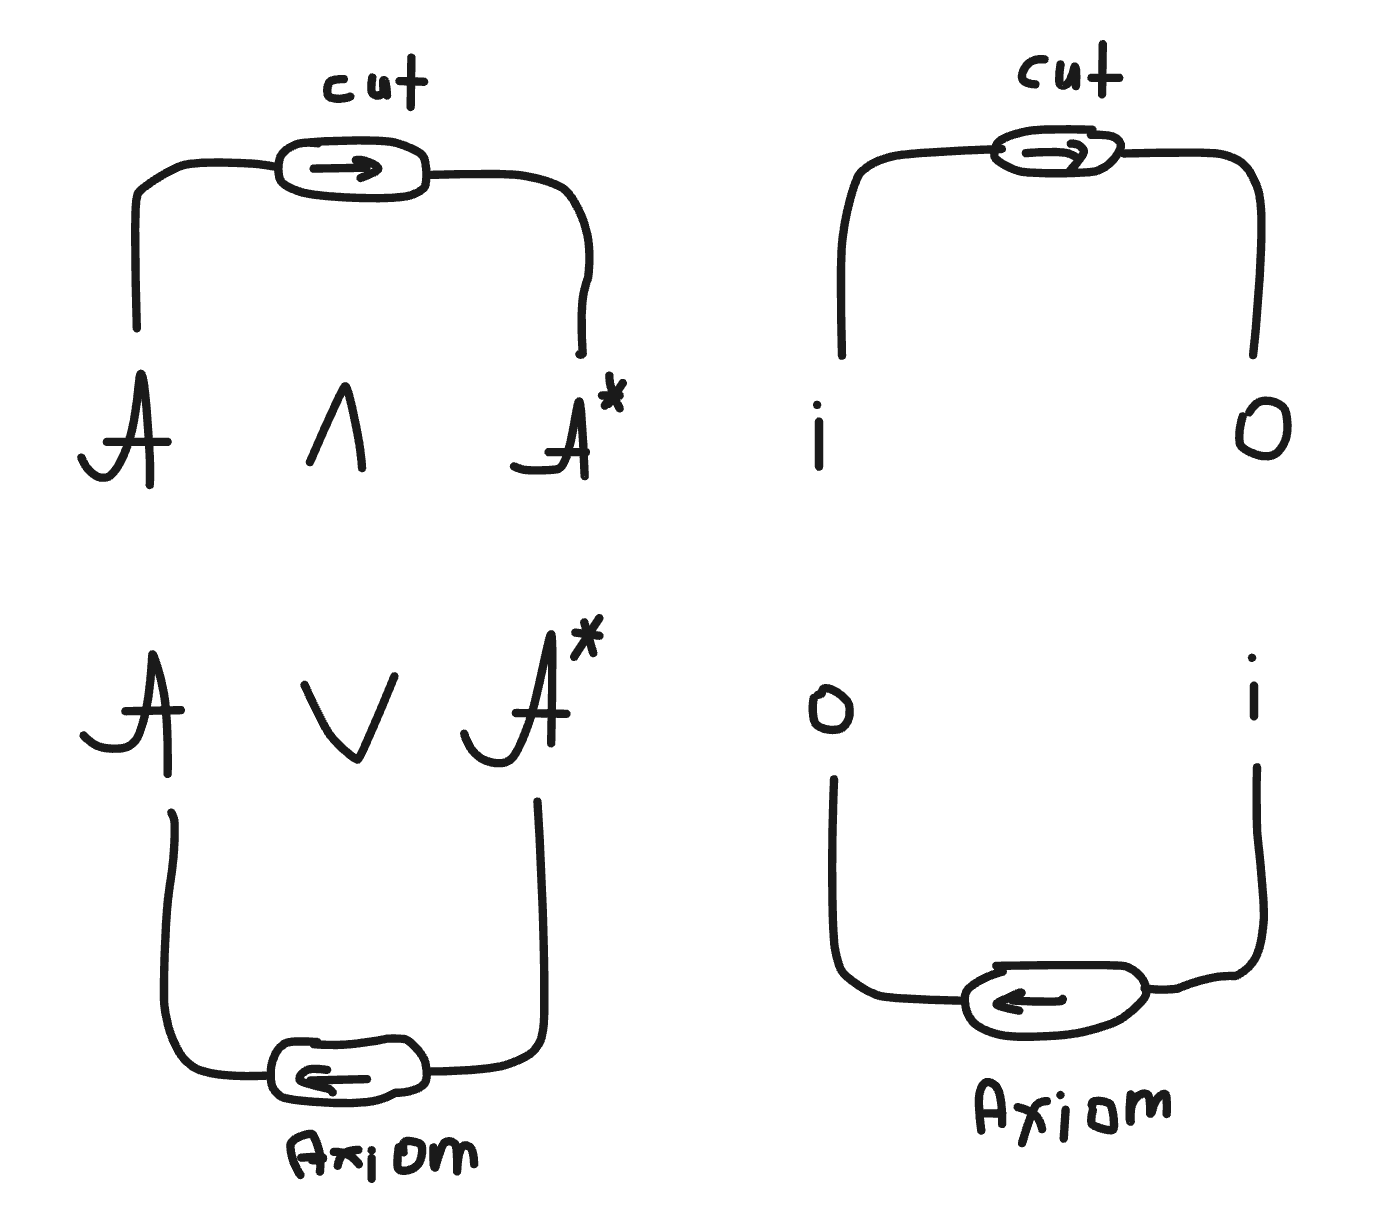
\includegraphics[scale=0.35]{cut-axiom.png}
  \end{center}

In linear logic, one distinguises the notions of \emph{proof structure} and \emph{proof net}. 
In multiplicative linear logic, a proof structure is a proof-like structure using the connectives $\otimes$
and $\parr$ along with the axiom and cut links. A proof tree is a proof structure generated by a derivation tree 
$\pi$. A small example:

  \begin{center}
  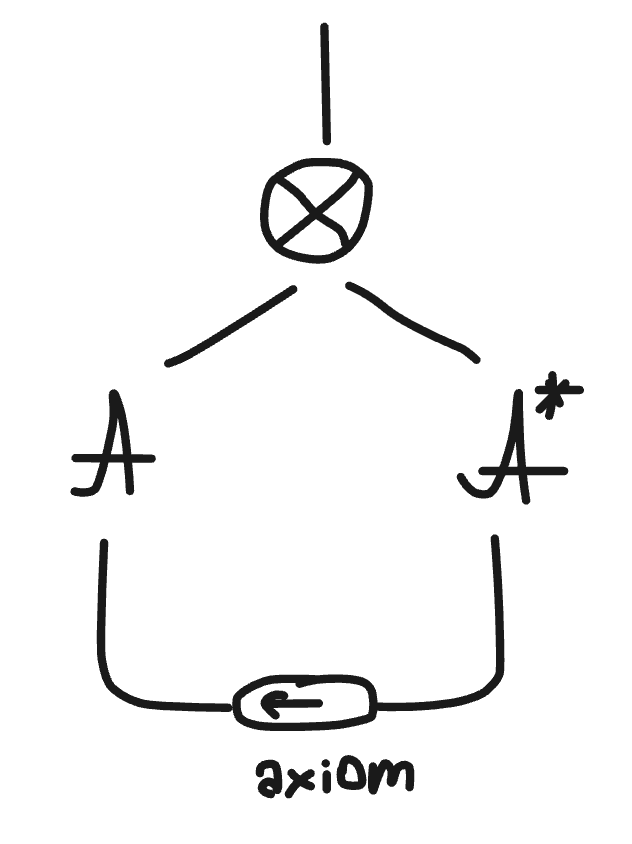
\includegraphics[scale=0.35]{smol-example.png}
  \end{center}

One defines proof nets as specific proof structures generated by generation trees in multiplicative linear logic.
One can also replace the original definition of a proof net with the following one: a multiplicative
proof net is a morphism of the free symmetric *-autonomous category $\operatorname{\bf *-autonomous}(\mathcal{X})$ generated
by a small category $\mathcal{X}$, typically, discrete. One can reformulate the notion of a proof structure
to establish the connections between proof nets and proof structures. 
Recall that a compact closed category is a symmetric monoidal category with unit $I$ where each object $A$
is equipped with an object $A^*$ and a pair of moprhisms 
\begin{center}
  $\operatorname{cut} : A^* \otimes A \to I$

  $\operatorname{axiom} : I \to A^* \otimes A$
\end{center}
such that the following conditions are satisfied:
\[
\begin{tikzcd}
  & A \otimes A^* \otimes A \ar[dr, "A \otimes \operatorname{cut}"] && A^* \ar[dr, "A^* \otimes \operatorname{axiom}"'] \ar[rr, equal] && A^* \\
A \ar[rr, equal] \ar[ur, "\operatorname{axiom} \otimes A"] && A      && A^* \otimes A \otimes A^* \ar[ur, "\operatorname{cut} \otimes A^*"']
\end{tikzcd}
\]
Consider the free compact-closed category $\operatorname{\bf compact-closed}(\mathcal{X})$ for a small category $\mathcal{X}$
for defining proof structures. Those two triangles are visualised the following way in string diagrams:
  \begin{center}
  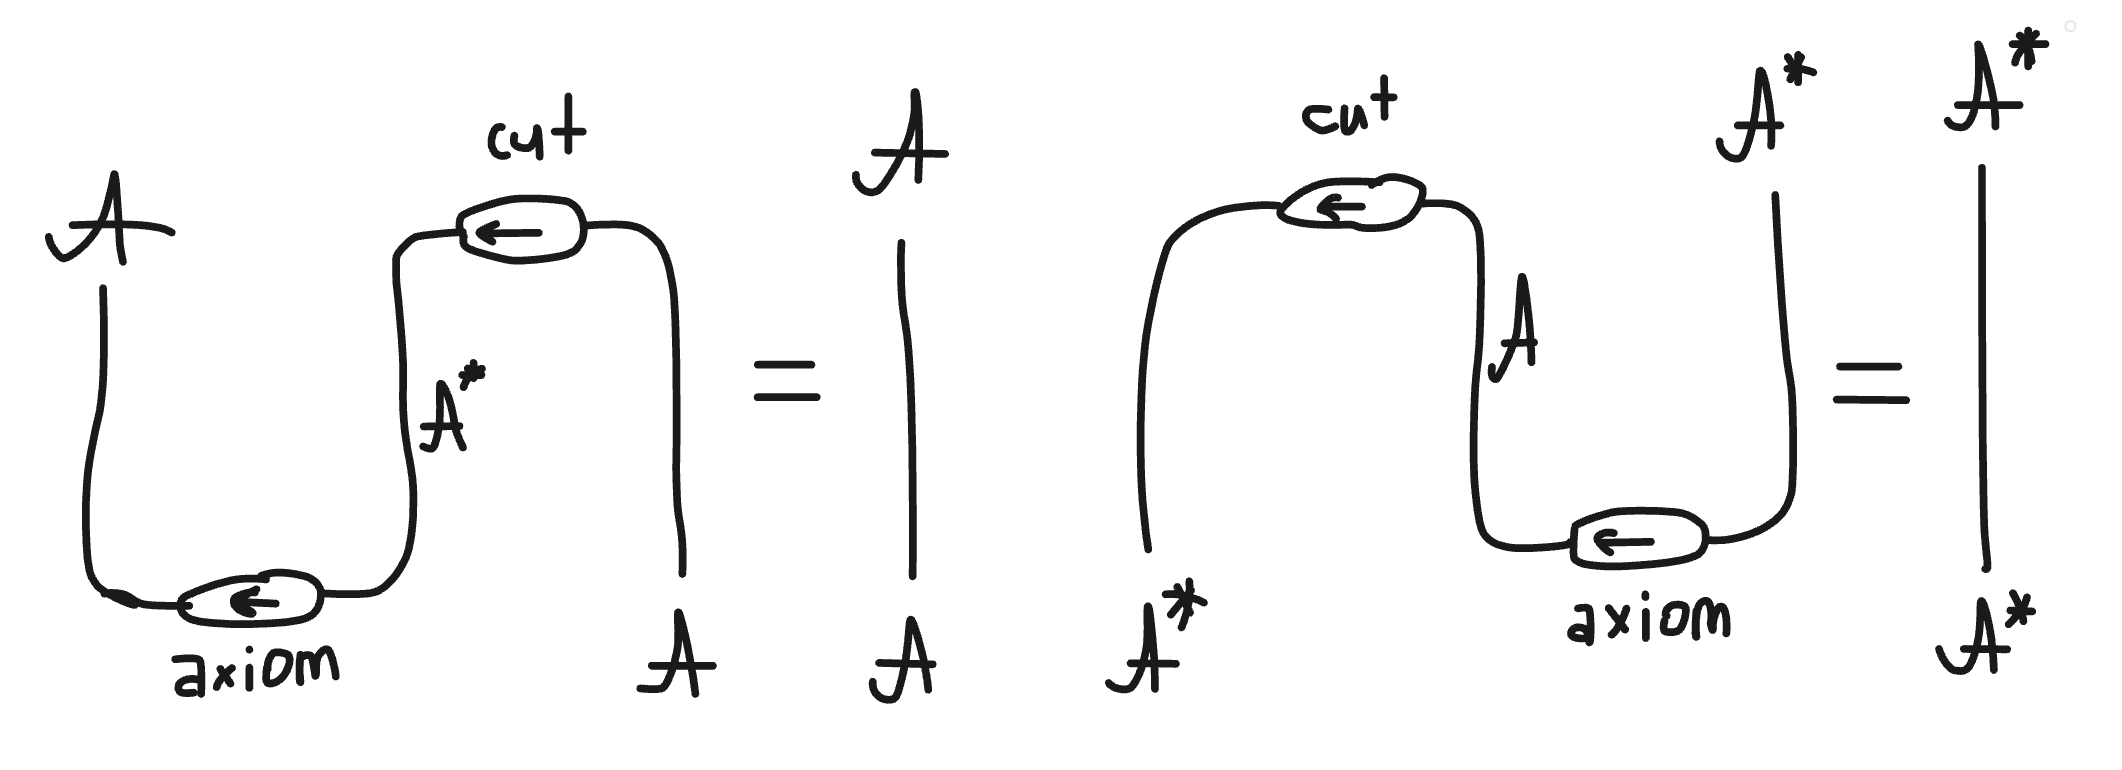
\includegraphics[scale=0.35]{cut-axiom-1.png}
  \end{center}

This makes $A^*$ right dual to $A$, written as $A \dashv A^*$. The operation $A \mapsto A^*$ defines an equivalence
of categories $(.)^* : \mathcal{C}^{op} \to \mathcal{C}$. In other words, a compact-closed category is a *-autonomous category
where $\otimes$ and its opposite $\parr$ coincide up to symmetric monoidal equivalence.

The construction of the free compact closed category generated by $\mathcal{X}$ comes with a functor 
$\mathcal{X} \to \operatorname{\bf compact-closed}(\mathcal{X})$. This functor can be lifted to the structure preserving functor between
*-autonomous categories:
\[
[.] : \operatorname{\bf *-autonomous}(\mathcal{X}) \to \operatorname{\bf compact-closed}(\mathcal{X})
\]
such that the following triangle commutes:
\[
\begin{tikzcd}
  \operatorname{\bf *-autonomous(\mathcal{X})} \ar[rr, "{[}.{]}"] && \operatorname{\bf compact-closed}(\mathcal{X}) \\
  & \mathcal{X} \ar[ur, "atoms"'] \ar[ul, "atoms"]
\end{tikzcd}
\]

Thus, we have a categorical definition of a proof structure:

\begin{definition}
  Let $A$ and $B$ be formulas of multiplicative linear logic with objects from $\mathcal{X}$
  as atoms, a \emph{proof structure} from $A$ to $B$ is a morphism $\Theta : [A] \to [B]$ in 
  the free compact-closed category generated by $\mathcal{X}$. A proof structure for a formula $A$ is a proof structure
  $\Theta : I \to [A]$.
\end{definition}

Let us consider an example for the discrete category with a single element $\alpha$. The functor $[.]$ 
applied to a formula $A$ replaces each occurence of $\otimes$ and $\parr$ with a tensor product. Therefore, $A \otimes A^*$
and $A \parr A^*$ are interpreted the same way:
\[
[A \otimes A^*] = \alpha \otimes \alpha^* = [A \parr A^*]
\]
By the definition, the morphism $\operatorname{axiom} : I \to \alpha \otimes \alpha^*$ of the category 
$\operatorname{\bf compact-closed}(\mathcal{X})$ is depicted as:
  \begin{center}
  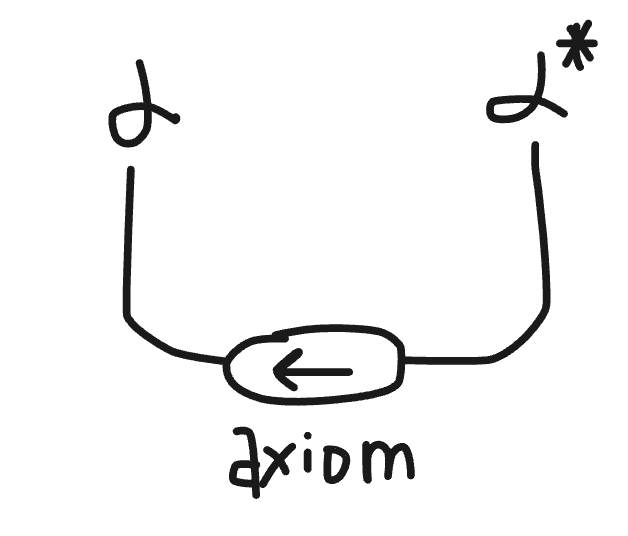
\includegraphics[scale=0.35]{alpha-morphism.png}
  \end{center}
defines a proof structure $\theta$ of the formula $\alpha \otimes \alpha^*$ as well as a proof structure $\theta'$ of the formula 
$\alpha \parr \alpha^*$. The difference is that $\theta'$ is the image of a proof net $\pi : 1 \to \alpha \otimes \alpha^*$
\[
\theta' = [\pi] : I \to [\alpha \otimes \alpha^*],
\]
whereas $\theta$ is not.

There is a limitation that proof structures generally do not characterise proof nets 1 by 1. The analogous situation 
is that the identity and symmetry morphisms
\[
{\bf id}, {\bf symm} : \bot \otimes \bot \to \bot \otimes \bot
\]
generally do not have to coincide in *-autonomous categories. Consider the following derivation trees:
\begin{prooftree}
  \AxiomC{$ $}
  \RightLabel{\bf ax}
  \UnaryInfC{$\vdash 1, \bot$}
  \AxiomC{$ $}
  \RightLabel{\bf ax}
  \UnaryInfC{$\vdash 1, \bot$}
  \RightLabel{$\otimes$}
  \BinaryInfC{$\vdash 1, 1, \bot \otimes \bot$}
  \RightLabel{$\parr$}
  \UnaryInfC{$\vdash 1 \parr 1, \bot \otimes \bot$}
\end{prooftree}
\begin{prooftree}
  \AxiomC{$ $}
  \RightLabel{\bf ax}
  \UnaryInfC{$\vdash 1, \bot$}
  \AxiomC{$ $}
  \RightLabel{\bf ax}
  \UnaryInfC{$\vdash 1, \bot$}
  \RightLabel{$\otimes$}
  \BinaryInfC{$\vdash 1, 1, \bot \otimes \bot$}
  \RightLabel{\bf exch}
  \UnaryInfC{$\vdash 1, 1, \bot \otimes \bot$}
  \RightLabel{$\parr$}
  \UnaryInfC{$\vdash 1 \parr 1, \bot \otimes \bot$}
\end{prooftree}
Those tree are different only in applying the exchange rule in the second one, but they also define different morphisms
in the free *-autonomous category, and therefore different proof nets $\pi_1$ and $\pi_2$. But their images $[\pi_1]$ and $[\pi_2]$
in the free compact closed category coincide since $I = [1] = [\bot]$, and the following morphisms
\[
{\bf id}, {\bf symm} : I \otimes I \to I \otimes I
\]
coincide in every symmetric monoidal category. Therefore, some information from the proofs nets $\pi_1$ and $\pi_2$
was lost after the translation. In more generic terms, this restriction can be formulated completely categorically is that the
canonical functor $[.] : \operatorname{\bf *-autonomous}(\mathcal{X}) \to \operatorname{\bf compact-closed}(\mathcal{X})$ is not faithful.

One can improve this restriction by taking a more general formalism than linear logic, tensorial logic,
where negation is not involutive. To proceed further, one needs to take some ideas from knot theory and representation theory.
The aim is to materialise links $[\pi]$ of a proof $\pi$. 

The concept of a ribbon category is equipped with a coherence theorem, stating that the free ribbon category ${\bf ribbon}(\mathcal{X})$ has
\begin{itemize}
  \item Objects: sequences $(A^{\epsilon_1}_1, \ldots, A^{\epsilon_n}_n)$ of signed objects of $\mathcal{X}$ where each $\epsilon_i$ is either $+$ or $-$.
  \item Morphisms: oriented ribbon tangles modulo topological deformation, where every open strand is coloured
  by a morphism of $\mathcal{X}$, and every closed strand is coloured by an equivalence class of morphisms modulo
  $f \circ g \sim g \circ f$ for a pair of morphisms $f : A \to B$ and $g : B \to A$.
\end{itemize}
For example, a morphism from $(A^+)$ to $(B^+, C^-, D^+)$ in ${\bf ribbon}(\mathcal{X})$ looks like this:
  \begin{center}
  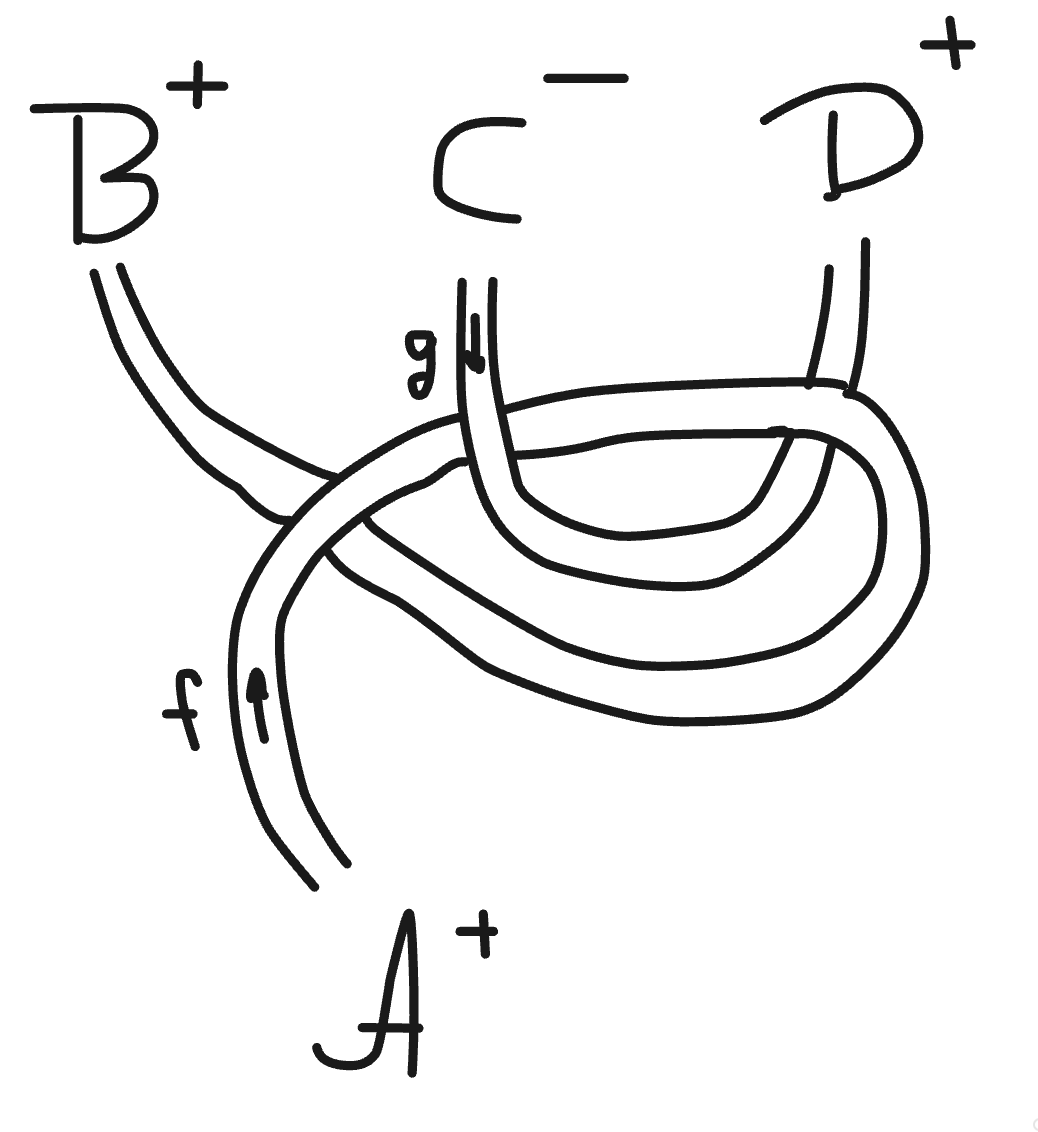
\includegraphics[scale=0.25]{ribbon-morphism.png}
  \end{center}
for $f : A \to B$ and $g : C \to D$ in $\mathcal{X}$.

Now consider the full and faithful functor $\mathcal{X} \to {\bf ribbon}(\mathcal{X})$ transporting every
object $A$ to the one-element sequence $(A^+)$. Every functor from the category $\mathcal{X}$ to a ribbon category $\mathcal{D}$
lifts as a structure-preserving $\langle . \rangle$ (this is the universal property of the free algebras):
\[
\begin{tikzcd}
  {\bf ribbon}(\mathcal{X}) \ar[rr, "\langle . \rangle"] && \mathcal{D} \\
  & \mathcal{X} \ar[ul, "\operatorname{links}"] \ar[ur, "\operatorname{interpretation \: of \: links}"']
\end{tikzcd}
\]

Every topological ribbon knot defines a morphism $P : I \to I$, so its image $\langle P \rangle$ defines an invariant
of a knot $P$ modulo topological deformation. For instance, the functorial method allows establishing that the Jones
polynomial $\langle P \rangle$ associated to a ribbon invariant. For example, the left trefoil $K_L$ and the right trefoil
$K_R$
  \begin{center}
  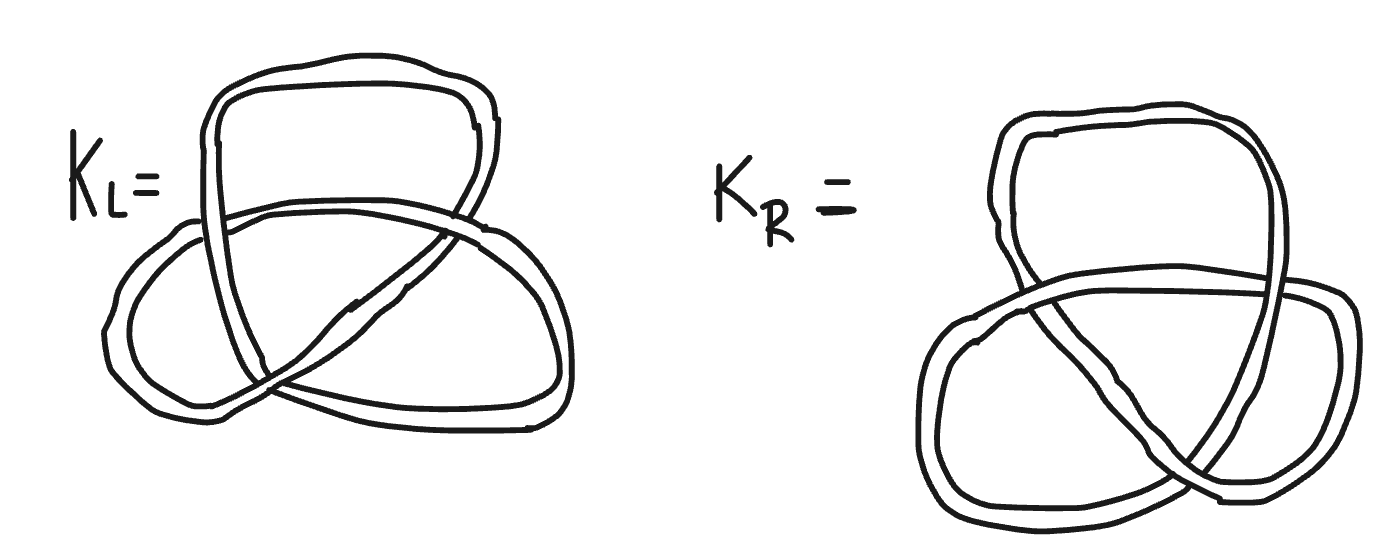
\includegraphics[scale=0.28]{trefoils.png}
  \end{center}
are different modulo knot deformation as their Jones polynomials are different:
\[\langle K_L \rangle = \frac{2}{x^2} + \frac{1}{x^4} + \frac{y^2}{x^2}
\]
\[\langle K_R \rangle = 2x^2 - x^4 + x^2 y^2
\]

The braided concept of a dialogue category allows connecting proof theory and knot theory, so we will be working
with balanced dialogue categories and ribbon tensorial logic. One has a similar coherence theorem from balanced dialogue categories and ribbon tensorial logic
claiming that the free balance dialogue category generated by a category $\mathcal{X}$ has:
\begin{itemize}
  \item objects: formulas of ribbon tensorial logic with atoms provided by the objects of $\mathcal{X}$,
  \item morphisms: the derivation trees $\pi$ of proofs $A \vdash B$ factorised module the corresponding equational theory.
\end{itemize}

Now let us have a glance at the proof-as-tangle theorem closer. The next is to equip balanced dialogue categories
with a topological content. 

A pointed category $(\mathcal{C}, \bot)$ is a category with a distinguished object $\bot \in \mathcal{C}$.
Alternatively, one can think of a pointed category as an $S$-algebra for the monad $S : {\bf Cat} \to {\bf Cat}$
sending each category $\mathcal{C}$ to $\mathcal{C} \sqcup {\bf 1}$, where ${\bf 1}$ is the terminal category.
The unique object $\bot$ of ${\bf 1}$ provides the single-out object of the pointed category $(\mathcal{C} \sqcup {\bf 1}, \bot)$.
Every category $\mathcal{C}$ induces a free ribbon category ${\bf ribbon}(\mathcal{C} \sqcup {\bf 1})$
generated by $\mathcal{C} \sqcup {\bf 1}$. By the construction,  ${\bf ribbon}(\mathcal{C} \sqcup {\bf 1})$ is monoidal and balanced.
${\bf ribbon}(\mathcal{C} \sqcup {\bf 1})$ is also dialogue as the negations are given by:
\begin{center}
  $x \multimap \bot := x^* \otimes \bot$

  $\bot \multimapinv x := \bot \otimes x^*$
\end{center}
Note that, the following canonical morphism defining the strength of the double negation monad
\[
(\bot \multimapinv (x \multimap \bot)) \otimes y \to \bot \multimapinv ((x \otimes y) \multimap \bot)
\]
is an isomorphism in the resulting balanced dialogue category.

The unit of the monad $S$ instantiated for $\mathcal{C}$
\[
{\bf return}_{\mathcal{C}} : \mathcal{C} \to \mathcal{C} \sqcup {\bf 1}
\]
induces the following functor:
\[
\mathcal{C} \to \mathcal{C} \sqcup {\bf 1} \to {\bf ribbon}(\mathcal{C} \sqcup {\bf 1})
\]
Therefore, there is a structure-preserving functor of balanced dialogue categories:
\[
[.] : \operatorname{\bf balanced-dialogue}(\mathcal{C}) \to {\bf ribbon}(\mathcal{C} \sqcup {\bf 1})
\]
such that the following square commutes:
\[
\begin{tikzcd}
  \mathcal{C} \ar[dd] \ar[rr, "{\bf return}_{\mathcal{C}}"] && \mathcal{C} \sqcup {\bf 1} \ar[dd] \\
  \\
  \operatorname{\bf balanced-dialogue}(\mathcal{C}) \ar[rr, "{[}.{]}"'] && {\bf ribbon}(\mathcal{C} \sqcup {\bf 1})
\end{tikzcd}
\]
The functor $[.]$ transports:
\begin{itemize}
  \item formulas of ribbon tensorial logic into signed sequences of $\bot$'s and logical atoms provided by 
  the objects of $\mathcal{C}$,
  \item proofs modulo the equational theory into ribbon tangles modulo topological deformation.
\end{itemize}

\begin{definition} A tensorial proof net $\pi$ of ribbon tensorial logic is a morphism in a free balanced dialogue category.
\end{definition}

\begin{definition}
  A tensorial proof structure of ribbon tensorial logic from a formula $A$ to a formula $B$ is a morphism 
  $\Theta : [A] \to [B]$ is a free ribbon category.
\end{definition}

\begin{theorem}
  The canonical functor
  \[
  [.] : \operatorname{\bf symmetric-dialogue}(\mathcal{C}) \to \operatorname{\bf compact-closed}(\mathcal{C} \sqcup {\bf 1})
  \]
  transporting tensorial proof nets to tensorial proof structures in commutative tensorial logic, is faithful.
\end{theorem}

The theorem effectively means that in ribbon tensorial logic (as well as in commutative linear logic),
derivation trees $\pi$ are entirely characterised by their proof structures $[\pi]$. This theorem also connects
proof theory with knot theory by providing a topological coherence theorem.

\section{On Balanced Dialogue Categories and Ribbon Tensorial Logic}

Recall that in balanced categories, the twist $\theta_A$ is visualised as the ribbon $A$ twisted positively in
the trigonometric direction with an angle $2\pi$, whereas its inverse $\theta^{-1}_A$ is depicted the same way
as $A$, but twisted negatively with an angle $-2\pi$:
  \begin{center}
  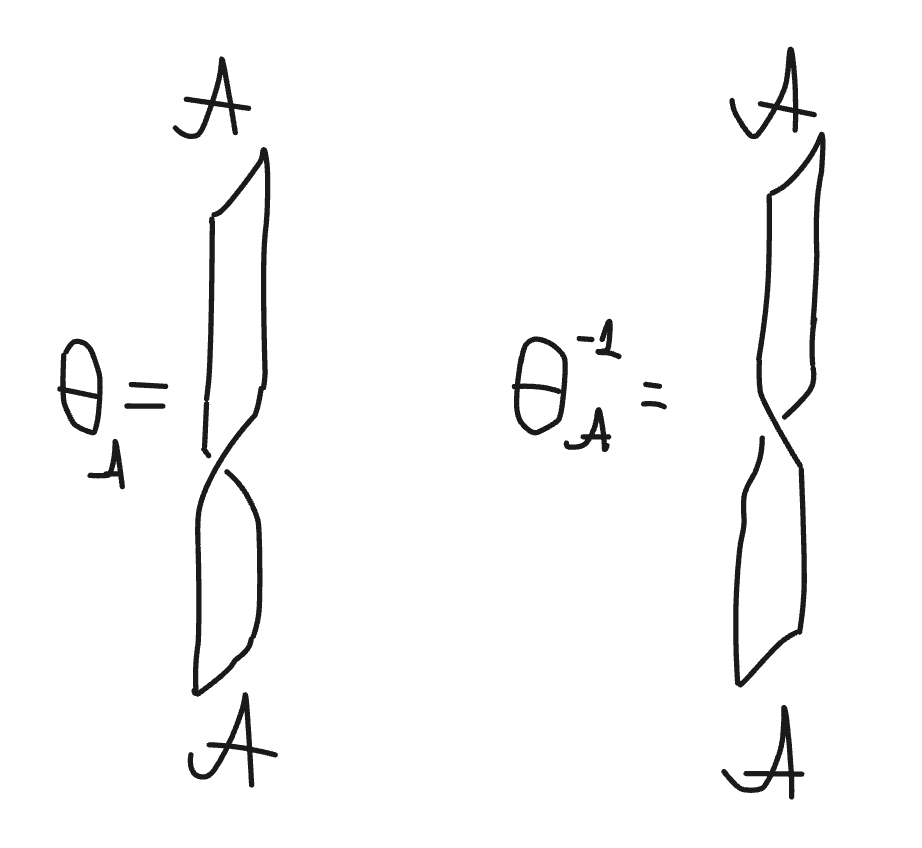
\includegraphics[scale=0.25]{twisted-ribbons.png}
  \end{center}
So one can reword the commutative square from the definition of a balanced category is visualised as follows:
  \begin{center}
  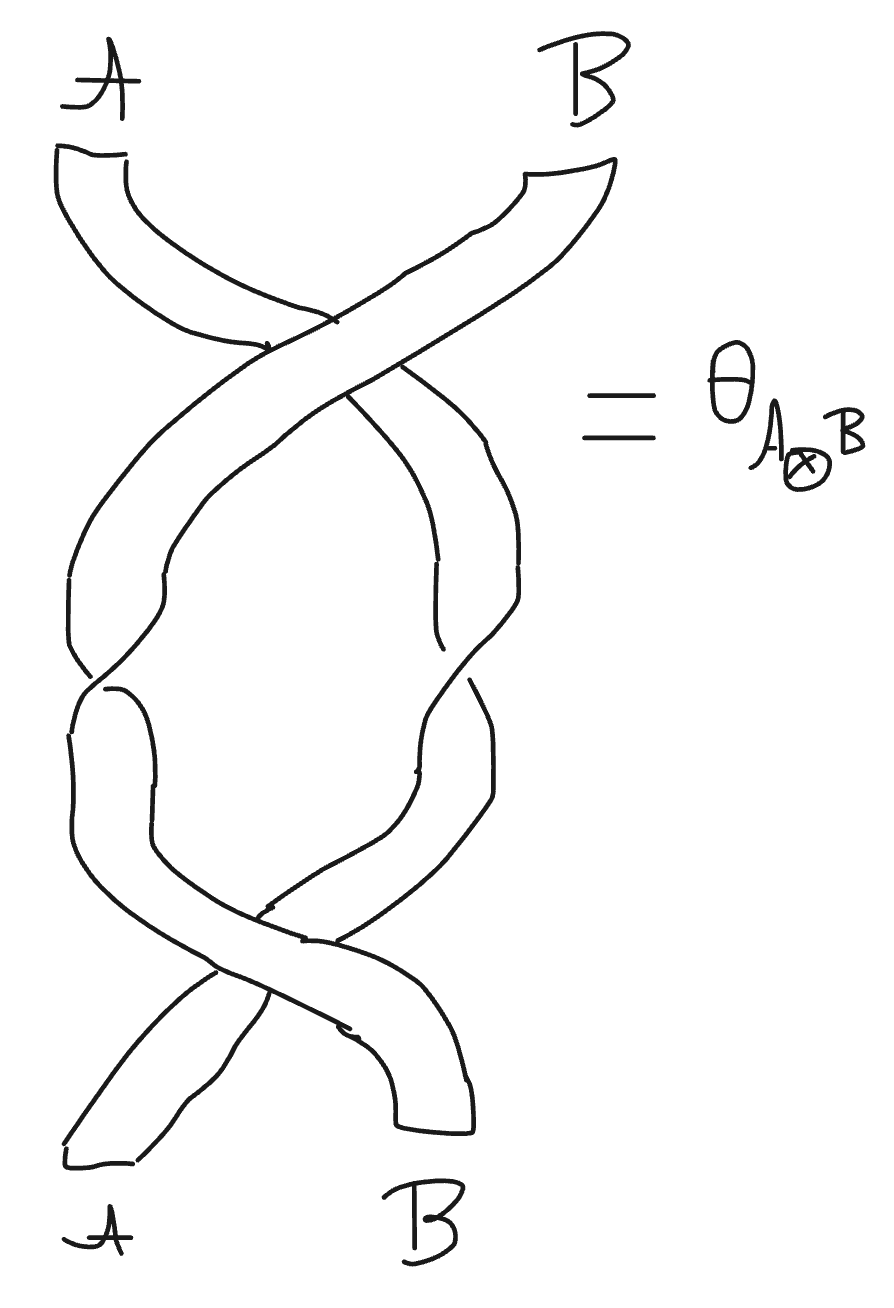
\includegraphics[scale=0.25]{twisted-ribbons-2.png}
  \end{center}


\begin{definition}
  A \emph{balanced dialogue category} is a dialogue category equipped with twists and braiding.
\end{definition}

One can extract an example of a balanced monoidal category from algebra, in particular, from the representation of quantum groups.
The category ${\bf Mod}(H)$ of (finite or infinite dimensional) $H$-modules associated to a ribbon Hopf algebra $H$.
The full subcategory of rigid objects (i.e., those ones that have a right dual) in ${\bf Mod}(H)$ (or in any other balanced 
dialogue category) is a ribbon category. Typically, the category ${\bf Mod}_f(H)$ of finite dimensional
$H$-modules associated to a ribbon Hopf algebra $H$ defines a ribbon category.

Recall that the braid group ${\bf B}_n$ on $n < \omega$ strands is presented by generators $\{ \sigma_i \: | \: 1 \leq i \leq n - 1 \}$
and the following equations:
\begin{center}
  $\sigma_i \circ \sigma_{i + 1} \circ \sigma_i = \sigma_{i + 1} \circ \sigma_i \circ \sigma_{i + 1}$

  $\sigma_i \circ \sigma_j = \sigma_j \circ \sigma_i$ for either $|j - i| \leq 2$
\end{center}

There is a left action:
\[
\triangleleft : {\bf B}_n \times [n] \to [n]
\]
of the group ${\bf B}_n$ to the set $[n] = \{ 1, \ldots, n \}$ of strands induced by the group homomorphisms
${\bf B}_n \to {\bf S}_n$, where ${\bf S}_n$ is the symmetry group on $n$ elements.
This action defines a wreath product of ${\bf B}_n$ on the additive group $(\mathbb{Z}, +, 0)$.
The resulting group is ${\bf G}_n$, the ribbon group on $n$ strands. It is defined on the generates 
$\{ \sigma_i \: | \: 1 \leq i \leq n - 1 \}$ and $\{ \theta_i \: | : 1 \leq i \leq n \}$ and the related from the definition of a braid group
along with the following ones:
\begin{itemize}
  \item $\sigma_i \circ \theta_i = \theta_{i + 1} \circ \sigma_i$,
  \item $\sigma_i \circ \theta_{i + 1} = \theta_i \circ \sigma_i$,
  \item $\sigma_i \circ \theta_j = \theta_j \circ \sigma_i$ for either $j < i$ or $j \geq i + 2$.
\end{itemize}

One can conceptually rephrase ribbon groups as follows. The groupoid $\mathcal{G}$ defined as the disjoint sum of groupoids
$S {\bf G}_n$ coincides with the free balanced category generated by the terminal category ${\bf 1}$. The group
${\bf G}_n$ can be alternatively defined as $\mathcal{G}(n,n)$ where
\[
n = 1 \otimes \ldots \otimes 1
\]
is the $n$-fold tensor product of the generator $1$ in the terminal category ${\bf 1}$. Therefore, we have a family of group homomorphisms
\[
\otimes : {\bf G}_p \times {\bf G}_q \to {\bf G}_{p + q}
\]
reflecting the monoidal structure of the balanced category $\mathcal{G}$. Moreover, the above defined action
\[
\triangleleft : {\bf G}_n \times [n] \to [n]
\]
where each $\theta_i$ acts trivially $[n] = \{ 1, \ldots, n \}$ in the sense that $\theta_i \triangleleft k = k$
for each $k \in [n]$.

\section{The Sequent Calculus and its commuting conversions}

The formulas of ribbon tensorial logic is generated by the following grammar:
\[
A, B ::= {\bf 1} \: | \: \alpha \: | \: \bot \: | \: (A \otimes B) \: | \: (A \multimap \bot) \: | \: (\bot \multimapinv A)
\]
where $\alpha$ ranges over objects from a small category $\mathcal{X}$.

The sequents have the form of:
\[
A_1, \ldots, A_m \vdash B
\] 
where $A_1, \ldots, A_m$ is a sequence of formula and $B$ is a single formula. The inference rules are given in Figure~\ref{fig:1}.

\begin{figure}[H]
  \hrule
  \caption{Ribbon Tensorial Logic}~\label{fig:1}
  \begin{minipage}{0.5\textwidth}
    \begin{prooftree}
      \AxiomC{$f : A \to B \in \mathcal{X}$}
      \RightLabel{${\bf ax}$}
      \UnaryInfC{$A \vdash B$}
    \end{prooftree}

    \begin{prooftree}
      \AxiomC{$\Gamma_1, \Gamma_2 \vdash A$}
      \RightLabel{${\bf 1}_L$}
      \UnaryInfC{$\Gamma_1, {\bf 1}, \Gamma_2 \vdash A$}
    \end{prooftree}

    \begin{prooftree}
      \AxiomC{$\Gamma_1, A, B, \Gamma_2 \vdash A$}
      \RightLabel{$\otimes_L$}
      \UnaryInfC{$\Gamma_1, A \otimes B, \Gamma_2 \vdash A$}
    \end{prooftree}

    \begin{prooftree}
      \AxiomC{$A, \Gamma \vdash \bot$}
      \RightLabel{$(\multimap\bot)_L$}
      \UnaryInfC{$\Gamma \vdash A \multimap\bot$}
    \end{prooftree}

    \begin{prooftree}
      \AxiomC{$\Gamma, A \vdash \bot$}
      \RightLabel{$(\bot\multimapinv)_L$}
      \UnaryInfC{$\Gamma \vdash \bot \multimapinv A$}
    \end{prooftree}
  \end{minipage}
  \begin{minipage}{0.5\textwidth}
    \begin{tabular}{p{\textwidth}}
      \begin{prooftree}
        \AxiomC{$\Gamma \vdash A$}
        \AxiomC{$\Delta, A, \Pi \vdash B$}
        \RightLabel{${\bf cut}$}
        \BinaryInfC{$\Delta, \Gamma, \Pi \vdash B$}
      \end{prooftree}

      \begin{prooftree}
        \AxiomC{$ $}
        \RightLabel{${\bf 1}_R$}
        \UnaryInfC{$\vdash {\bf 1}$}
      \end{prooftree}

      \begin{prooftree}
        \AxiomC{$\Gamma \vdash A$}
        \AxiomC{$\Delta \vdash B$}
        \RightLabel{$\otimes_R$}
        \BinaryInfC{$\Gamma, \Delta \vdash A \otimes B$}
      \end{prooftree}

      \begin{prooftree}
        \AxiomC{$\Gamma \vdash A$}
        \RightLabel{$(\multimap\bot)_R$}
        \UnaryInfC{$\Gamma, A \multimap \bot \vdash \bot$}
      \end{prooftree}

      \begin{prooftree}
      \AxiomC{$\Gamma \vdash A$}
      \RightLabel{$(\bot\multimapinv)_R$}
      \UnaryInfC{$\bot \multimapinv A, \Gamma \vdash \bot$}
    \end{prooftree}
    \end{tabular}
  \end{minipage}

  \begin{prooftree}
    \AxiomC{$A_1, \ldots, A_n \vdash B$}
    \AxiomC{$g \in {\bf G}_n$}
    \BinaryInfC{$A_{g \triangleleft 1}, \ldots, A_{g \triangleleft n} \vdash B$}
  \end{prooftree}

  \vspace{\baselineskip}
  \hrule
\end{figure}

Ribbon tensorial logic is inspired by knot theory, so one can bear this in mind in designing the equational theory on derivation trees
based on the commuting conversions. The actual difference is that the exchange rule is labelled by the elements of the ribbon group,
so one needs to pay extra attention in treating the commuting conversions involving the ribbon exchange rule. The challenge in such commuting conversions
is to label the exchange rules appropriately on each side $\pi_1$ and $\pi_2$ in $\pi_1 \leftrightsquigarrow \pi_2$.
As an example, consider the following derivation tree
\begin{prooftree}
  \AxiomC{$\pi_1$}
  \noLine
  \UnaryInfC{$\:\:$}
  \noLine
  \UnaryInfC{$\dots$}
  \noLine
  \UnaryInfC{$\:\:$}
  \UnaryInfC{$A_1, \ldots, A_n \vdash A$}
  \AxiomC{$\pi_2$}
  \noLine
  \UnaryInfC{$\:\:$}
  \noLine
  \UnaryInfC{$\dots$}
  \noLine
  \UnaryInfC{$\:\:$}
  \UnaryInfC{$\Gamma_1, B, A, \Gamma_2 \vdash C$}
  \RightLabel{$p \otimes \sigma \otimes q$}
  \UnaryInfC{$\Gamma_1, A, B, \Gamma_2 \vdash C$}
  \RightLabel{{\bf cut}}
  \BinaryInfC{$\Gamma_1, A_1, \ldots, A_n, B, \Gamma_2 \vdash C$}
\end{prooftree}
that we convert into the following derivation tree:
\begin{prooftree}
  \AxiomC{$\pi_1$}
  \noLine
  \UnaryInfC{$\:\:$}
  \noLine
  \UnaryInfC{$\dots$}
  \noLine
  \UnaryInfC{$\:\:$}
  \UnaryInfC{$A_1, \ldots, A_n \vdash A$}
  \AxiomC{$\pi_2$}
  \noLine
  \UnaryInfC{$\:\:$}
  \noLine
  \UnaryInfC{$\dots$}
  \noLine
  \UnaryInfC{$\:\:$}
  \UnaryInfC{$\Gamma_1, B, A, \Gamma_2 \vdash C$}
  \RightLabel{\bf cut}
  \BinaryInfC{$\Gamma_1, B, A_1, \ldots, A_n \vdash C$}
  \RightLabel{$p \otimes \sigma_{n, 1} \otimes q$}
  \UnaryInfC{$\Gamma_1, A_1, \ldots, A_n, B \vdash C$}
\end{prooftree}
where $p$ and $q$ are the lengths of $\Gamma_1$ and $\Gamma_2$ respectively and $\sigma_{m,n}$ is the positive braid permutting $m$ strands above $n$
strands.

Another example is the conversion that transforms the below derivation tree
\begin{prooftree}
  \AxiomC{$\pi_1$}
  \noLine
  \UnaryInfC{$\:\:$}
  \noLine
  \UnaryInfC{$\dots$}
  \noLine
  \UnaryInfC{$\:\:$}
  \UnaryInfC{$A_1, \ldots, A_n \vdash A$}
   \AxiomC{$\pi_2$}
  \noLine
  \UnaryInfC{$\:\:$}
  \noLine
  \UnaryInfC{$\dots$}
  \noLine
  \UnaryInfC{$\:\:$}
  \UnaryInfC{$\Gamma_1, A, \Gamma_2 \vdash C$}
  \RightLabel{$p \otimes \theta \otimes q$}
  \UnaryInfC{$\Gamma_1, A, \Gamma_2 \vdash C$}
  \RightLabel{\bf cut}
  \BinaryInfC{$\Gamma_1, A_1, \ldots, A_n, \Gamma_2 \vdash C$}
\end{prooftree}
into the following one:
\begin{prooftree}
  \AxiomC{$\pi_1$}
  \noLine
  \UnaryInfC{$\:\:$}
  \noLine
  \UnaryInfC{$\dots$}
  \noLine
  \UnaryInfC{$\:\:$}
  \UnaryInfC{$A_1, \ldots, A_n \vdash A$}
   \AxiomC{$\pi_2$}
  \noLine
  \UnaryInfC{$\:\:$}
  \noLine
  \UnaryInfC{$\dots$}
  \noLine
  \UnaryInfC{$\:\:$}
  \UnaryInfC{$\Gamma_1, A, \Gamma_2 \vdash C$}
  \RightLabel{\bf cut}
  \BinaryInfC{$\Gamma_1, A_1, \ldots, A_n, \Gamma_2 \vdash C$}
  \RightLabel{$p \otimes \theta \langle n \rangle \otimes q$}
  \UnaryInfC{$\Gamma_1, A_1, \ldots, A_n, \Gamma_2 \vdash C$}
\end{prooftree}
where $\langle n \rangle$ is the positive twist on $n$ strands. Categorically, these two commuting conversions
claim that the braiding $\sigma$ and the twist $\theta$ are natural respectively.

Yet another example is the following conversion for any $g, h \in {\bf G}_n$ that transforms the following derivation:
\begin{prooftree}
  \AxiomC{$\pi$}
  \noLine
  \UnaryInfC{$\:\:$}
  \noLine
  \UnaryInfC{$\dots$}
  \noLine
  \UnaryInfC{$\:\:$}
  \UnaryInfC{$A_1, \ldots, A_n \vdash A$}
  \RightLabel{$[h]$}
  \UnaryInfC{$A_{h \triangleleft 1}, \ldots, A_{h \triangleleft n} \vdash A$}
  \RightLabel{$[g]$}
  \UnaryInfC{$A_{g \triangleleft (h \triangleleft 1)}, \ldots, A_{g \triangleleft (h \triangleleft n)} \vdash A$}
\end{prooftree}
into the following one:
\begin{prooftree}
  \AxiomC{$\pi$}
  \noLine
  \UnaryInfC{$\:\:$}
  \noLine
  \UnaryInfC{$\dots$}
  \noLine
  \UnaryInfC{$\:\:$}
  \UnaryInfC{$A_1, \ldots, A_n \vdash A$}
  \RightLabel{$[g \circ h]$}
  \UnaryInfC{$A_{g \circ h \triangleleft 1}, \ldots, A_{g \circ h \triangleleft n} \vdash A$}
\end{prooftree}
And there is a similar conversion for the identity, where the following derivation
\begin{prooftree}
  \AxiomC{$\pi$}
  \noLine
  \UnaryInfC{$\:\:$}
  \noLine
  \UnaryInfC{$\dots$}
  \noLine
  \UnaryInfC{$\:\:$}
  \UnaryInfC{$A_1, \ldots, A_n \vdash A$}
  \RightLabel{$[e]$}
  \UnaryInfC{$A_{e \triangleleft 1}, \ldots, A_{e \triangleleft n} \vdash A$}
\end{prooftree}
into the following one
\begin{prooftree}
  \AxiomC{$\pi$}
  \noLine
  \UnaryInfC{$\:\:$}
  \noLine
  \UnaryInfC{$\dots$}
  \noLine
  \UnaryInfC{$\:\:$}
  \UnaryInfC{$A_1, \ldots, A_n \vdash A$}
\end{prooftree}

Another example is induced by the coherence diagram for braiding, where the following derivation
\begin{prooftree}
  \AxiomC{$\pi$}
  \noLine
  \UnaryInfC{$\:\:$}
  \noLine
  \UnaryInfC{$\dots$}
  \noLine
  \UnaryInfC{$\:\:$}
  \UnaryInfC{$\Gamma, A, B, C, \Pi \vdash D$}
  \RightLabel{$\otimes_L$}
  \UnaryInfC{$\Gamma, A \otimes B, C, \Pi \vdash D$}
  \RightLabel{$p \otimes \sigma \otimes q$}
  \UnaryInfC{$\Gamma, C, A \otimes B, \Pi \vdash D$}
\end{prooftree}
into the following one
\begin{prooftree}
  \AxiomC{$\pi$}
  \noLine
  \UnaryInfC{$\:\:$}
  \noLine
  \UnaryInfC{$\dots$}
  \noLine
  \UnaryInfC{$\:\:$}
  \UnaryInfC{$\Gamma, A, B, C, \Pi \vdash D$}
  \RightLabel{$p \otimes 1 \otimes \sigma \otimes q$}
  \UnaryInfC{$\Gamma, A, C, B, \Pi \vdash D$}
  \RightLabel{$p \otimes \sigma \otimes 1 \otimes q$}
  \UnaryInfC{$\Gamma, C, A, B, \Pi \vdash D$}
  \RightLabel{$\otimes_L$}
  \UnaryInfC{$\Gamma, C, A \otimes B, \Pi \vdash D$}
\end{prooftree}

Similarly, there is a conversion induced by the coherence conditions for twists, the following derivation
\begin{prooftree}
  \AxiomC{$\pi$}
  \noLine
  \UnaryInfC{$\:\:$}
  \noLine
  \UnaryInfC{$\dots$}
  \noLine
  \UnaryInfC{$\:\:$}
  \UnaryInfC{$\Gamma, A, B, \Pi \vdash D$}
  \RightLabel{$\otimes_L$}
  \UnaryInfC{$\Gamma, A \otimes B, \Pi \vdash D$}
  \RightLabel{$p \otimes \theta \otimes q$}
  \UnaryInfC{$\Gamma, A \otimes B, \Pi \vdash D$}
\end{prooftree}
is identified with the following one:
\begin{prooftree}
  \AxiomC{$\pi$}
  \noLine
  \UnaryInfC{$\:\:$}
  \noLine
  \UnaryInfC{$\dots$}
  \noLine
  \UnaryInfC{$\:\:$}
  \UnaryInfC{$\Gamma, A, B, \Pi \vdash D$}
  \RightLabel{$p \otimes \sigma \otimes q$}
  \UnaryInfC{$\Gamma, B, A, \Pi \vdash D$}
  \RightLabel{$p \otimes \theta \otimes \theta \otimes q$}
  \UnaryInfC{$\Gamma, B, A, \Pi \vdash D$}
  \RightLabel{$p \otimes \sigma \otimes q$}
  \UnaryInfC{$\Gamma, A, B, \Pi \vdash D$}
  \RightLabel{$\otimes_L$}
  \UnaryInfC{$\Gamma, A \otimes B, \Pi \vdash D$}
\end{prooftree}

\begin{theorem}
  Every derivation tree in ribbon tensorial logic is equivalent to a cut-free derivation tree modulo commuting conversions.
\end{theorem}

\section{Focusing Theorem}

The commuting conversions also allow establishing the focusing theorem in order to ensure that every cut-free derivation $\pi$
to its normal form $\pi_{nf}$ by applying a finite number of commuting conversions.

We start with a number of derivation trees $\pi_1 : \Gamma_1 \vdash A_1, \ldots, \pi_n : \Gamma_n \vdash A_n$
where all the formulas from $\Gamma_1, \ldots, \Gamma_n$ are either atomic or negated. One then apply the following phases
one after the other to get a derivation tree $\pi$ of the same form, whose sequent $\Gamma \vdash A$ has all the formulas from $\Gamma$ either atomic or negated:
\begin{enumerate}
  \item A left introduction rule for the left/right negation produces a sequent whose conclusion formula is $\bot$,
  \item A series of exchange rules permuting formulas from a context,
  \item A series of the left introduction rules for ${\bf 1}$ and $\otimes$ that produces a sequent where at most one formula is the context is
  either atomic or negated,
  \item A right introduction of the left negation or the right negation or an axiom rule where all formulas are either negated or atomic,
  \item A series of the right introduction rules for ${\bf 1}$ and $\otimes$,
  \item A series of exchange rules permutting either atomic or negated formulas.
\end{enumerate}

\begin{theorem}
  Every cut-free derivation $\pi$ is equivalent to a focused derivation tree $\pi_{nf}$ by applying a finite number of commuting conversions of ribbon tensorial logic.
\end{theorem}

\section{Proof-as-Tangle theorem}

\bibliographystyle{alpha}
\bibliography{Text}

\end{document}